% Options for packages loaded elsewhere
\PassOptionsToPackage{unicode}{hyperref}
\PassOptionsToPackage{hyphens}{url}
%
\documentclass[
]{book}
\title{\emph{Bayesian GLMs in R for Ecology}}
\author{Mark Warren \& Carl Smith}
\date{November 2021}

\usepackage{amsmath,amssymb}
\usepackage{lmodern}
\usepackage{iftex}
\ifPDFTeX
  \usepackage[T1]{fontenc}
  \usepackage[utf8]{inputenc}
  \usepackage{textcomp} % provide euro and other symbols
\else % if luatex or xetex
  \usepackage{unicode-math}
  \defaultfontfeatures{Scale=MatchLowercase}
  \defaultfontfeatures[\rmfamily]{Ligatures=TeX,Scale=1}
  \setmainfont[]{Gill Sans}
\fi
% Use upquote if available, for straight quotes in verbatim environments
\IfFileExists{upquote.sty}{\usepackage{upquote}}{}
\IfFileExists{microtype.sty}{% use microtype if available
  \usepackage[]{microtype}
  \UseMicrotypeSet[protrusion]{basicmath} % disable protrusion for tt fonts
}{}
\makeatletter
\@ifundefined{KOMAClassName}{% if non-KOMA class
  \IfFileExists{parskip.sty}{%
    \usepackage{parskip}
  }{% else
    \setlength{\parindent}{0pt}
    \setlength{\parskip}{6pt plus 2pt minus 1pt}}
}{% if KOMA class
  \KOMAoptions{parskip=half}}
\makeatother
\usepackage{xcolor}
\IfFileExists{xurl.sty}{\usepackage{xurl}}{} % add URL line breaks if available
\IfFileExists{bookmark.sty}{\usepackage{bookmark}}{\usepackage{hyperref}}
\hypersetup{
  pdftitle={Bayesian GLMs in R for Ecology},
  pdfauthor={Mark Warren \& Carl Smith},
  hidelinks,
  pdfcreator={LaTeX via pandoc}}
\urlstyle{same} % disable monospaced font for URLs
\usepackage[a5paper, margin = 20mm, portrait]{geometry}
\usepackage{longtable,booktabs,array}
\usepackage{calc} % for calculating minipage widths
% Correct order of tables after \paragraph or \subparagraph
\usepackage{etoolbox}
\makeatletter
\patchcmd\longtable{\par}{\if@noskipsec\mbox{}\fi\par}{}{}
\makeatother
% Allow footnotes in longtable head/foot
\IfFileExists{footnotehyper.sty}{\usepackage{footnotehyper}}{\usepackage{footnote}}
\makesavenoteenv{longtable}
\usepackage{graphicx}
\makeatletter
\def\maxwidth{\ifdim\Gin@nat@width>\linewidth\linewidth\else\Gin@nat@width\fi}
\def\maxheight{\ifdim\Gin@nat@height>\textheight\textheight\else\Gin@nat@height\fi}
\makeatother
% Scale images if necessary, so that they will not overflow the page
% margins by default, and it is still possible to overwrite the defaults
% using explicit options in \includegraphics[width, height, ...]{}
\setkeys{Gin}{width=\maxwidth,height=\maxheight,keepaspectratio}
% Set default figure placement to htbp
\makeatletter
\def\fps@figure{htbp}
\makeatother
\setlength{\emergencystretch}{3em} % prevent overfull lines
\providecommand{\tightlist}{%
  \setlength{\itemsep}{0pt}\setlength{\parskip}{0pt}}
\setcounter{secnumdepth}{5}
\usepackage{booktabs}
\ifLuaTeX
  \usepackage{selnolig}  % disable illegal ligatures
\fi
\usepackage[]{natbib}
\bibliographystyle{apalike}

\begin{document}
\maketitle

{
\setcounter{tocdepth}{2}
\tableofcontents
}
\hypertarget{section}{%
\chapter*{}\label{section}}
\addcontentsline{toc}{chapter}{}

\begin{quote}
``\emph{The truth is not for all men, but only for those who seek it.}''

Ayn Rand
\end{quote}

\hypertarget{preface}{%
\chapter*{Preface}\label{preface}}
\addcontentsline{toc}{chapter}{Preface}

Our goal is to produce a set of accessible, inexpensive statistics guides for undergraduate and post-graduate students that are tailored to specific fields and that use R. These books present minimal statistical theory and are intended to allow researchers to understand the process of data exploration, model fitting and model validation using datasets comparable to their own and, thereby, encourage the development of statistical skills.

To obtain the R script and data associated with each book chapter, type the following into your browser and download the data and script files:

\url{https://www.dropbox.com/s/im3g5k9rat6sf02/DataScript.zip}

All profits from this book will be donated to the SAS Regimental Association.

\hypertarget{contributors}{%
\chapter*{Contributors}\label{contributors}}
\addcontentsline{toc}{chapter}{Contributors}

\textbf{Mark Warren}

Environment Agency,
Tewkesbury GL20 8JG,
UK

email: \href{mailto:mark.warren@environment-agency.gov.uk}{\nolinkurl{mark.warren@environment-agency.gov.uk}}

\textbf{Carl Smith}

Department of Ecology \& Vertebrate Zoology,
University of Łódź,
12/16 Banacha Street,
90-237 Łódź,
Poland

and

Institute of Vertebrate Biology,
Academy of Sciences of the Czech Republic,
Květná 8,
603 65 Brno,
Czech Republic

email: \href{mailto:carl.smith@biol.uni.lodz.pl}{\nolinkurl{carl.smith@biol.uni.lodz.pl}}

\hypertarget{cover-art}{%
\chapter*{Cover art}\label{cover-art}}
\addcontentsline{toc}{chapter}{Cover art}

The cover art is the work of Laura Andrew (www.lauraandrew.com). Laura is located in central Lincoln, UK. After studying and working as an illustrator in London, Laura returned to her roots in Lincolnshire where she produces her art, and offers courses and workshops to people looking to learn new skills such as watercolour, oil painting and printmaking. Much of her art is inspired by the natural world, particularly birds. Working professionally as both an artist and illustrator Laura sells her art worldwide and her paintings have been exhibited in galleries locally and in London.

\hypertarget{intro1}{%
\chapter{Introduction to R and RStudio}\label{intro1}}

In this chapter we will introduce R, which is a programming language for data analysis and graphics, and RStudio, which is an Integrated Development Environment (IDE) that allows you to interact more easily with R. We highly recommend using RStudio as your console for R. As you become familiar with it you will learn more of its functionality.

The advent of the statistical software package R has contributed substantially to an improvement in the quality and sophistication of data analyses performed in a range of scientific fields, including ecology. While not intuitive to use, R has become the industry standard, and time invested in learning to master R will be rewarded with an improved understanding of how to handle and model data. There are several benefits to using R. First, it is extremely flexible and permits analysis of almost any type of data. Second, there are extremely efficient packages that permit the import of various data types, joining and transforming data, and visualising data. R readily permits the sharing of code with collaborators or journal reviewers and can be archived with corresponding datasets for others to use and improve upon. Finally, R is freely distributed under General Public License for all major computing platforms (Windows, MacOS and Linux), and under continuous development by a large community of scientists.

To install the R software on your computer go to: \url{https://www.r-project.org} and follow the instructions for downloading the latest version.

To install RStudio go to \url{https://rstudio.com} and download `RStudio Desktop'.

You will need to install the R software before installing RStudio.

Once both are installed always start any R session by opening RStudio (R will be opened automatically).

\hypertarget{start}{%
\section{Getting started with R and RStudio}\label{start}}

\hypertarget{basic}{%
\subsection{Basic points}\label{basic}}

\begin{itemize}
\tightlist
\item
  R is command-line driven.
\item
  It requires you to type commands after a command prompt (\textgreater) that appears when you open R. After typing a command in the R console and pressing `Enter' on your keyboard, the command will run. If your command is not complete, R issues a continuation prompt (`+').
\item
  You can also write \emph{script} in the script window, and select a \emph{command}, and click the Run button. This R script can be saved.
\item
  Finally, you can also import R script - either saved by you previously, or written by someone else.
\item
  R is case sensitive. Take care with spelling and capitalization.
\item
  Commands in R are called `functions' (see Section \ref{functions}).
\item
  The up arrow (\^{}) on your keyboard can be used to bring up previous commands that you have typed in the R console.
\item
  The dollar symbol \texttt{\$} is used to select a particular column within your data (called a `dataframe') (e.g.~``df\$var1'').
\item
  You can include text in your script that R will not execute by including the `hash tag' \# symbol. R ignores the remainder of the script line following \#. Using \# enables you to insert comments and instructions in your script, or to make modifications to your analysis by `hashing out' lines of script.
\end{itemize}

\hypertarget{Rstudio}{%
\subsection{Navigating RStudio}\label{Rstudio}}

The RStudio interface comprises four windows, which by default are organised as follows:

\begin{enumerate}
\def\labelenumi{\arabic{enumi}.}
\item
  Bottom Left: \emph{Console/Terminal/Jobs} window. For now we will just focus on the \emph{Console} tab. Here you can directly enter commands after the ``\textgreater{}'' prompt. This is where you will see R execute your commands and where results will appear. However you cannot save anything written here. Instead, it is more efficient to write your commands on the \emph{Source} window (see below) and leave the \emph{Console} window for results.
\item
  Top Left: \emph{Source} window. Here you can write commands (organised as script) that can be edited and saved. If no script has been selected the window will appear as ``Untitled''. It is in the Source window that you will do all your work - writing and editing script, and pasting in script from other sources. The contents of the entire window can be selected (CTRL+A) and then executed using the ``Run'' command at the top right of the window. Alternatively, you can run script one line at a time by placing the cursor anywhere on a line of interest and clicking RUN. You can also run a line of script from the keyboard using CTRL+ENTER. When a line of script is run in the Source window you will see that it is sent to the \emph{Console} window to be executed.
\end{enumerate}

If you cannot see this window just open it with:

\emph{File \textgreater\textgreater{} NewFile \textgreater\textgreater{} RScript}

\begin{enumerate}
\def\labelenumi{\arabic{enumi}.}
\setcounter{enumi}{2}
\item
  Top right: \emph{Environment/History} window. If you select Environment you can see the data and values R has in its memory. If you select History you can see a history of what has been executed in the \emph{Console} window.
\item
  Bottom right: \emph{Files/Plots/Packages/Help/Viewer} window. Here you can open, delete, rename files, create folders, view current and previous plots, install and load packages or access help.
\end{enumerate}

\hypertarget{RS-settings}{%
\subsection{Basic settings in RStudio}\label{RS-settings}}

The following are our recommendations about how to initially set up RStudio.

To access the setting menu (once you have opened RStudio):

\emph{Tools \textgreater\textgreater{} Global Options}

Select the `General' tab and deselect the `Restore .RData into workspace at startup', and set `Save workspace to .RData on exit' to `Never'.

This procedure ensures that the content of any previous R session is not stored or reloaded between R sessions, which guarantees that the R session is `clean' to begin with and does not have unexpected objects or settings that might interfere with the new code you will input.

Next, within `Global Options' select `Code'. We suggest you go to the `Execution' section and change the drop-down menu after `Ctrl+Enter executes:' to `Current line'; as a beginner we recommend that you run and read R script line-by-line to better understand it.

Finally, still within `Global Options', select `Appearance'. Here you can change font style, font size and the editor theme to whatever you find most pleasing to the eye under different working conditions and your personal preference. For example, the `Editor theme' of `Vibrant Ink' works well if your computer screen is in sunlight, whereas `Xcode' works well under low light conditions.

\hypertarget{Principles}{%
\subsection{Basic principles in R}\label{Principles}}

In Section \ref{basic} we mentioned the term \emph{command}, which is an instruction given to R and stored/written in a Script, which can be saved as a file to be shared with others. Commands can be simple mathematical operations; i.e.~1 + 1, or can be a complex set of instructions that will execute a full analysis of your data. In the latter case, R users like us are not expected to work out the different steps to carry out the analyses (e.g.~a t-test), instead we call/request a function, which can be thought of as a data analysis method. Conceptually this is no different to using other software and pressing a menu button to run a function, except in R you run it via code. Functions are designed by advanced R users, often called developers, and one day you will probably write your own functions to help speed up your analyses, which is another reason why R is so useful. We will routinely use functions in future sessions, so this concept will become clearer (see Section \ref{functions}). Some developers compile sets of functions into packages that are designed for particular types of data (i.e.~data that contain lots of zeros) or analyses (i.e.~for analysing evolutionary trees). See Section \ref{functions} for a fuller explanation of functions and packages.

One of the great attractions about learning R for data analysis is that thousands of developers are continually working to develop new functions and packages. Remarkably, they do this work entirely for free. Producers of commercial statistics packages, such as SPSS and Minitab, employ their own developers, but fewer than voluntarily contribute to R. The outcome is that more cutting-edge statistical methods are available to R users than those reliant on commercially produced statistical software.

\textbf{Objects}

R is referred to as an object-based programming language. Statistical analyses are based around creating and manipulating objects. Creating objects is straightforward, thus with the script:

\texttt{a\ \textless{}-\ 1}

We create an object \texttt{a} with the value of 1. The symbol `\textless-` is termed the assignment operator, and it assigns whatever is on its right-hand side to whatever is on its left-hand side. It is a type of function (see Section \ref{functions}). The assignment operator keyboard shortcut is ALT and'-' (Windows) or Option and `-' (Mac). Remember this shortcut and use it to save typing and time!

We can examine the value of object \texttt{a} by typing its name in the Editor/Script window and clicking RUN (or CTRL+ENTER on the keyboard):

\texttt{a}

Which will return in the Console window:

1

Objects can be manipulated, thus:

\texttt{a\ +\ 1}

Which returns:

2

Unfortunately, this exciting result has now been lost (to recreate it we would need to type a + 1 again). Statisticians pride themselves on being efficient (lazy), so to reliably recreate the same outcome we can make another object:

\texttt{b\ \textless{}-\ a\ +\ 1}

We have created an object `b' with the value a + 1. We can recall the value of object b by typing its name in the Editor/Script window (and CTRL + ENTER):

\texttt{b}

Which will return in the Console window:

2

Objects can contain anything: values (as above), vectors, matrices, dataframes, lists, graphs, tables, even R script.

The most common data objects in R are \emph{vectors} and \emph{dataframes}. A vector is a single column in a spreadsheet and will often be classed as either numeric, character or logical.

Consider two vectors representing the abundance of five fish species captured in a stretch of the River Pilica in Poland:

\begin{longtable}[]{@{}lc@{}}
\toprule
species & frequency \\
\midrule
\endhead
pike & 40 \\
roach & 99 \\
chub & 31 \\
perch & 35 \\
asp & 0 \\
\bottomrule
\end{longtable}

The vector \emph{species} is a character vector and \emph{frequency} is a numeric vector.

It is easy to input a vector object in R, just write the following in the Editor/Script window and run (CTRL + ENTER):

\texttt{freq\ \textless{}-\ c(40,99,31,35,0)}

We have created a vector object `freq'. The `c()' expression is referred to as the `concatenate' function, combining all the elements in the parentheses into a vector. Confirm the object contains the correct values by typing:

\texttt{freq}

Which will return in the Console window:

40, 99, 31, 35, 0

To check the class of vector type:

\texttt{class(freq)}

Which returns:

numeric

We can similarly create an object vector to represent categories:

\texttt{species\ \textless{}-\ c("pike",\ "roach",\ "chub",\ "perch",\ "asp")}

Confirm the object contains the values by typing:

\texttt{species}

Which will return in the Console window:

pike, roach, chub, perch, asp

Another type of object is a \emph{dataframe}, what you might consider as a `table' of information. You can create dataframes by combining vectors. So:

\texttt{spec\_freq\ \textless{}-\ data.frame(species,freq)}

Confirm the object contains the values by typing:

\texttt{spec\_freq}

Again, use the \texttt{class()} function to see what type of object \texttt{spec\_freq} is.

Dataframes are the fundamental objects used within our statistical analyses. In reality, we usually do not create dataframes by typing data directly into R when we want to analyse them. Instead, we import them directly from their source. But first, we need to set up where we will not only access our data but also our code, outputs and other documentation associated with particular analyses.

\textbf{A note on tibbles}

Although we have mentioned dataframes, there also exist special types of dataframe called \emph{tibbles}. Tibbles are dataframes that have been tweaked to overcome older R behaviours and make life a little easier. For now simply view tibble as an alias for dataframe and for brevity we will use the term \emph{dataframe} throughout to cover both. There is a tibble package, part of the tidyverse set of packages, which we use in this book. A good starting point to become familiar with \emph{tidyverse} packages and tidy coding style is the book \emph{R for Data Science} by Hadley Wickham \& Garrett Grolemund (2016).

\hypertarget{RS-projects}{%
\subsection{Working with RStudio projects}\label{RS-projects}}

When we started using R in 2011, the insightful developers at RStudio had only just released a beta version of the IDE. Version 1.0 was released in 2016 and since then the IDE and the `ecosystem' of packages and add-ins has grown enormously to allow anyone to use R in a more organised way. Here we want to highlight what we believe is fundamental to an efficient workflow with the IDE; \emph{projects}.

RStudio projects make it straightforward to divide and manage your work into multiple contexts, each with their own working directory, workspace, history, and source documents. Projects are associated with particular working directories that you set up, basically a folder somewhere on your computer or network where you store your data. Once a project is set up and associated with a folder (working directory) your data, R code and outputs from R will be stored there. Projects set up a neat and easy to use mini environment for your work and using them is good practice.

\hypertarget{create-proj}{%
\subsubsection{Creating projects}\label{create-proj}}

RStudio projects are associated with R working directories. You can create an RStudio project:

\emph{File \textgreater\textgreater{} New Project}

You then have the following options:

\begin{itemize}
\tightlist
\item
  In a brand new directory
\item
  In an existing directory where you already have R code and data
\item
  By cloning a version control (Git or Subversion) repository (this is beyond the scope of this book but will feature in our forthcoming book \emph{Reproducible Research in R}).
\end{itemize}

When a new project is created RStudio will:

\begin{itemize}
\tightlist
\item
  Create a project file (with an .Rproj extension) within the project directory. This file can be used as a shortcut for opening the project directly from the filesystem.
\item
  Create a hidden directory (named .Rproj.user) where project-specific temporary files (e.g.~auto-saved source documents, window-state, etc.) are stored.
\item
  Load the project into RStudio and display its name in the Projects toolbar (which is located on the far right side of the main toolbar)
\end{itemize}

\hypertarget{openproj}{%
\subsubsection{Opening and closing projects}\label{openproj}}

There are several ways to open a project but the most common are:

\begin{itemize}
\tightlist
\item
  Using the Open Project command (available from both the Projects menu and the Projects toolbar) to browse for and select an existing project file (e.g.~MyProject.Rproj).
\item
  Selecting a project from the list of most recently opened projects (also available from both the Projects menu and toolbar).
\end{itemize}

When a project is opened within RStudio the following actions are taken:

\begin{itemize}
\tightlist
\item
  A new R session (process) is started
\item
  The .Rprofile file in the project's main directory is sourced by R
\item
  The .Rhistory file in the project's main directory is loaded into the RStudio History pane (and used for Console Up/Down arrow command history).
\item
  Previously edited source documents are restored into editor tabs
\item
  Other RStudio settings (e.g.~active tabs, splitter positions, etc.) are restored to where they were the last time the project was closed.
\end{itemize}

When you are within a project and choose to either Quit, close the project, or open another project the following actions are taken:

\begin{itemize}
\tightlist
\item
  .RData and/or .Rhistory are written to the project directory (if current options indicate they should be)
\item
  The list of open source documents is saved (so it can be restored next time the project is opened)
\item
  Your RStudio settings are saved.
\item
  The R session is terminated.
\end{itemize}

\hypertarget{multiproj}{%
\subsubsection{Working with multiple projects}\label{multiproj}}

You can work with more than one RStudio project at a time by simply opening each project in its own instance of RStudio. The simplest way to accomplish this is:

\emph{File \textgreater\textgreater{} Open Project in New Session}

You can then navigate to the working directory (or folder) where the project is saved. Then select the project file (.Rproj) and select `open' in the dialogue box. A new RStudio and R session will be available in a new window. This is helpful when you are starting an analysis that is similar to one you did a while back, having the older project open means you can copy/paste similar code into new project scripts.

\hypertarget{import}{%
\subsection{Importing data}\label{import}}

Once you have created a project associated with a directory that contains data, you can import them into R from a variety of formats, such as .csv, .txt, .xls, etc. For simplicity, we will work with tab-delimited files (.txt) and comma-separated files (.csv).

We will start by importing a set of data on Eurasian blue tit (\emph{Cyanistes caeruleus}) nesting success from Wytham Woods. Wytham Woods is a tract of ancient woodland in Oxfordshire, UK that has been managed by the University of Oxford since 1942. It is the most intensively researched area of woodland in the world and has been used for pioneering ecological research for decades.

Blue tits are abundant in Wytham Woods and readily use artificial nest boxes placed by researchers. These data (note that `data' is a plural word - the singular of `data' is `datum') are a subset of 438 records collected during the breeding seasons of 2001--2003 in Wytham Woods. The aim of data collection was to investigate which variables predicted variation in size of nests. An analysis of the full dataset has been published previously \citep{O_Neill_2018}.

Data for blue tit nests are saved in the tab-delimited file `cyan.txt' and can be imported into a dataframe in R using the command:

\texttt{cyan\ \textless{}-\ read.table(file\ =\ "cyanistes.txt",\ header\ =\ TRUE,\ dec\ =\ ".")}

After importing the dataframe, select Environment in the \emph{Environment / History} window (top right) and you will see an entry for `cyan' showing that R now has the data stored in its memory.

\hypertarget{functions}{%
\subsection{Functions and packages}\label{functions}}

Commands performed on values, vectors, objects, and other structures in R are executed using \emph{functions}. A function is a type of object.

Every function has the form \texttt{function.name()} with arguments given inside the brackets. Functions require you to give at least one argument.

Many functions in R come in \emph{packages} although you can create your own as we will see in later chapters. Packages are folders containing all the script that is needed to run particular functions. When you first install R it comes with a set of default packages (base R) and whenever you open R or RStudio, some of these are loaded to ensure you have basic functionality. However, as you develop your statistical and R-coding skills, you will need to load specific packages to do particular jobs.

As an example, we can use the function \texttt{describe()} from the package \emph{psych} to report basic summary statistics for the variable \texttt{depth} in the \texttt{cyan} dataframe. The \texttt{psych} package is not part of base R, which means that to use the function \texttt{describe()} we must first install the package \texttt{psych}:

\texttt{install.packages("psych")}

R will go online, download the \texttt{psych} package from the package repository and install it to the R library on your computer. Note that to install packages the package name is wrapped in quotes (``package'')

When a package is installed it is necessary to then \emph{load} it from the library so that R can access its functions, which is done using the \texttt{library()} command:

\texttt{library(psych)}

Note that loading a package does not require the quotes around the name that install.packages() needed. You only need to \emph{install} a package once. However, after you close R you will have to \emph{load} any packages that you need again. It is good practice to load all the packages you will need for your data processing, visualisation, and analysis at the beginning of your script. You will see this in the script we provide for analysis in this book.

Now that the package \texttt{psych} is installed and loaded, we can use the function \texttt{describe()} to summarise the variable \texttt{depth} in the \texttt{cyan} dataframe. The variable \texttt{depth} is an estimate of the fraction of each nest box that was filled by a blue tit nest. Note that the \texttt{\$} symbol is used to select the column \texttt{depth} in the \texttt{cyan} dataframe.

\texttt{describe(cyan\$depth,\ skew\ =\ FALSE)}

\begin{longtable}[]{@{}ccccccccc@{}}
\toprule
& vars & n & mean & sd & min & max & range & se \\
\midrule
\endhead
X1 & 1 & 438 & 0.33 & 0.1 & 0.17 & 0.75 & 0.58 & 0 \\
\bottomrule
\end{longtable}

Which gives us the number of summarised variables (\texttt{vars}), the sample size (\texttt{n}), mean of the variable (\texttt{mean}), standard deviation (\texttt{sd}), minimum value (\texttt{min}), maximum value (\texttt{max}), range of the variable (\texttt{range}), and standard error of the mean (\texttt{se}).

\hypertarget{introbayesian}{%
\chapter{Introduction to Bayesian inference}\label{introbayesian}}

Bayesian inference is increasingly recognised as an essential tool for modelling ecological data. The Bayesian approach contrasts with more widely used \emph{frequentist} statistics. Bayesian inference actually pre-dates frequentist statistics by about 200 years, and has important advantages, particularly in the context of ecological modelling, since it lends itself to small data sets and decision making.

Bayesian inference is attributed to the Reverend Thomas Bayes, an 18th Century English clergyman, philosopher and statistician. His ideas were subsequently expanded by the French polymath Pierre-Simon Laplace. Frequentist statistics were developed much later, largely in the 20th Century, by several figures, including the brilliant British geneticist and statistician Sir Ronald Fisher and Polish mathematician Jerzy Spława-Neyman.

\hypertarget{freqbayes}{%
\section{The differences between Bayesian and frequentist approaches}\label{freqbayes}}

There are several important differences in the Bayesian and frequentist approaches that relate to the way uncertainty is handled.

\hypertarget{freq}{%
\subsection{Frequentist approach}\label{freq}}

In a frequentist framework, inferences are based on the probability (P) of the data (D) given the hypothesis (H);

\emph{P(D\textbar H)}

The way this approach is implemented is to test data against a null hypothesis by asking the question: What is the probability that we would obtain our set of data, if the null hypothesis was true?

If the probability (or P-value) that the data support the null hypothesis is small, the null hypothesis is rejected. The critical cut-off for a `small' P-value is typically taken to be 0.05, though this threshold is entirely arbitrary (and set too high, see \citet{Benjamin_2017}.

Note that if the null hypothesis is rejected, it is incorrect to conclude that the alternative hypothesis is correct. It is also erroneous to conclude that in the case of a large P-value (i.e.~one that exceeds 0.05) that the data support the null hypothesis.

From a frequentist perspective then, it is only possible to make probability statements about data, not the hypothesis of interest. A frequentist treats parameters in a model as fixed but unknown quantities that do not have probabilities associated with them. Uncertainty is expressed solely as the frequency probability of data sets generated by hypothetical repeated sampling.

While unsatisfactory on the basis that it is impossible to draw direct inferences about quantities of interest, a frequentist approach is (superficially at least) objective, since conclusions are based solely on the data. In reality, decisions relating to experimental design, data collection, and choice of the variables to analyse unavoidably introduce subjectivity into any frequentist analysis.

\hypertarget{bayesian}{%
\subsection{Bayesian approach}\label{bayesian}}

In contrast to the frequentist approach, Bayesian inference provides a measure of the probability of the hypothesis being true given the data;

\emph{P(H\textbar D)}

As a consequence, Bayesian inference permits fundamentally different conclusions to be drawn with respect to probability. In Bayesian inference, model parameters are modelled as random variables with knowable quantities and probability is a direct measure of `degree of belief'. Because probability is a measure of uncertainty, it is possible to make clear probability statements about unknown quantities, given the data as well as existing information.

So, while frequentists work with point estimations of parameters, based on means and variance, Bayesians generate posterior distributions of parameters given both the data and some \emph{prior information} (or simply \emph{priors}). The end result is that a Bayesian approach provides a fuller picture of uncertainty and permits probability statements about model parameters to be made with greater certainty.

The \emph{priors} used in a Bayesian analysis may be vague (`non-informative'), slightly explanatory (`weakly informative') or quite specific (`informative'), but all must be specified in a model fitted using Bayesian inference. The prior distribution is an important feature of Bayesian inference and permits the inclusion of existing information into an analysis, something that is difficult to perform in a frequentist framework.

Selection of an appropriate prior distribution may be based on information from previous published studies, experience, expert opinion, or theoretical models. Thus prior information serves to link models with previous studies, and thereby mirrors the scientific process of accumulating information and using it to update understanding of a system. Further consideration is given to the choice of priors below (see Section \ref{intro-priors}).

Verbally, Bayes' rule can be summarised as:

\emph{posterior} \(\propto\) \emph{likelihood} \(\times\) \emph{prior}

Thus, the posterior distribution is proportional to the evidence (in the form of data and expressed as the likelihood function) in combination with prior knowledge about a system.

Although Thomas Bayes formulated his theorem before the advent of frequentist statistics, solving Bayes' rule without a computer is difficult for all except the most simple models. In contrast, frequentist models are readily soluble, even for quite complex models, and as a consequence this approach has dominated ecological data analysis, see \citet{McGrayne_2011} for an accessible history. However, the discovery of simulation techniques to generate posterior distributions, such as Markov chain Monte Carlo (MCMC) algorithms, and the advent of sufficiently powerful personal computers that can simulate posterior distributions, means that Bayesian techniques are now readily available to ecologists

\hypertarget{theorum}{%
\subsection{Bayes' theorum}\label{theorum}}

With Bayesian inference we can ask the question: What is the probability that our hypothesis is true, conditional on the data? This probability can be estimated using \emph{Bayes theorem:}

\begin{equation*} 
P(H|D) = \frac{P(D|H) \times P(H)}{P(D)}
\end{equation*}

The probability of the hypothesis given the data; i.e.~\emph{P(H\textbar D)}, is referred to as the \emph{posterior distribution}. The quantity \emph{P(D\textbar H)} is the \emph{likelihood} and reflects the data. The quantity \emph{P(H)} is the \emph{prior probability distribution}, often just called the \emph{prior}. The prior reflects information about the hypothesis that is independent of the data. Finally \emph{P(D)} is the \emph{marginal probability density}, which serves as a normalising constant across all possible hypotheses.

An essential feature of the Bayesian approach is that probability is explicitly subjective and represents a measure of \emph{degree of belief}. The Bayesian posterior distribution is an expression of that degree of belief and is the product of the likelihood and prior, which means that both data and existing information contribute to a posterior probability estimate.

While a frequentist tests a null hypothesis and assumes no relevant information, irrespective of the number of times the same null hypothesis may have been examined previously, a Bayesian takes advantage of existing information to formulate the probability of whether an hypothesis is supported.

Bayes' theorem lends itself to iterative exploration of probability. From a starting point with little prior information, data can be collected that can subsequently be used to generate more informed priors. The Bayesian approach is consequently highly responsive to new findings and can be used in the context of adaptive resource management, for example in wildlife management and clinical trials.

\hypertarget{which}{%
\subsection{A frequentist or Bayesian framework?}\label{which}}

While the frequentist \emph{vs.} Bayesian debate represents an intriguing philosophical argument about how science should be undertaken, it is acceptable to employ both approaches. For the foreseeable future a frequentist framework will continue to be taught at undergraduate and postgraduate levels in ecology, and it is certainly beneficial to master frequentist statistics irrespective of an acceptance of the Bayesian paradigm. However, in cases where limited data are available and where robust prior information exists, a Bayesian approach offers a valuable alternative tool for modelling ecological data.

In some cases, for example phylogenetic analysis or spatial-temporal modelling, frequentist options are not available and a Bayesian approach is the only one on offer. However, we also see utility in implementing Bayesian inference in fields such as ecological resource management where an iterative adaptive management approach is particularly meaningful. We also advocate the adoption of Bayesian inference as a tool for furthering the 3Rs principle (Replacement, Reduction and Refinement) by serving to help minimise the number of animals used in experiments, thereby supporting humane research using animals.

\hypertarget{fit-glms}{%
\section{Fitting Bayesian GLMs}\label{fit-glms}}

Whether fitted in a frequentist or Bayesian context, General and Generalized Linear Models (GLMs) allow the prediction of a response (or dependent) variable by either single or multiple independent variables. Independent variables (or covariates) may be continuous, categorical or a combination of both. Statistical analyses such as t-tests, ANOVA, ANCOVA and regression are types of GLM in which the independent variables are either categorical (t-test and ANOVA), continuous (regression) or a mix of both categorical and continuous (ANCOVA). The difference between General Linear Models and Generalized Linear Models is simply the way that error (i.e.~the variation in the data that is not explained by the model) is handled. In a General Linear Model, errors are assumed to be independent and follow a Gaussian (normal) distribution. In a Generalized Linear Model, other data distributions can be used as an alternative to normally-distributed errors. Typical data distributions used in Generalized Linear Models are binomial, Poisson, negative binomial, beta and gamma distributions, though a wide range of distributions can potentially be used, giving great flexibility in how models can be fitted to data. We present examples of Gaussian (a General Linear Model), Poisson, negative binomial, gamma, Bernoulli and gamma GLMs in this book. Hereafter we will not distinguish between General and Generalized Linear Models and will refer to both simply as GLMs, though with a qualifier to indicate the error distribution (i.e.~Gaussian GLM, Poisson GLM, etc.).

\hypertarget{fit-steps}{%
\subsection{Steps in fitting a Bayesian GLM}\label{fit-steps}}

We recommend the following 9 steps to fitting a Bayesian GLM, modified from \citet{Kruschke_2015} and \citet{Zuur_2016}.

\begin{enumerate}
\def\labelenumi{\arabic{enumi}.}
\item
  \emph{State the question}
  Formulating a coherent research question before data collection is a critical exercise in ecology since it informs experimental design or sampling and identifies which data variables are to be predicted and which are predictors. If you do not know your research question, do not start data collection.
\item
  \emph{Perform data exploration}
  A thorough exploration of the data is a critical element to any analysis. This step provides insights into the structure of the data, underlying trends and patterns, and will highlight potential pitfalls in fitting a GLM. See Chapter 3 for a full treatment of data exploration.
\item
  \emph{Select a statistical model}
  Careful formulation of a model, and its explicit presentation using mathematical notation, facilitates transparency and repeatability of your data analysis. Consideration should be given to the nature of the response variable and a decision made on the most appropriate error distribution (Gaussian, Poisson, binomial, Bernoulli, gamma, etc.). Choice of a suitable model should also recognise the data structure and accommodate any potential dependency in the data, which is a common feature of ecological studies.
\item
  \emph{Specify and justify a prior distribution on parameters}
  Priors are a prominent component of a Bayesian GLM and their careful definition is critical. Priors must be biologically plausible and clearly stated. See Section \ref{intro-priors} below for further discussion of the types of prior that can be implemented in a Bayesian GLM.
\item
  \emph{Fit the model}
  At this step the model is executed using appropriate statistical software. We fit models using R.
\item
  \emph{Obtain the posterior distribution}
  The posterior distribution for the model parameters are determined by the priors and the likelihood and can be obtained by analytical or mathematical approximation methods, including Markov chain Monte Carlo (MCMC) simulation and Laplace approximation. These alternatives are discussed in Section \ref{comp-methods} below.
\item
  \emph{Conduct a posterior predictive check}
  This is a critical model validation step to examine the fit between the model and the data. It is performed to ensure that the fitted model complies with assumptions.
\item
  \emph{Interpret and present the numerical output of the model}
  Model output, which can be voluminous, must be extracted and tabulated. For Bayesian GLMs, this typically includes as a minimum the posterior mean values and 95\% credible intervals. These outputs must be interpreted correctly in the context of the research question.
\item
  \emph{Visualise the results}
  As an aid to interpreting the results and comprehending what they mean, a graphical representation of the fitted model is hugely valuable.
\end{enumerate}

Execution of these 9 steps will be comprehensively illustrated for a series of GLMs presented in Chapters 4 - 8.

\hypertarget{intro-priors}{%
\section{Priors}\label{intro-priors}}

An essential difference between frequentist and Bayesian approaches is the inclusion of prior information (`priors') in a Bayesian framework. To implement a Bayesian GLM it is necessary to specify a prior distribution, in the same way that we identify an error distribution and link function.

The prior distribution offers an opportunity to include existing knowledge in a model. The goal of implementing priors is not to bias the results so that a specific outcome is obtained, but rather to keep parameter estimates within a range that is biologically plausible, and ideally building on previous (but necessarily imperfect) results.

However, priors represent assumptions, and like any assumptions these need careful scrutiny and deserve reasonable criticism. Priors may convey varying degrees of influence on the posterior distribution, though all contain some information.

\hypertarget{flat-priors}{%
\subsection{Non-informative priors}\label{flat-priors}}

\emph{Non-informative} (or \emph{uninformative}) priors are commonly used in Bayesian GLMs in ecology. The term non-informative is somewhat misleading since all priors contain some information. An example of a non-informative prior would be a uniform distribution that permitted all possible outcomes with the same probability.

The intention in using non-informative priors is typically to limit the influence of the priors on the posterior distribution such that they have minimal effect relative to the data. The assumption that non-informative priors convey limited information can be violated in the case that the parameter of interest is transformed, for example if a link function is used.

Some non-informative priors are termed \emph{vague}, \emph{flat} or \emph{diffuse} priors and are used in cases when there is limited information about the parameter on which they are placed. In this case, priors are set to a plausible range of values that reflects the deficiency in knowledge regarding the parameter.

A drawback of using a Bayesian GLM with non-informative priors is that it yields the same results as a frequentist analysis, which raises the question of why a Bayesian approach would be adopted when a major strength of Bayesian inference is the opportunity to explicitly combine existing knowledge with new data.

\hypertarget{weak-priors}{%
\subsection{Weakly-informative priors}\label{weak-priors}}

\emph{Weakly-informative} priors are a class of priors in which parameters are mildly constrained, with the effect of stabilising the posterior distribution and regularising parameter estimates. Weakly-informative priors are not intended to substantially change the posterior distribution, but have the advantage of incorporating existing scientific information in their formulation. An outcome is that the risk of type I errors (false positives) is limited, even with low-powered data (i.e.~small sample sizes with high variance).

The adoption of weakly-informative priors can be advocated on the basis that it does not abandon `objectivity' while also embracing a Bayesian approach. An advantage of using weakly informative over non-informative priors is that analyses are more conservative as well as potentially more accurate.

\hypertarget{inform-priors}{%
\subsection{Informative priors}\label{inform-priors}}

\emph{Informative} (or \emph{substantive}) prior distributions are conspicuously underutilised by ecologists \citep{Banner_2020}. A reason for their underemployment may be because non-informative priors are perceived as more objective, or because informative priors risk reducing model accuracy, though neither concern seems justified.

Informative priors are carefully formulated on the basis of results from pilot data, related empirical studies, existing data, or expert opinion. Appropriately formulated priors must not introduce bias to the posterior distribution, but should increase model precision. While compelling arguments can be readily made for ecologists to more enthusiastically employ informative priors, a robust and widely accepted protocol for doing so is currently lacking and caution should be exercised in their use. In practice the use of informative priors must be accompanied by full transparency in their origin and impacts on model outcomes.

A powerful way to use informative priors is to encode biological plausibility into ecological models. For example, we may wish to limit the probability of a negative relationship between weight and length in a sample of fish. Even without explicit prior information, an ecologist should have sufficient understanding of the study system to specify a plausible range of values to use as informative priors.

Priors should always be fully reported for a model, but particularly in the case of informative priors which require explanation and justification. Note that there is no reason to use only a single prior on a model parameter, particularly if there is no compelling reason to do so, and examining multiple priors, for example along a gradient of information, can provide great insights.

If the posterior distribution is sensitive to the choice of prior we need to be cautious in our interpretation of the results. In this case a \emph{prior sensitivity analysis} is warranted and should be presented.

\hypertarget{conj-priors}{%
\subsection{Conjugate priors}\label{conj-priors}}

If the prior distribution belongs to the same family of probability distributions as the posterior distribution, then the prior and posterior are \emph{conjugate distributions}, and the prior is termed a \emph{conjugate prior}.

Conjugate priors simplify estimation of the posterior distribution, which is not a trivial problem for complex models and large datasets. Consequently, when we select priors for model parameters our choice of prior distribution should consider conjugate priors, unless no conjugate priors can provide a realistic representation of our prior assumptions.

Table 2.1: \textbf{Examples of conjugate priors}

\begin{longtable}[]{@{}lll@{}}
\toprule
Likelihood & Prior & Posterior \\
\midrule
\endhead
Gaussian & Gaussian & Gaussian \\
Poisson & Gamma & Gamma \\
Negative binomial & Beta & Beta \\
Bernoulli & Beta & Beta \\
Binomial & Beta & Beta \\
Exponential & Gamma & Gamma \\
\bottomrule
\end{longtable}

\hypertarget{post-dist}{%
\section{The posterior distribution}\label{post-dist}}

Bayes' theorem allows us to combine a prior distribution and observed data into a single distribution; the \emph{posterior distribution}. The relative contributions of the prior and data to the posterior distribution are weighted according to the information they provide. If we use an uninformative prior distribution, the posterior distribution equals the likelihood and the conclusions drawn from our Bayesian GLM are the same as for a frequentist GLM The more informative our prior information, the stronger the influence the prior has on the posterior distribution, and the more likely the inferences we draw from the model will differ from those of a frequentist GLM (Fig. \ref{fig:param-plot}).



\begin{figure}

{\centering 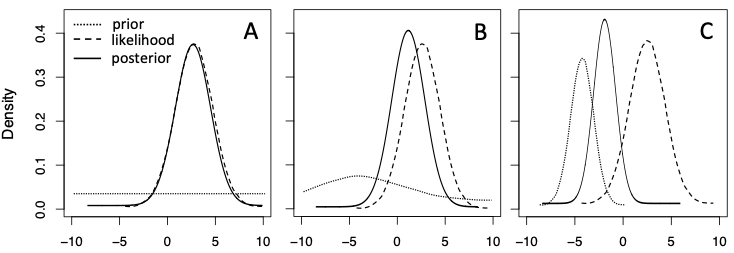
\includegraphics[width=1\linewidth]{parameter_fig} 

}

\caption{\textbf{Prior, likelihood and posterior distribution of a parameter value using; A. noninformative prior; B weakly informative prior; C informative prior.}}\label{fig:param-plot}
\end{figure}

For a model with more than a single parameter, the posterior distribution encapsulates the contribution of all model elements. In this case the posterior distribution is termed the \emph{joint posterior distribution}. If we wish to look at each model parameter separately, we can do this by obtaining the \emph{marginal posterior distribution} for the parameter. We can also examine the posterior distribution for a single parameter with a specific value assigned to the other model parameters; this is called the \emph{conditional posterior distribution}.

Summary statistics can be obtained from the posterior distribution for model coefficients. These are typically the \emph{posterior mean} and \emph{95\% credible intervals}, which are equivalent to maximum likelihood estimates and 95\% confidence intervals in a frequentist GLM. However, unlike confidence intervals, which assume large sample approximations and represent the range of values that contain the true parameter for 95\% of repeated samples, Bayesian credible intervals provide an interval containing the true parameter value with 95\% probability and are appropriate for small samples.

\hypertarget{comp-methods}{%
\section{Bayesian computational methods}\label{comp-methods}}

While Bayesian inference offers a coherent and intellectually satisfying approach to modelling ecological data, computation of posterior distributions involves multidimensional integration, which is computationally highly demanding. In the case of simple conjugate models, exact computation is possible. However, ecological models are rarely appropriate for this approach and calculating the true posterior distribution numerically is problematic. Two alternative computational approaches are available to obtain estimates of posterior distributions; Markov chain Monte Carlo sampling and numerical approximation.

\hypertarget{mcmc}{%
\subsection{Markov chain Monte Carlo sampling (MCMC)}\label{mcmc}}

One option is to draw a Monte Carlo random sample from the joint posterior distribution. A Markov chain Monte Carlo sample drawn from the posterior will approximate the true posterior when the sample size is large. This approach is analogous to treating the posterior distribution as a large population of data from which samples are repeatedly drawn. Each random draw is correlated with the previous, but given a sufficiently large set of samples, the sample distribution should converge on the true population distribution.

There are numerous R packages which can be used to implement MCMC for specific classes of model. For example, the \texttt{BEST} package is a Bayesian alternative to \emph{t} tests. There are also software packages that permit a wide range of MCMC-based Bayesian models to fitted. Examples are \emph{JAGS} and \emph{STAN}. These run separately from R, but can be called from R using specific R packages, for example \texttt{R2jags} in the case of \emph{JAGS}.

While MCMC offers a powerful method for posterior inference, in practice model convergence can be excessively time consuming. MCMC diagnostics is complicated and, because the outcome of MCMC is random, replicability is not assured.

\hypertarget{inla}{%
\subsection{Numerical approximation}\label{inla}}

An alternative to MCMC for obtaining a posterior distribution is offered by an approach that derives approximate solutions to numerical integration. Laplace approximation uses a normal distribution to approximate the posterior distribution and is able to generate accurate approximations. Notably, numerical approximation is substantially faster than MCMC, making exploration of Bayesian models more practical.

Integrated nested Laplace approximation (INLA) is a particularly user-friendly computational method \citep{Rue_2009}. Instead of estimating a multivariate joint posterior distribution, which is difficult to obtain, INLA focuses on individual posterior marginal distributions of model parameters. The INLA R package offers a full suite of Bayesian tools. We use R-INLA throughout this book for fitting Bayesian GLMs and recommend \citet{Wang_2018} and \citet{G_mez_Rubio_2020} for fuller discussion of the theory of INLA.

\hypertarget{bayes-pros}{%
\section{The advantages of Bayesian inference}\label{bayes-pros}}

Bayesian inference offers an alternative framework to the classical frequentist approach and has a number of advantages:

\begin{enumerate}
\def\labelenumi{\arabic{enumi}.}
\item
  Bayesian inference explicitly permits the inclusion of informative priors, enabling existing knowledge or results from a previous model, study, or from expert opinion to inform the current model.
\item
  Bayesian inference treats the data as fixed (which it is), and model parameters to be random (since they are unknowns). In contrast, frequentist inference considers the unknown parameters to be fixed, and the data to be random.
\item
  Bayesian inference provides answers based on the observed data and not based on the distribution of estimators or test statistics from imaginary samples.
\item
  Bayesian inference includes uncertainty in the probability model, yielding more realistic predictions. Frequentist inference does not include uncertainty of parameter estimates, yielding less realistic predictions.
\item
  Bayesian inference estimates a full probability model. Frequentist inference does not and there is no frequentist probability distribution associated with parameters or hypotheses.
\item
  Bayesian inference utilises observed data only. Frequentist inference uses both observed data and future data that is unobserved and hypothetical.
\item
  Bayesian inference permits more complicated models to be fitted than are possible in a frequentist framework.
\item
  Bayesian inference is unbiased with respect to sample size and can accommodate any sample size no matter how small. Frequentist inference becomes more biased as sample size decreases from infinity, and is markedly biased with small samples.
\end{enumerate}

\hypertarget{bayes-critics}{%
\section{Criticism of Bayesian inference}\label{bayes-critics}}

While the Bayesian approach appears to have several advantages over the frequentist approach. It presents new problems of its own, not least its greater complexity. Arguments presented against Bayesian inference typically revolve around the first two advantages of Bayesian inference listed in Section \ref{bayes-pros}:

\begin{enumerate}
\def\labelenumi{\arabic{enumi}.}
\item
  Incorporating a prior introduces subjectivity into statistical modelling.
\item
  Whether data and hypotheses can hold the same status as random variables; i.e.~it is unreasonable to place a probability distribution on model parameters.
\end{enumerate}

A counter to the first argument is that all statistics are demonstrably subjective. From data collection, choice of variables, choice of likelihood, link function, etc. Indeed the choice of threshold for asserting a result to be `statistically significant' is an entirely subjective judgement, and one that is often abused through the practice of `P-hacking'. A Bayesian approach is at least explicit in acknowledging subjectivity and considers how the degree of subjectivity impinges on the conclusions derived from a model.

To the second argument, a Bayesian would argue that whether a parameter should be rightly considered as fixed is irrelevant, since we are uncertain about its true value. As a result, imposing a probability distribution on a parameter is reasonable, since it reflects our uncertainty about a parameter's true value.

\hypertarget{bayes-concl}{%
\section{Conclusions}\label{bayes-concl}}

Bayesian inference offers an alternative framework to data analysis to the classical frequentist approach and has a number of advantages. One is that prior information can be incorporated into an analysis. Using prior information in a model is intuitively appealing and better reflects the scientific method of building on previous knowledge. A second advantage is in avoiding hypothesis testing and P-values, which do not allow us to draw direct conclusions about model parameters; only about hypothetical data that will never be collected. Finally, there is a large range of advanced statistical methods that can only be performed in a Bayesian setting, and for this reason alone ecologists should gain some understanding of the Bayesian approach.

\hypertarget{data-exploration}{%
\chapter{Data exploration}\label{data-exploration}}

Before attempting to analyse data, whether in a frequentist of Bayesian context, it is vital to perform a data exploration. A data exploration will save time by identifying any potential problems in the data and will help in deciding what type of analysis to conduct and model to fit.

\hypertarget{six-step-data-exploration-protocol}{%
\section{Six-step data exploration protocol}\label{six-step-data-exploration-protocol}}

We adopt the protocol proposed by \citet{Zuur_2009} for conducting data exploration. This protocol comprises 6 steps and is intended to identify:

\begin{enumerate}
\def\labelenumi{\arabic{enumi}.}
\tightlist
\item
  Outliers in response and independent variables
\item
  Normality and homogeneity of the response variable
\item
  An excess of zeros in the response variable
\item
  Multicollinearity among independent variables
\item
  Relationships among response and independent variables
\item
  Independence of the response variable
\end{enumerate}

It is good practice to conduct a data exploration, irrespective of the type of data you have or the test you plan to conduct. Here we will conduct a data exploration on the Wytham Wood blue tit data introduced in Chapter 1 from the study by \citet{O_Neill_2018}.

\emph{\textbf{Import data}}

Data are saved in the tab-delimited file \texttt{cyanistes.txt} and are available from \href{https://www.dropbox.com/s/5q3hdyxcouw6ifa/cyanistes.txt}{Dropbox}. Download this file to the same directory (folder) where you save the \texttt{.proj} for this book. This is then easily imported into a dataframe in R using the command:

\texttt{cyan\ \textless{}-\ read.table(file\ =\ "cyanistes.txt",\ header\ =\ TRUE,\ dec\ =\ ".",\ stringsAsFactors\ =\ TRUE)}

Start by inspecting the dataframe using the \emph{structure} function \texttt{str}:

\texttt{str(cyan)}

\begin{verbatim}
'data.frame':   438 obs. of  7 variables:
 $ id    : Factor w/ 377 levels "B1","B10","B111",..: 1 2 ...
 $ zone  : Factor w/ 9 levels "B","C","CP","E",..: 1 1 ...
 $ year  : int  2002 2001 ...
 $ multi : Factor w/ 2 levels "no","yes": 2 2 ...
 $ height: num  2.7 2 ...
 $ day   : int  8 25 ...
 $ depth : num  0.33 0.25 ...
\end{verbatim}

The dataframe comprises 438 observations of 7 variables. Each row in the dataframe represents a record for a blue tit nest. The variable \texttt{id} is a unique identifier for an artificial nest box in which a nest was found. Note that there are fewer levels of id (377) than observations (438), which indicates there are multiple records (in different years) for different nests in the same nest box. This is a potential problem and we will revisit this point in Section \ref{independence}. The variable \texttt{zone} represents different woodland compartments within Wytham Woods; there are nine levels of this categorical variable. These zones represent a discrete stand of trees in the woodland, where the composition of vegetation varies due to historical woodland management practices. The variable \texttt{year} is the year of data collection (varying from 2001-2003). The variable \texttt{multi} is binomial, comprising 1s and 0s, and indicates whether the female that built the nest bred more than once in that year (0 = no, 1 = yes). \texttt{Height} is a continuous variable and is the vertical height (in m) at which the nest box containing the nest was attached to a tree. \texttt{Day} represents the number of days after the 1st April in a given year that the first egg was laid in the nest. Finally, \texttt{depth} is the depth of the nest, recorded as a fraction of the nest box filled. Nest \texttt{depth}, which represents a measure of nest size, may indicate blue tit body condition or access to resources and is the main variable of interest to the researchers who conducted the study -- termed the \emph{response} or \emph{dependent variable}.

Missing data, which are designated \emph{NA} in the tab-delimited file, can be problematic in data analysis. Therefore, it is necessary to check if there are any missing values in the dataframe.

\texttt{colSums(is.na(cyan))}

\begin{verbatim}
    id   zone   year  multi height    day  depth 
     0      0      0      0      0      0      0 
\end{verbatim}

No missing data are associated with any of the variables in the dataframe.

\hypertarget{outliers}{%
\subsection{Outliers}\label{outliers}}

An outlier is an observation that has a relatively large or small value compared to the majority of observations. Many statistical techniques are sensitive to the presence of outliers in data. Outliers are best identified visually, here we use a boxplot (R code for this plot is available in the script associated with this chapter):



\begin{figure}

{\centering 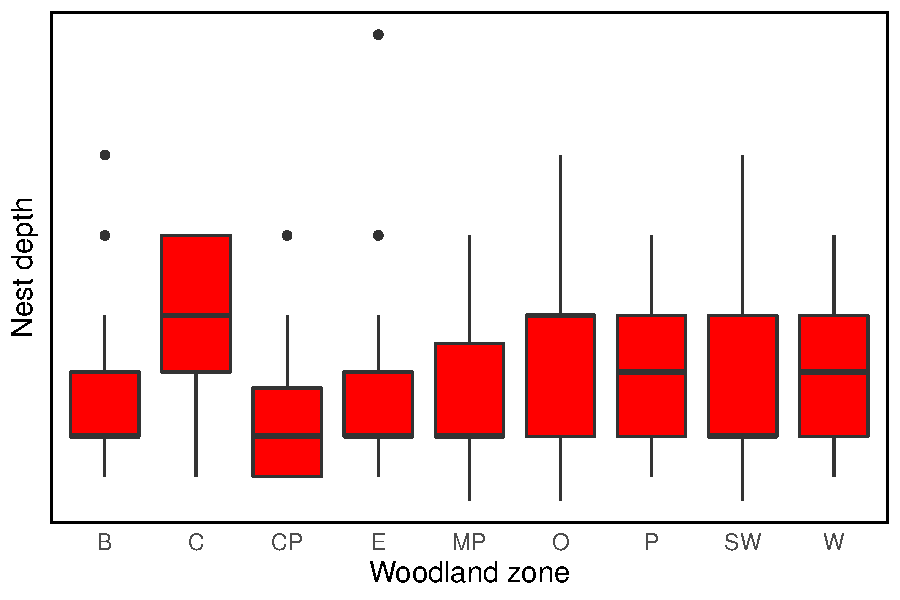
\includegraphics{Bayesian_GLMs_files/figure-latex/ch3-boxplot-cyan-1} 

}

\caption{\textbf{Boxplot of blue tit nest depths for each woodland zone in Wytham Wood.}}\label{fig:ch3-boxplot-cyan}
\end{figure}

Fig. \ref{fig:ch3-boxplot-cyan} visualises the median and spread of the data, with the median represented as a thick horizontal line and the 25\% and 75\% quartiles (the inter quartile range or IQR) represented by the box. The black lines extending from the box represent the range of the data and the black dots are outliers. Outliers are arbitrarily identified as data points that are 3x lower or higher than the IQR. The boxplot shows that there are differences in the average nest depth among woodland zones. This finding suggests that there could be spatial differences in nest size that may be related to vegetation composition, or the birds that occupy different areas of Wytham Woods.

An approach to identify outliers for continuous variables is to use multi-panel Cleveland dotplots, as in Fig. \ref{fig:ch3-cleveland} (R code for this plot is available in the script associated with this chapter):



\begin{figure}

{\centering 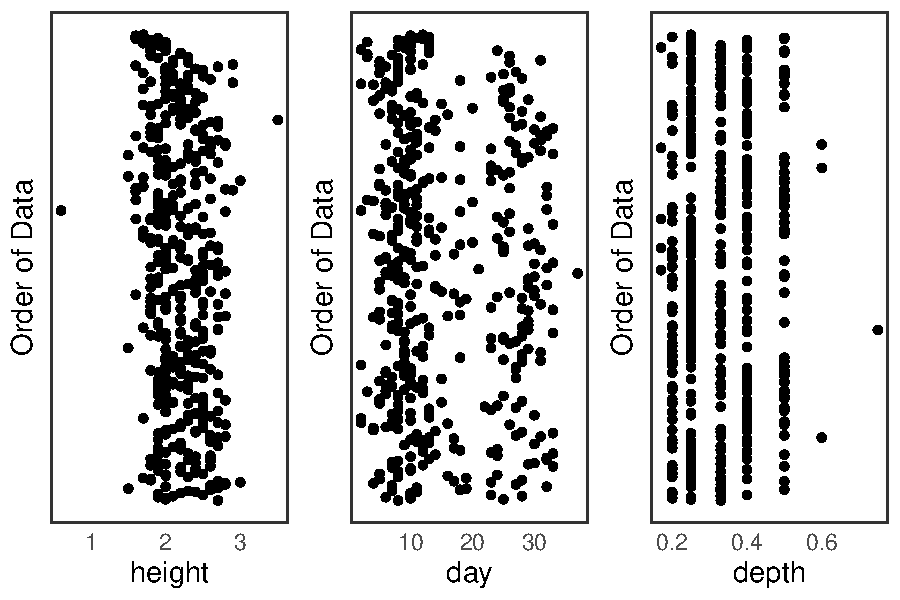
\includegraphics{Bayesian_GLMs_files/figure-latex/ch3-cleveland-1} 

}

\caption{\textbf{Dotplots of the continuous variables height, day and depth. Data are arranged by the order they appear in the dataframe (bottom to top).}}\label{fig:ch3-cleveland}
\end{figure}

The dotplot for \texttt{day} shows no prominent outliers. However, for \texttt{height} there appears to be one nest box that is set unusually low and another unusually high. For \texttt{depth} there is one nest that is unusually deep.

Grubb's test from the \texttt{outliers} package can be used to test whether the value that is farthest (above or below) the mean is an outlier. In this test an outlier is identified from the difference between the outlier value and the mean of all the values, divided by the standard deviation.

For nest depth we will test for a single outlier:

\texttt{outliers::grubbs.test(cyan\$depth,\ type\ =\ 10)}

\begin{verbatim}
    Grubbs test for one outlier

data:  cyan$depth
G = 4.13755, U = 0.96074, p-value = 0.006479
alternative hypothesis: highest value 0.75 is an outlier
\end{verbatim}

Grubb's test shows that the single unusually high depth value (of 0.75) is indeed an outlier (the P-value is lower than the critical threshold of 0.05). However, Grubb's test assumes these data are normally distributed -- something we have yet to test.

For nest box height there is an unusually high and low value. Consequently we modify the test to examine two outliers simultaneously by changing test `type'.

\texttt{outliers::grubbs.test(cyan\$height,\ type\ =\ 11)}

\begin{verbatim}
    Grubbs test for two opposite outliers

data:  cyan$height
G = 8.64561, U = 0.91371, p-value < 2.2e-16
alternative hypothesis: 0.6 and 3.5 are outliers
\end{verbatim}

The test indicates that the low (0.6 m) and high (3.5 m) nest boxes are both outliers. Even where outliers exist, before we consider dropping data from our analysis, we go on with our data exploration, but take note of the variables that have at least one outlier that might influence a subsequent analysis.

On the basis of Fig. \ref{fig:ch3-cleveland} we concluded that there were no outliers in the variable \texttt{day} based on our visual assessment. We can confirm that conclusion with a final Grubb's test.

\texttt{outliers::grubbs.test(cyan\$day,\ type\ =\ 10)}

\begin{verbatim}
    Grubbs test for one outlier

data:  cyan$day
G = 2.41610, U = 0.98661, p-value = 1
alternative hypothesis: highest value 37 is an outlier
\end{verbatim}

The test indicates that the highest value (day 37) is not an outlier since the P-value exceeds 0.05. This means that our visual inspection of the data was accurate. We should not be overly reliant on tests, such as Grubb's test, to make decisions about our data -- visual inspection is often enough.

\hypertarget{normality-and-homogeneity-of-the-dependent-variable}{%
\subsection{Normality and homogeneity of the dependent variable}\label{normality-and-homogeneity-of-the-dependent-variable}}

An assumption of some statistical tests is that the response variable is \emph{normally distributed} at each covariate value. The distribution of a continuous variable can be visualized by dividing the x-axis into `bins' and counting the number of observations in each bin as a frequency polygon using the \texttt{geom\_freqpoly()} function from the \texttt{ggplot2} plotting package:

\texttt{cyan\ \%\textgreater{}\%\ ggplot(aes(depth))\ +\ geom\_freqpoly(bins\ =\ 7)\ +\ labs(x\ =\ "Nest\ depth",\ y\ =\ "Frequency")\ +\ theme\_classic()\ +\ theme(panel.border\ =\ element\_rect(colour\ =\ "black",\ size\ =\ 1))}



\begin{figure}

{\centering 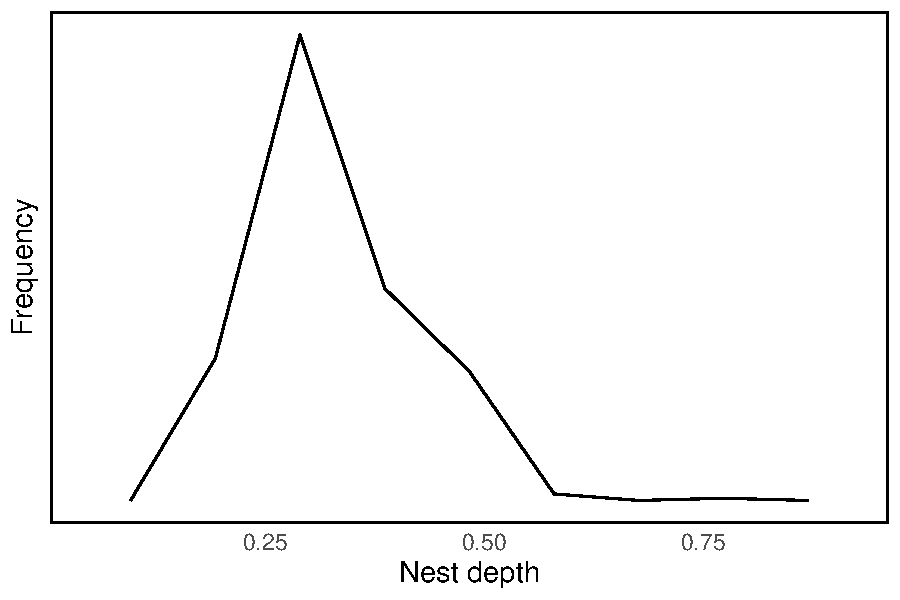
\includegraphics{Bayesian_GLMs_files/figure-latex/ch3-freqpoly-cyan-1} 

}

\caption{\textbf{Frequency polygon of nest depth for blue tits in Wytham Woods.}}\label{fig:ch3-freqpoly-cyan}
\end{figure}

The frequency polygon plot of the dependent variable (Fig. \ref{fig:ch3-freqpoly-cyan}) shows a positive skew, which potentially indicates deviation from normality. However, this figure ignores the factors, such as nest height or zone, that may explain deviation from normality. Given that we already recognise that the distribution of nest depth may vary with woodland zone (Fig. \ref{fig:ch3-boxplot-cyan}), it is not surprising that the data appear as they do. Outliers may also affect the distribution of the dependent variable. At this stage, then, we can proceed with the data exploration bearing in mind that the raw data values for the dependent variable are not perfectly normally distributed.

It is possible to test for normality using the Shapiro-Wilk test. The null hypothesis for this test is that the distribution of the data follows a normal distribution. If the P-value is below 0.05 (P \textless0.05) the null hypothesis is rejected and the conclusion is that the data depart from normality.

\texttt{shapiro.test(cyan\$depth)}

\begin{verbatim}
    Shapiro-Wilk normality test

data:  cyan$depth
W = 0.89872, p-value < 2.2e-16
\end{verbatim}

The test shows significant departure from normality (P \textless0.05).

\emph{Homogeneity of variance} is an even distribution of covariate values around the mean and is another important assumption of many statistical tests. Without homogeneity of variance, estimated P-values are unreliable. There are several ways to measure homogeneity of variance.

To visualise the homogeneity of the response variable in relation to a categorical covariate a boxplot is illustrative. Fig. \ref{fig:ch3-boxplot-cyan} showed variation in the spread of depth data among levels of the factor zone, possibly indicating a lack of homogeneity. A scatterplot is better to visualise homogeneity of variance in relation to a continuous covariate.

\texttt{cyan\ \%\textgreater{}\%\ ggplot(aes(x\ =\ height,\ y\ =\ depth))\ +\ geom\_jitter(\ shape\ =\ 19,\ size\ =\ 2.5,\ height\ =\ 0.05,\ width\ =\ 0.05,\ alpha\ =\ 0.5)\ +\ geom\_hline(yintercept=0.33,\ linetype="dashed")\ +\ geom\_vline(xintercept=2.19,\ linetype="dashed")\ +\ labs(x\ =\ "Nest\ box\ height\ (m)",\ y\ =\ "Nest\ depth")\ +\ xlim(0,4)\ +\ ylim(0,0.8)\ +\ theme\_classic()\ +\ theme(panel.border\ =\ element\_rect(colour\ =\ "black",\ fill=NA,\ size\ =\ 1))}



\begin{figure}

{\centering 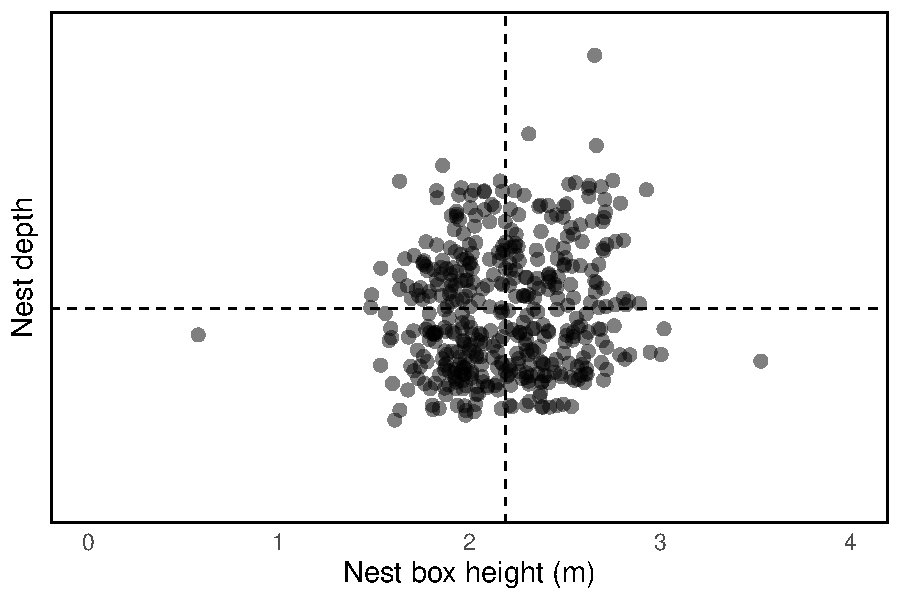
\includegraphics{Bayesian_GLMs_files/figure-latex/ch3-scatter-cyan-1} 

}

\caption{\textbf{Scatterplot of depth and height. The mean for depth and height are added as horizontal and vertical dashed lines, respectively. The distribution of points in the four quadrants are similar, indicating homogeneity of the data.}}\label{fig:ch3-scatter-cyan}
\end{figure}

The scatterplot (Fig. \ref{fig:ch3-scatter-cyan}) shows a symmetrical cloud of points, indicating that the data probably do not deviate significantly from homogeneity.

There are several tests of homogeneity of variance, such as Bartlett's Test, the F-ratio test, and Levene's test. The first two of these assume normality of the data. If your data deviate from normality they should not be used. Levene's test does not assume normality. An alternative is the Brown \& Forsythe test, which uses the median rather than mean in its estimation, and is robust to departures from normality. This test is based on Levene's test and can be obtained using the \texttt{leveneTest()} function from the \texttt{car} package:

\texttt{leveneTest(depth\ \textasciitilde{}\ zone,\ data\ =\ cyan,\ center\ =\ median)}

\begin{verbatim}
Levene's Test for Homogeneity of Variance (center = median)
       Df F value Pr(>F)
group   8  0.6051 0.7738
      429               
\end{verbatim}

Which confirms the data do not deviate from homogeneity (P = 0.774).

\hypertarget{lots-of-zeros-in-the-response-variable}{%
\subsection{Lots of zeros in the response variable}\label{lots-of-zeros-in-the-response-variable}}

Zeros should not be omitted from a dataset. However, an excess of zeros in the response variable, termed `zero inflation', can cause problems with an analysis. Fortunately, there are a number of ways of dealing with zero inflation. The first step is to identify whether there is a potential problem. The percentage of zeros in the response variable can be estimated as:

\texttt{sum(cyan\$depth\ ==\ 0,\ na.rm\ =\ TRUE)\ *\ 100\ /\ nrow(cyan)}

0

There are no zeros in the response variable for this dataset, but it is good practice to always check with your own datasets. If there had been zeros, how many would be too many? The question of how many zeros leads to zero inflation is often asked but cannot be answered without fitting a model and then running simulations from it to see how many zeros are predicted and then compared to the raw data. This procedure is dealt with in Chapters 5 and 6.

\hypertarget{multicollinearity-among-covariates}{%
\subsection{Multicollinearity among covariates}\label{multicollinearity-among-covariates}}

Along with normality of residuals and homogeneity of variance, an additional assumption of analyses that include several predictor variables is independence of the covariates. In ecological studies it is not unusual to collect a large number of environmental or behavioural variables that are often highly correlated. If independent variables in an analysis are correlated the variance associated with predictions will be affected.

Multicollinearity can be tested in several ways. For continuous variables the simplest is to construct a correlation matrix with corresponding pairplots using the \texttt{ggpairs()} function from the \texttt{GGally} package:



\begin{figure}

{\centering 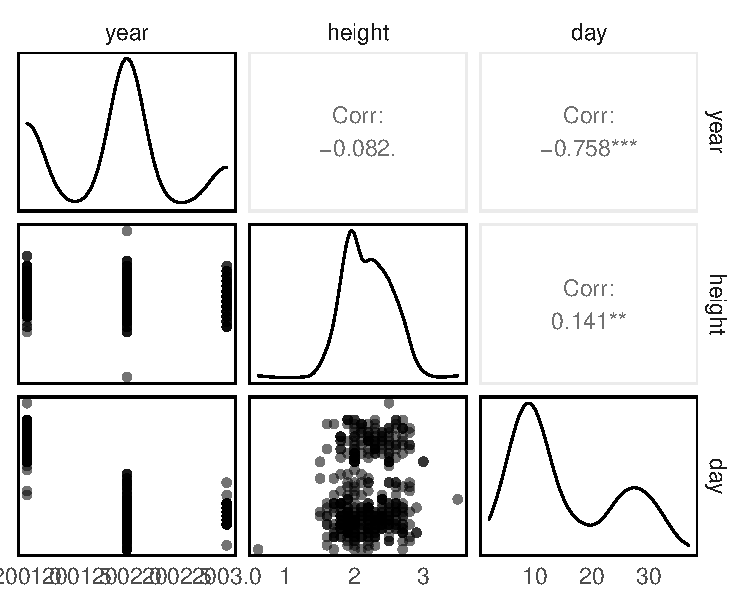
\includegraphics{Bayesian_GLMs_files/figure-latex/ch3-pairs-cyan-1} 

}

\caption{\textbf{Pairplots of year, height and day. Upper right panels show pairwise Pearson correlations, with number of stars proportional to the correlation coefficient (\emph{r}).'}}\label{fig:ch3-pairs-cyan}
\end{figure}

The pairplots (Fig. \ref{fig:ch3-pairs-cyan}) show \texttt{year} and \texttt{day} to be negatively associated ( \emph{r} = -0.76). This is an interesting observation, since it implies that there has been a change in blue tit laying date with year, which may have ecological significance. We need to be aware of this pattern if we plan to use both these variables to make predictions of nest depth.

\hypertarget{relationships-among-dependent-and-independent-variables}{%
\subsection{Relationships among dependent and independent variables}\label{relationships-among-dependent-and-independent-variables}}

Visual inspection of the data using plots is a valuable step and will illustrate what relationships there are between variables in your dataframe. Do not be shy about spending time plotting and summarising your data before formally analysing them -- this is time well spent and will help inform you about the peculiarities of your data and the appropriate way to analyse them.

Below is R script to conduct a multi-panel scatterplot:

\texttt{cyan\ \%\textgreater{}\%\ ggplot(aes(x\ =\ height,\ y\ =\ depth))\ +\ geom\_point()\ +\ geom\_smooth(method\ =\ \textquotesingle{}lm\textquotesingle{},\ colour\ =\ \textquotesingle{}red\textquotesingle{},\ se\ =\ FALSE)\ +\ theme(panel.background\ =\ element\_blank())\ +\ theme(panel.\ border\ =\ element\_rect(fill\ =\ NA,\ size\ =\ 1))\ +\ theme(strip.\ background\ =\ element\_rect(fill\ =\ "white",\ color\ =\ "white",\ size\ =\ 1))\ +\ facet\_wrap(\textasciitilde{}zone)}



\begin{figure}

{\centering 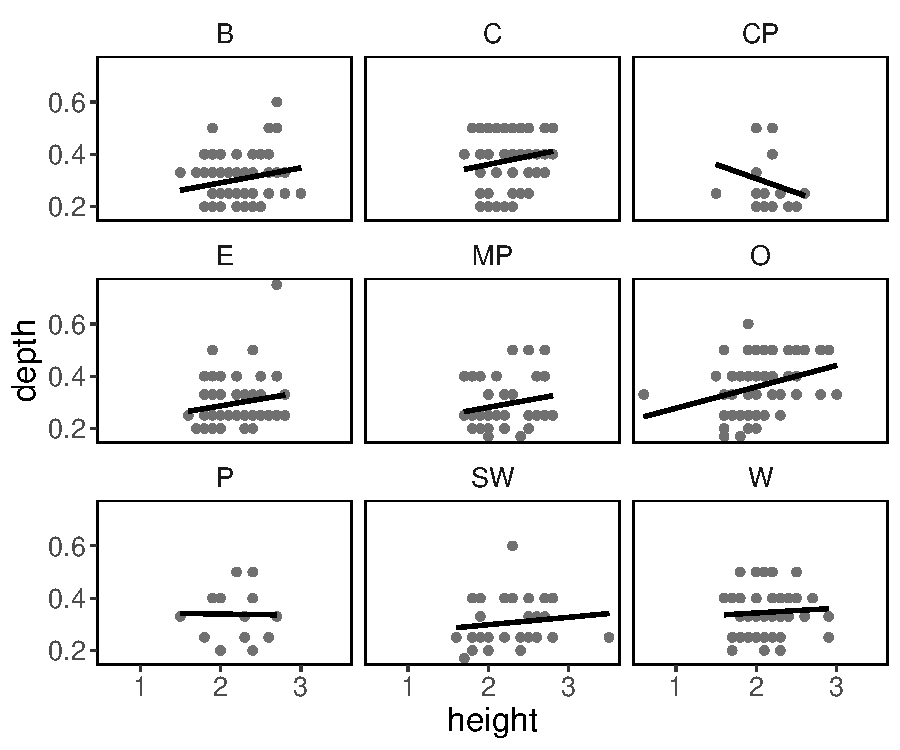
\includegraphics{Bayesian_GLMs_files/figure-latex/ch3-multipanel-cyan-1} 

}

\caption{\textbf{Multipanel scatterplot of blue tit nest depth and nest box height across woodland zones with a line of best fit plotted.}}\label{fig:ch3-multipanel-cyan}
\end{figure}

The plot of the data in Fig. \ref{fig:ch3-multipanel-cyan} does not suggest strongly non-linear patterns. Fitted lines for the relationship between height and depth indicate that the nature of this relationship is different for some woodland zones (e.g.~`O' and `CP'), suggesting that there may be interesting interactions between variables.

\hypertarget{independence}{%
\subsection{Independence of response variable}\label{independence}}

A critical assumption of any data analysis is that each observation in a dataset is independent of all others. For some data this assumption is difficult to confirm but the risk of non-independence can be reduced by careful sampling. Strictly randomly collected samples will tend to be independent.

Additional information, such as spatial location or time of collection, can be included in a dataset. Spatial and temporal dependency in ecological data are common and require specific modelling approaches.

In the case of the Wytham Woods blue tit data, we noted earlier that there are fewer levels of nest box id than observations, which indicates there are multiple records (in different years) for different nests in the same nest box; i.e.~some nests were built in the same nest boxes in different years. This pattern means that every row of data is not strictly independent. This situation is not fatal to an analysis as long as we recognise that there is `dependency' in the data. For now we have two options; the first is to delete rows with duplicate records for the same nest box; though the question then arises of which to remove. A second option is to accept a low level of dependency and report that fact within the results of a data analysis. A more sophisticated solution is to fit nest box id as a `random' term in a General(ised) Linear Mixed Model (GLMM).

\hypertarget{results-of-data-exploration}{%
\section{Results of data exploration}\label{results-of-data-exploration}}

The data exploration showed:

\begin{enumerate}
\def\labelenumi{\arabic{enumi}.}
\tightlist
\item
  An outlier in the response variable depth. There were additional outliers in the explanatory variable height.
\item
  A non-normally distributed but homogenous response variable.
\item
  No zeros in the response variable.
\item
  Collinearity between the variables day and year.
\item
  A potential interaction between depth and zone.
\item
  Dependency in the data due to repeated sampling of the same nest boxes.
\end{enumerate}

If we wish to go further with analysing these data we will need to address the problem of outliers. We will also need to consider non-normality and collinearity. The potential interaction we identified might inform our decisions about what model to fit. Finally, at the very least we need to be aware of the inherent dependency in our data, which we can deal with by dropping some of our data, or accommodating dependency in our analysis.

\hypertarget{conclusions}{%
\section{Conclusions}\label{conclusions}}

Data exploration is a crucial procedure that will save time by identifying potential problems in the data. It will help identify interesting patterns and will inform decisions on what model to fit.

A six-step data exploration involves recognising:

\begin{enumerate}
\def\labelenumi{\arabic{enumi}.}
\tightlist
\item
  Outliers in response and independent variables
\item
  Normality and homogeneity of the response variable
\item
  An excess of zeros in the response variable
\item
  Multicollinearity among independent variables
\item
  Relationships among response and independent variables
\item
  Independence of the response variable
\end{enumerate}

\hypertarget{gen-model}{%
\chapter{Bayesian GLM}\label{gen-model}}

A General Linear Model predicts a dependent (or response) variable, which is continuous and approximately normally distributed, from one or more independent (or predictor) variables. A normal statistical distribution, also referred to as a Gaussian distribution (after the brilliant German mathematician Carl Friedrich Gauss), assumes the data are drawn from a distribution that is symmetric and can be summarised by the arithmetic mean and standard deviation. Independent variables may also be continuous, categorical, or a combination of continuous and categorical. Categorical variables are commonly referred to as \emph{factors}, which have a series of \emph{levels.} For example, a factor might be sex, which has just two levels (male and female).

A GLM comprises three components: 1. the linear predictor, which is a linear function of the predictor variable; 2. the conditional probability distribution of the response variable, which is the distribution of the response variable across the regression line for the given set of predictor variables; 3. the link function, which connects the linear predictor with the mean of the conditional probability distribution.

Choice of conditional probability distribution (such as Gaussian, binomial, Bernoulli, Poisson, gamma, beta, etc.) is not based on the distribution of the raw response variable, but rather on variable characteristics, such as whether the variable is continuous or discrete, bounded or unbounded. Choice of conditional distribution largely determines which link function is most appropriate (such as identity, log, logit, inverse, etc.), though choice of link function can be refined as part of the model fitting process.

\hypertarget{bitterling}{%
\section{European bitterling territoriality}\label{bitterling}}

In this Chapter we fit a Bayesian General Linear Model with a Gaussian conditional distribution and an identity link function to a set of data on male European bitterling (\emph{Rhodeus amarus}) territorial behaviour. Bitterling are small freshwater fish with an unusual breeding system. During the breeding season, male bitterling are aggressively territorial and guard freshwater mussels. Female bitterling develop a long egg-laying tube (`ovipositor') that they use to place their eggs in the gills of the mussel, which the males then fertilise.

A study was conducted in Lake Dědová near Lanžhot in the Czech Republic to measure the response distance of male bitterling to a rival when they were guarding a mussel. Male response distance was measured by gradually moving a model of a male bitterling towards a territorial male that was guarding a mussel. The response distance was the horizontal distance that it was possible to move the model towards a guarded mussel before the territorial male attacked it. After obtaining an estimate of the response distance, territorial males were captured with a hand net and their length measured, after which they were immediately released.

In addition, males were randomly allocated to a food supplement treatment, with approximately half the males in the study receiving a 1 g cube of freeze-dried \emph{Tubifex} worms daily for six days before the start of data recording. The remaining males received no food supplement, but did experience disturbance each day that was comparable to those receiving a food supplement.

A two-day pilot study with 8 individuals was also conducted. Data from the pilot study were used to assign prior distributions to fixed parameters in the model.

\emph{\textbf{Import data}}

Data for European bitterling are saved in a comma-separated values (CSV) file \texttt{bitterling.csv} and are imported into a dataframe in R using:

\texttt{bitt\ \textless{}-\ read\_csv("bitterling.csv")}

Start by inspecting dataframe \texttt{bitt}:

\texttt{str(bitt)}

\begin{verbatim}
spec_tbl_df [48 x 4] (S3: spec_tbl_df/tbl_df/tbl/data.frame)
 $ male     : num [1:48] 1 2 3 4 5 ...
 $ sl       : num [1:48] 37 58 50 52 42 ...
 $ supp_feed: num [1:48] 0 0 0 1 0 ...
 $ resp_dist: num [1:48] 114 172 168 185 135 ...
 - attr(*, "spec")=
  .. cols(
  ..   male = col_double(),
  ..   sl = col_double(),
  ..   supp_feed = col_double(),
  ..   resp_dist = col_double()
  .. )
\end{verbatim}

The dataframe comprises 48 observations of 4 variables. Each row in the dataframe represents an observation for a different male bitterling (\texttt{male}). The variable \texttt{sl} is continuous and represents the standard length (in mm) of each male bitterling, while the variable \texttt{supp\_feed} is categorical (though coded numerically) indicating those males that received no food supplement (\texttt{0}) and those that did (\texttt{1}). The variable \texttt{resp\_dist} is the aggressive response distance (in cm) and is the response (dependent) variable of interest.

\hypertarget{glm-steps}{%
\section{Steps in fitting a Bayesian GLM}\label{glm-steps}}

We will follow the 9 steps to fitting a Bayesian GLM, detailed in Chapter 2:

\emph{1. State the question}

\emph{2. Perform data exploration}

\emph{3. Select a statistical model}

\emph{4. Specify and justify a prior distribution on parameters}

\emph{5. Fit the model}

\emph{6. Obtain the posterior distribution}

\emph{7. Conduct model checks}

\emph{8. Interpret and present model output}

\emph{9. Visualise the results}

\hypertarget{state-the-question}{%
\subsection{State the question}\label{state-the-question}}

This study was conducted to understand the extent to which the territorial behaviour of male bitterling is a function of male size and body condition. Our predictions were that larger males would be more effective in responding to intruders to their territory than smaller males. A further prediction was that, given that territoriality is energetically expensive, and males are often constrained in their feeding while engaged in territory defence, supplementing the diets of males would also increase the aggressive response distance of males. A final prediction was that these two variables would interact; specifically that the effect of body size on response distance would be less pronounced in males that received a food supplement; i.e.~energy depletion is more severe for larger males.

Consequently there are three specific predictions to test:

\begin{enumerate}
\def\labelenumi{\arabic{enumi}.}
\item
  A positive association between male body size, measured as standard length (\texttt{sl}), and response distance (\texttt{resp\_dist}).
\item
  A positive association between provision of supplementary food (\texttt{supp\_feed}) and response distance.
\item
  An interaction between male body size and supplementary feeding and response distance, with a steeper slope between body size and response distance for males that did not receive supplementary food.
\end{enumerate}

\hypertarget{data-exploration-1}{%
\subsection{Data exploration}\label{data-exploration-1}}

As with any analysis, whether Bayesian or frequentist, we start by conducting a data exploration to identify any potential problems with the data. First check for missing data.

\texttt{colSums(is.na(bitt)}

\begin{verbatim}
     male        sl supp_feed resp_dist 
        0         0         0         0 
\end{verbatim}

No missing data.

\hypertarget{outliers-1}{%
\subsubsection{Outliers}\label{outliers-1}}

Outliers in the data can identified visually using multi-panel Cleveland dotplots (R code is available in the R script associated with this chapter):



\begin{figure}

{\centering 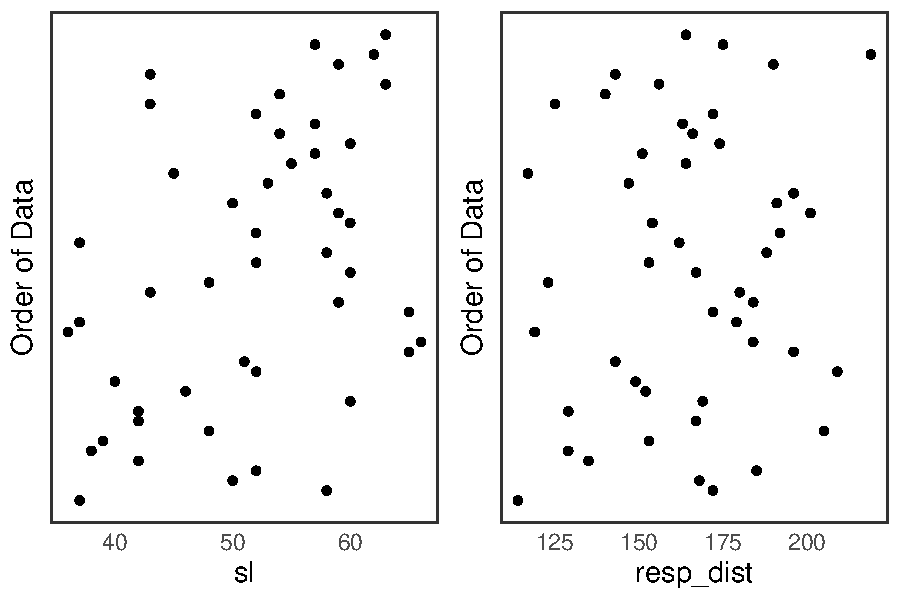
\includegraphics{Bayesian_GLMs_files/figure-latex/ch4-dotplot-1} 

}

\caption{\textbf{Dotplots of male standard length (mm) and aggressive response distance (cm) of European bitterling. Data are arranged by the order they appear in the dataframe.}}\label{fig:ch4-dotplot}
\end{figure}

There are no outliers in Fig. \ref{fig:ch4-dotplot}.

\hypertarget{normality-and-homogeneity-of-the-dependent-variable-1}{%
\subsubsection{Normality and homogeneity of the dependent variable}\label{normality-and-homogeneity-of-the-dependent-variable-1}}

An assumption of a Bayesian Gaussian GLM is that the response variable is normally distributed at each level of the covariate values. The distribution of a continuous variable can be visualized by dividing the x-axis into ``bins'' and counting the number of observations in each bin as a frequency polygon using the \texttt{geom\_freqpoly()} function from the \texttt{ggplot2} package:

\texttt{bitt\ \%\textgreater{}\%\textquotesingle{}}
\texttt{ggplot(aes(resp\_dist))\ +}
\texttt{geom\_freqpoly(\ bins\ =\ 6)\ +}
\texttt{labs(x\ =\ "Response\ distance\ (cm)",\ y\ =\ "Frequency")\ +}
\texttt{My\_theme}



\begin{figure}

{\centering 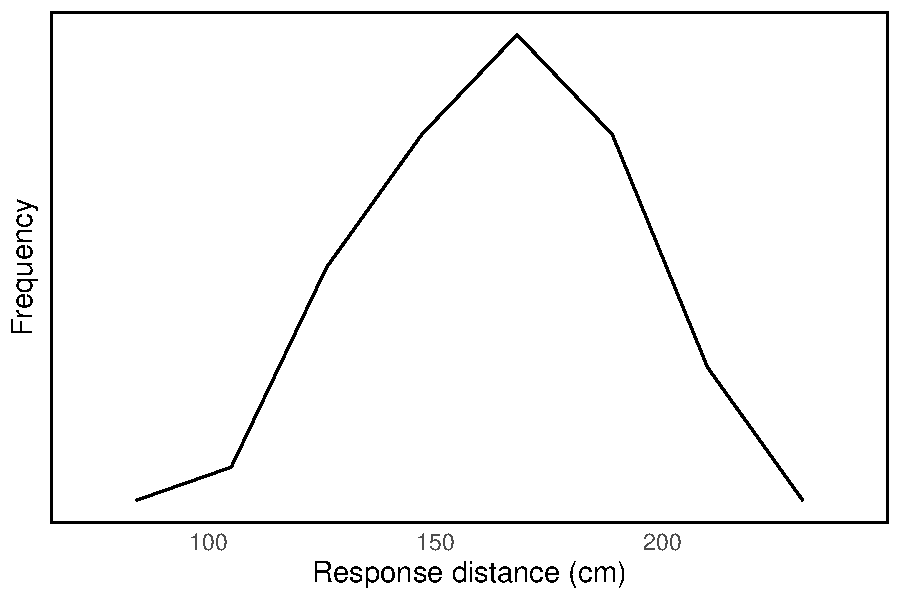
\includegraphics{Bayesian_GLMs_files/figure-latex/ch4-freqpoly-1} 

}

\caption{\textbf{Frequency polygon of response distance (cm) of male European bitterling to the model of a rival.}}\label{fig:ch4-freqpoly}
\end{figure}

The frequency polygon plot of the dependent variable (Fig. \ref{fig:ch4-freqpoly}) shows a distribution that looks approximately normal.

\hypertarget{balance-of-categorical-variables}{%
\subsubsection{Balance of categorical variables}\label{balance-of-categorical-variables}}

The categorical variable for the supplementary feeding treatment (\texttt{supp\_feed}) is coded numerically (0 = no supplementary feeding, 1 = supplementary feeding). This variable needs to be designated as a factor.

\texttt{bitt\$Supp\ \textless{}-\ factor(bitt\$supp\_feed)}

We then examine the balance of this variable:

\texttt{table(bitt\$fSupp)}

\begin{verbatim}
 0  1 
25 23 
\end{verbatim}

Balance is not perfect, with 25 males in the no supplementary feeding treatment and 23 receiving supplementary feeding, but the balance is acceptable.

\hypertarget{multicollinearity-among-covariates-1}{%
\subsubsection{Multicollinearity among covariates}\label{multicollinearity-among-covariates-1}}

Along with normality of residuals and homogeneity of variance, an additional assumption of linear modelling is independence of the independent variables. In ecological studies it is not unusual to collect a large number of variables, which are often highly correlated. If covariates in a model are correlated, then the model may produce unstable parameter estimates with inflated standard errors.

Multicollinearity can be tested in several ways. We can obtain a comprehensive summary of the relationship between the two model covariates using the \texttt{ggpairs} command from the \texttt{GGally} package:

\texttt{bitt\ \%\textgreater{}\%\ ggpairs(columns\ =\ c("sl",\ "fSupp"),\ aes(colour\ =\ fSupp,\ alpha\ =\ 0.8),\ lower\ =\ list(continuous\ =\ "smooth\_loess",\ combo\ =\ wrap("facethist",\ binwidth\ =\ 5)))\ +\ My\_theme}



\begin{figure}

{\centering 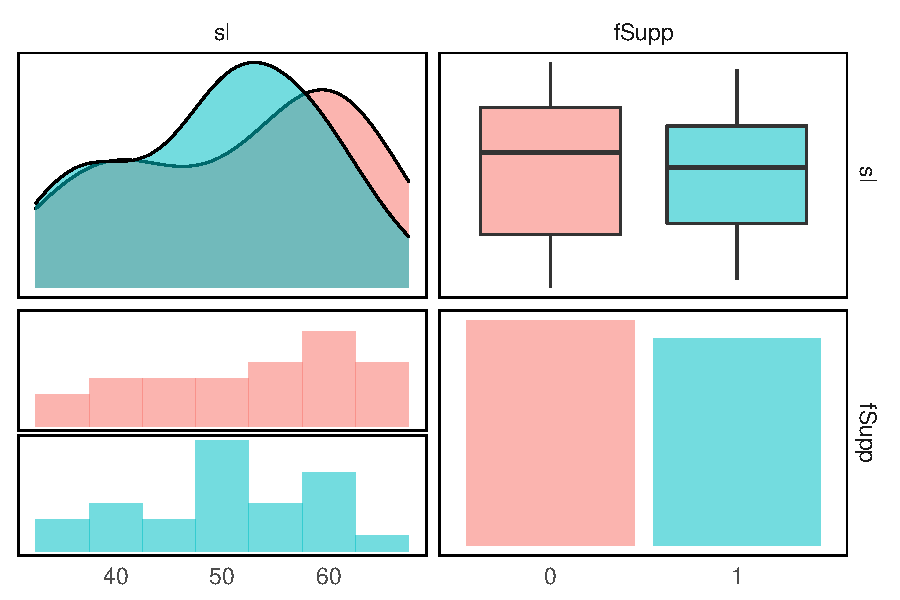
\includegraphics{Bayesian_GLMs_files/figure-latex/ch4-ggpairs-1} 

}

\caption{\textbf{Plot matrix of bitterling standard length (mm) and supplementary feeding treatment. The top left panel shows a frequency plot of standard length split by feeding treatment, while the top right shows the same data expressed as a boxplot. The lower left panel shows a length-frequency histogram of standard lengths, with those for males that did not receive supplementary feeding above and those that did, below. The lower right panel shows the total number of individual males in each supplementary feeding treatment.}}\label{fig:ch4-ggpairs}
\end{figure}

The plot matrix in Fig. \ref{fig:ch4-ggpairs} demonstrates no clear pattern of collinearity between the two covariates and illustrates good overlap in male standard length between levels of the (randomly assigned) feeding treatment.

Another approach to identifying multicollinearity is by calculating a variance inflation factor (VIF) for each variable. The VIF is an estimate of the proportion of variance in one predictor explained by all the other predictors in the model. A VIF of 1 indicates no collinearity. VIF values above 1 indicate increasing degrees of collinearity. VIF values exceeding 3 are considered problematic \citep{Zuur_2009}, in which case the variable with the highest VIF should be removed from the model and the VIFs for the model recalculated.

The VIF for a model can be estimated using the \texttt{vif} function from the \texttt{car} package:

\texttt{round(vif(lm(resp\_dist\ \textasciitilde{}\ sl\ +\ fSupp,\ data\ =\ bitt)),2)}

1.01, 1.01

For the bitterling model the estimated VIFs are \textless3, so there is no problem with multicollinearity.

\hypertarget{zeros-in-the-response-variable}{%
\subsubsection{Zeros in the response variable}\label{zeros-in-the-response-variable}}

Zeros should not be omitted from a dataset. However, an excess of zeros in the response variable, termed `zero inflation', can cause problems with an analysis. The number of zeros in the response variable can be calculated with:

\texttt{sum(bitt\$\ resp\_dist\ ==\ 0)}

\begin{verbatim}
[1] 0
\end{verbatim}

There are no zeros in the response variable, indicating that all territorial males responded aggressively to intruders.

\hypertarget{relationships-among-dependent-and-independent-variables-1}{%
\subsubsection{Relationships among dependent and independent variables}\label{relationships-among-dependent-and-independent-variables-1}}

Visual inspection of the data using plots is a critical step and will illustrate whether relationships are linear or non-linear and whether there are interactions between covariates. R code for this plot is available in the R script associated with this chapter.



\begin{figure}

{\centering 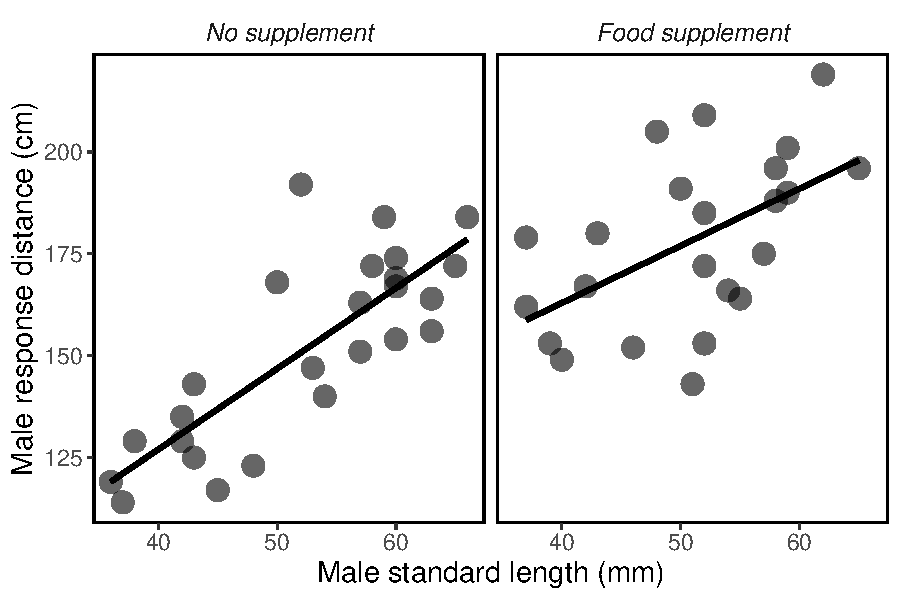
\includegraphics{Bayesian_GLMs_files/figure-latex/ch4-rels-bitt-1} 

}

\caption{\textbf{Multipanel scatterplot of male response distance (cm) and standard length (mm) of European bitterling either without or receiving supplementary feeding with a line of best fit plotted.}}\label{fig:ch4-rels-bitt}
\end{figure}

The plot of the data in Fig. \ref{fig:ch4-rels-bitt} does not indicate a non-linear pattern in the data. However, fitted lines for the relationship between male response distance (cm) and standard length (mm) do suggest that the nature of this relationship may vary with feeding treatment, implying a potential interaction between fish size and feeding treatment; i.e.~the slopes differ between treatments. An interaction would mean that the relationship between response distance and standard length depends on nutritional state. Interactions like this one are biologically interesting. Given the pattern in these data, inclusion of an interaction term in the model is justified.

\hypertarget{independence-of-response-variable}{%
\subsubsection{Independence of response variable}\label{independence-of-response-variable}}

An assumption for a GLM is that each observation in a dataset is independent of all others. In the case of the present study each row of data was a different male bitterling. The study was conducted over a short period (10 days) at the peak of the spawning season of the species in a single lake, which reduced the risk of any strong temporal and spatial effects. Observations were also made by a single experimenter, limiting the risk of dependency in the data due to variation in observer bias. On this basis, we will assume the data are independent.

\hypertarget{selection-of-a-statistical-model}{%
\subsection{Selection of a statistical model}\label{selection-of-a-statistical-model}}

The study was designed specifically to understand the extent to which the territorial behaviour of male European bitterling is a function of male size and nutritional state. The dependent variable is male response distance, which the data exploration showed to be continuous and approximately normally distributed (Fig. \ref{fig:ch4-freqpoly}). There are no zeros in the response variable and there is good reason to believe data are independent. The relationship between male standard length and response distance is approximately linear, irrespective of food supplementation (Fig. \ref{fig:ch4-rels-bitt}).

Given these findings, a Gaussian is an appropriate distribution as a starting point, in combination with an \emph{identity} link function (essentially no link function). Two covariates will be included in the model; male standard length (continuous) and food supplementation (categorical, with two levels) as well as their interaction, which means the model will have five parameters; an intercept (\(\beta_1\)), a slope for standard length (\(\beta_2\)), food supplementation (\(\beta_3\)), and the interaction between standard length and food supplementation (\(\beta_4\)), and the variance (\(\sigma^2\)) of the normal distribution for male response distance.

In the context of an INLA model, the variance parameter is termed a \emph{hyperparameter}. In a simple linear model the hyperparameter just comprises the model residual variance. However, in more complex models the hyperparameter may also include other variance components, such as the random effects in a mixed model or the smoother in a Generalised Additive Model (GAM).

For computational efficiency, Bayesian analysis uses the precision (\(\tau\) or tau) of parameters rather than variance. Precision is the reciprocal of the variance (\(\sigma^{2}\)), thus:

\(\tau\) = \(\sigma^{-2}\)

By default a diffuse gamma prior is assumed for the precision in INLA.

\hypertarget{specification-of-priors}{%
\subsection{Specification of priors}\label{specification-of-priors}}

A key aspect of any Bayesian model are the priors placed on model parameters. While there has been a tendency by ecologists to use non-informative or weakly informative priors, carefully formulated informative priors offer a powerful approach to modelling data, taking the modelling process beyond a description of the data and incorporating additional data or previous findings in a model (see Chapter 2).

\hypertarget{pilot}{%
\subsubsection{Pilot study}\label{pilot}}

In the study described here, a 2-day pilot experiment was conducted before the main study. This pilot study provided an opportunity for refining data collection methods and to obtain model priors. A total of 8 males were tested in the pilot experiment, with 4 receiving a food supplement and 4 with no supplement. In the pilot study several alternative food supplements were used, which meant the protocol followed was not identical to the main study, though the findings broadly matched the observations from the main study.

\emph{\textbf{Import pilot data}}

Pilot data are saved in the tab-delimited file pilot.txt and are imported into a dataframe in R using the command:

\texttt{pilot\ \textless{}-\ read\_tsv("pilot.txt")}

Note we use the \texttt{read\_tsv()} function from the \texttt{readr} package which is part of the \texttt{tidyverse} set of packages.

Start by inspecting the dataframe:

\texttt{str(pilot)}

\begin{verbatim}
spec_tbl_df [8 x 4] (S3: spec_tbl_df/tbl_df/tbl/data.frame)
 $ order     : num [1:8] 1 2 3 4 5 6 7 8
 $ supplement: chr [1:8] "no" "no" "yes" "no" ...
 $ length    : num [1:8] 63 54 64 45 39 60 43 49
 $ distance  : num [1:8] 86 85 160 74 95 118 95 112
 - attr(*, "spec")=
  .. cols(
  ..   order = col_double(),
  ..   supplement = col_character(),
  ..   length = col_double(),
  ..   distance = col_double()
  .. )
\end{verbatim}

The dataframe comprises 8 observations of 4 variables. Each row in the dataframe represents a record for an individual male bitterling. The variables are the numerical variable \texttt{order} which represents the order in which the males were tested, the categorical variable \texttt{supplement} with two levels; \texttt{no} and \texttt{yes}, indicating which individuals received a food supplement. The two other variables in the dataframe are \texttt{length} and \texttt{distance}, corresponding with individual male standard length (mm) and male response distance to an intruder (cm). These are both numerical continuous variables.

\hypertarget{frequentist-linear-model}{%
\subsubsection{Frequentist linear model}\label{frequentist-linear-model}}

We will proceed by fitting a simple (frequentist) general linear model (GLM) to obtain parameter estimates to use as priors. The model is fitted as:

\texttt{p1\ \textless{}-\ lm(distance\ \textasciitilde{}\ length\ +\ supplement,\ data\ =\ pilot)}

A neat numerical output is obtained with the \texttt{tidy} function from the \texttt{broom} package:

\texttt{broom::tidy(p1)}

\begin{verbatim}
# A tibble: 3 x 5
  term          estimate std.error statistic p.value
  <chr>            <dbl>     <dbl>     <dbl>   <dbl>
1 (Intercept)      19.9     36.1       0.552  0.605 
2 length            1.27     0.684     1.86   0.123 
3 supplementyes    34.0     12.2       2.78   0.0390
\end{verbatim}

\begin{enumerate}
\def\labelenumi{\arabic{enumi}.}
\tightlist
\item
  The response distance of males when standard length is zero is approximately 20 cm (sd \textasciitilde{} 40). This is the \texttt{intercept}.
\item
  A 1 mm increase in male standard length results in an increased response distance of approximately 1.3 cm (sd \textasciitilde{} 0.7). This is the slope of \texttt{length}.
\item
  Supplementary feeding adjusted the slope (response distance) by approximately 35 cm (sd \textasciitilde{} 15) (\texttt{supplementyes}).
\end{enumerate}

Since we did not include an interaction in the pilot model it will be incorporated as a weakly-informative prior in the full Bayesian model.

\hypertarget{priors-on-the-fixed-effects}{%
\subsubsection{Priors on the fixed effects}\label{priors-on-the-fixed-effects}}

These findings can be specified in the model as priors on the fixed effects as:

\(\beta intercept\) \textasciitilde{} \emph{N}(20, 1600) (mean, variance)

\(\beta sl\) \textasciitilde{} \emph{N}(1.3, 0.49)

\(\beta fSupp\) \textasciitilde{} \emph{N}(35, 225)

\(\beta interaction\) \textasciitilde{} \emph{N}(0, 1000)

Thus, in the case of \(\beta intercept\), we assume normality with a mean of 20 cm and variance of 1600 (sd = 40) cm.

\hypertarget{priors-on-the-hyperparameter}{%
\subsubsection{Priors on the hyperparameter}\label{priors-on-the-hyperparameter}}

The prior distribution on the hyperparameter should also be specified. The default is a diffuse gamma distribution, but other distributions can be used, for a full list of available distributions in INLA see:

\texttt{names(inla.models()\$prior)}

In addition to these available prior distributions, it is also possible to define your own. In this model we will use a Gaussian distribution with a weakly-informative prior.

\(\sigma\) \textasciitilde{} \emph{N}(0, 1)

Model variance is assumed to be normal, with a mean of 0 and variance of 1.

\hypertarget{fit-the-model}{%
\subsection{Fit the model}\label{fit-the-model}}

We will fit two Bayesian Gaussian GLMs using INLA, one with default priors (\texttt{M0}) and the second with informative priors on the fixed effects, derived from the pilot study, and weakly informative priors on the hyperparameter (\texttt{M1}).

The default INLA model is fitted with the following script:

\texttt{M0\ \textless{}-\ inla(resp\_dist\ \textasciitilde{}\ sl\ *\ fSupp,\ data\ =\ bitt)}

The default priors used for the model can be obtained with:

\texttt{inla.priors.used(M0)}

This output shows that for the fixed effects the priors for the default model are:

\(\beta intercept\) \textasciitilde{} \emph{N}(0, 0) (\(\tau\) = 0)

\(\beta sl\) \textasciitilde{} \emph{N}(0, 1000) (\(\tau\) = 0.001)

\(\beta fSupp\) \textasciitilde{} \emph{N}(0, 1000) (\(\tau\) = 0.001)

\(\beta interaction\) \textasciitilde{} \emph{N}(0, 1000) (\(\tau\) = 0.001)

And for the hyperparameter:

\(\sigma\) \textasciitilde{} loggamma (1, 2 x \(10^{5}\)) (\(\tau\) = 1 x \(5^{-6}\))

The model with informative priors is fitted with the following script:

\texttt{M1\ \textless{}-\ inla(resp\_dist\ \textasciitilde{}\ sl\ *\ fSupp,\ data\ =\ bitt,\ control.family\ =\ list(hyper\ =\ list(prec\ =\ list(prior\ =\ "gaussian",\ param\ =\ c(0,\ 1)))),\ control.fixed\ =\ list(mean.intercept\ =\ 20,\ prec.intercept\ =\ 40\^{}(-2),\ mean\ =\ list(sl\ =\ 1.3,\ fSupp1\ =\ 35,\ default\ =\ 0),\ prec\ =\ list(sl\ =\ 0.7\^{}(-2),\ fSupp1\ =\ 15\^{}(-2),\ default\ =\ 31.62\^{}(-2))))}

The priors can be obtained with:

\texttt{inla.priors.used(M1)}

This output shows that for the fixed effects:

\(\beta intercept\) \textasciitilde{} \emph{N}(20, 1600) (\(\tau\) = 6.25 x \(10^{-5}\))

\(\beta sl\) \textasciitilde{} \emph{N}(1.3, 0.49) (\(\tau\) = 2.04)

\(\beta fSupp\) \textasciitilde{} \emph{N}(35, 225) (\(\tau\) = 4.44 x \(10^{-3}\))

\(\beta interaction\) \textasciitilde{} \emph{N}(0, 1000) (\(\tau\) = 0.001)

And for the hyperparameter:

\(\sigma\) \textasciitilde{} \emph{N}(0, 1) (\(\tau\) = 1)

\hypertarget{obtain-the-posterior-distribution}{%
\subsection{Obtain the posterior distribution}\label{obtain-the-posterior-distribution}}

\hypertarget{model-with-default-priors}{%
\subsubsection{Model with default priors}\label{model-with-default-priors}}

\hypertarget{fixed-effects}{%
\paragraph{Fixed effects}\label{fixed-effects}}

Output from model \texttt{M0} can be obtained with:

\texttt{summary(M0)}

However, this command produces an intimidating cascade of information (not shown here).

An alternative is to look first at the posterior mean, standard deviation and 95\% credible intervals for the fixed effects:

\texttt{M0Betas\ \textless{}-\ M0\$summary.fixed{[},c("mean",\ "sd",\ "0.025quant",\ "0.975quant"){]}}

\texttt{round(M0Betas,\ digits\ =\ 2)}

\begin{verbatim}
             mean    sd 0.025quant 0.975quant
(Intercept) 59.07 17.01      25.91      92.88
sl           1.77  0.32       1.13       2.40
fSupp1      32.35 21.50     -10.41      74.11
sl:fSupp1   -0.07  0.42      -0.88       0.75
\end{verbatim}

This output reports the \emph{posterior mean} and \emph{standard deviation} for the model intercept (\texttt{intercept}), covariates (\texttt{sl}, \texttt{fSupp1}) and interaction (\texttt{sl:fSupp1}). Note that there are no P-values, which are used in frequentist analyses but are meaningless in a Bayesian context. Instead we have the 95\% \emph{credible intervals}; these are the 0.025 and 0.975 quantiles in the output above.

For the variable \texttt{sl} we have a posterior mean of 1.77 and lower 95\% credible interval of 1.13 and upper 95\% credible interval of 2.4. We can conclude from this result that we are 95\% certain that the posterior mean of the regression parameter for \texttt{sl} falls between these credible intervals.

Because the credible intervals for \texttt{sl} do not encompass zero, we can be confident that the slope of the relationship is greater than zero. That is, we are 95\% certain that the true value of the \texttt{sl} parameter in our model is between 1.13 and 2.4 given the data and (default) prior information provided to the model. In a Bayesian context we cannot consider this result `significant', because significance testing only applies in a frequentist hypothesis testing setting. However, we can conclude that \texttt{sl} is \emph{statistically important} in the default model.

Similarly, we can conclude that the \texttt{Intercept} of the relationship, with credible intervals from 25.91 to 92.88, differs from zero with a posterior mean of 59.07 and standard deviation of 17.01.

For supplementary feeding (\texttt{fSupp1}), and the interaction between standard length and supplementary feeding (\texttt{sl:fSupp1}), the credible intervals range from negative values for the lower credible interval to positive for the upper interval, indicating that these model parameters do not differ from zero.

Instead of just summarising the posterior distribution of the fixed effects with a posterior mean and a 95\% credible interval, we can plot the posterior distribution of each parameter, available in the INLA object \texttt{M0\$marginals.fixed}.
The posterior distributions can be visualized using \texttt{ggplot2}. The coding for this plot is available in the R script associated with this chapter.



\begin{figure}

{\centering 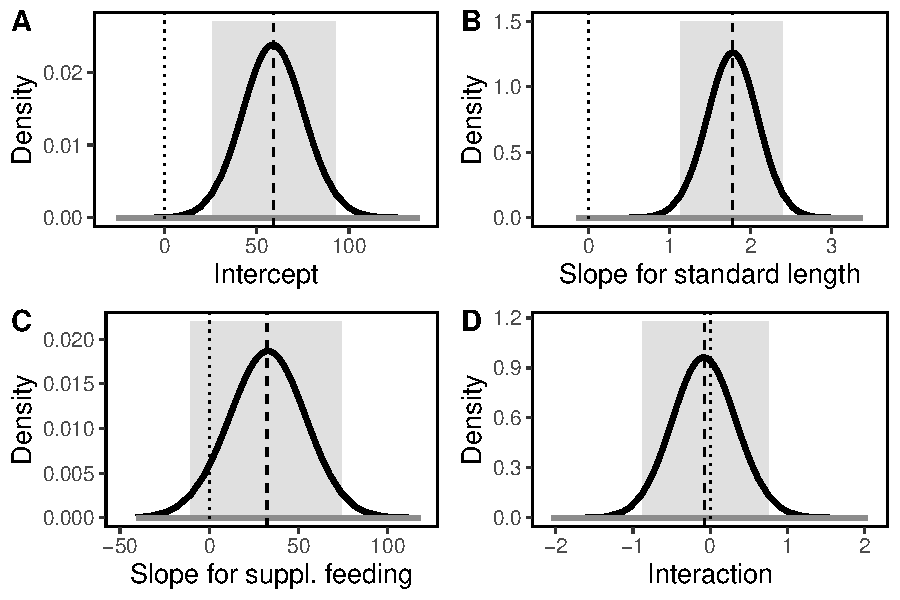
\includegraphics{Bayesian_GLMs_files/figure-latex/ch4-M0-betas-1} 

}

\caption{\textbf{Posterior and prior distributions for fixed parameters of a Bayesian linear regression to predict the territorial response distance of male European bitterling in response to a rival. The model is fitted with default (non-informative) priors. Distributions for: A. model intercept; B. slope for male standard length; C. slope for supplementary feeding; D. interaction of male standard length and supplementary feeding. The solid black line is the posterior distribution, the solid gray line is the prior distribution, the gray shaded area encompasses the 95\% credible intervals, the vertical dashed line is the posterior mean of the parameter, the vertical dotted line indicates zero.}}\label{fig:ch4-M0-betas}
\end{figure}

Figure \ref{fig:ch4-M0-betas} provides a visual representation of the summary of the fixed effects. For parameters where zero (indicated by the dotted line) falls outside the range of the 95\% credible intervals (gray shaded area), the parameter is considered statistically important. Thus, the intercept (panel A) and slope for male standard length (panel B) differ from zero and are statistically important, while the slope for supplementary feeding and interaction between standard length and supplementary feeding are not (i.e.~panels C and D). This figure also shows the non-informative priors, which appear flat across the range of possible values (hence non-informative priors are sometimes termed `flat' priors), and make a limited contribution to the posterior distribution.

\hypertarget{hyperparameter}{%
\paragraph{Hyperparameter}\label{hyperparameter}}

Model \texttt{M0} contains a parameter, sigma (\(\sigma\)), that is used for the variance (\(\sigma{^2}\)) of the normal distribution for male response distance. In the context of an INLA model, the variance parameter is termed a `hyperparameter'. In a simple linear model like \texttt{M0} the hyperparameter just comprises the model residual variance.

As with the fixed effects, we can put priors on the hyperparameter (or use the non-informative default) but a vital step in fitting a Bayesian model is to examine the posterior distribution of the hyperparameter(s).

Recall that a slight complication is that INLA uses precision (\(\tau\) or tau) rather than the variance of the hyperparameter, though this is simply the reciprocal of the variance.

We can obtain a summary of the precision of the hyperparameter with:

\texttt{M0hyp\ \textless{}-\ M0\$summary.hyper{[},c("mean",\ "mode",\ "0.025quant",\ "0.975quant"){]}}

\begin{longtable}[]{@{}ccccc@{}}
\toprule
& mean & mode & 0.025quant & 0.975quant \\
\midrule
\endhead
Precision for Gaussian obs & 0.004 & 0.0038 & 0.0025 & 0.0057 \\
\bottomrule
\end{longtable}

The posterior distribution of the precision of the hyperparameter can be visualized using \texttt{ggplot2}. See the R script associated with this chapter. Because the posterior distribution is not symmetrical, we plot the posterior mode (rather than mean) as a dashed vertical line.



\begin{figure}

{\centering 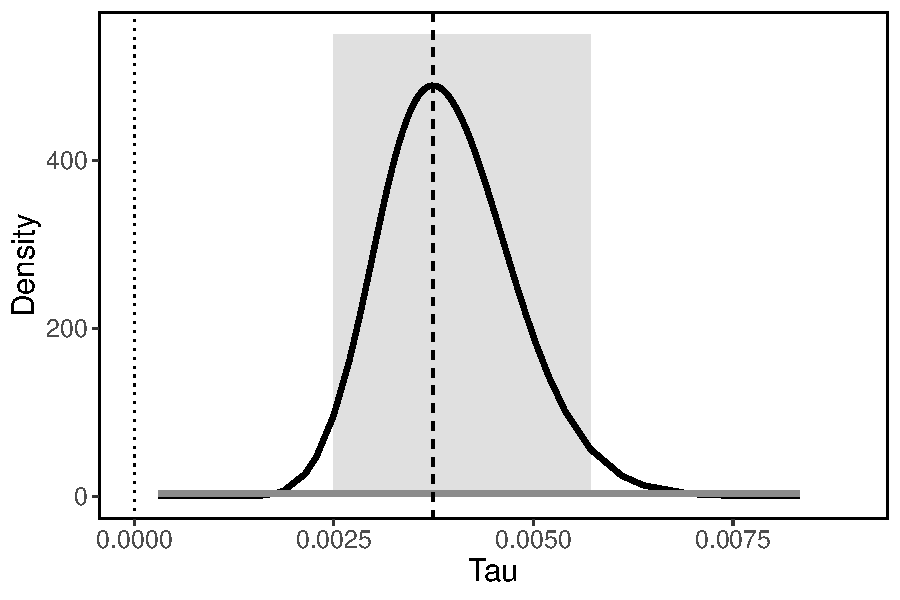
\includegraphics{Bayesian_GLMs_files/figure-latex/ch4-M0-hyp-plot-1} 

}

\caption{\textbf{Posterior and prior distributions for the precision of the hyperparameter of a Bayesian linear regression to predict the territorial response distance of male European bitterling to a rival. The model is fitted with default (non-informative) priors. The solid black line is the posterior distribution, the solid gray line is the prior distribution, the gray shaded area encompasses the 95\% credible intervals, the vertical dashed line is the posterior mode, the vertical dotted line indicates zero.}}\label{fig:ch4-M0-hyp-plot}
\end{figure}

Since we typically do not work with precision, we obtain the posterior distribution of the standard deviation of the hyperparameter (sigma, \(\sigma\)) with:

\texttt{round(bri.hyperpar.summary(M0),2)}

\begin{longtable}[]{@{}ccccc@{}}
\toprule
& mean & mode & 0.025quant & 0.975quant \\
\midrule
\endhead
SD for Gaussian observations & 16.17 & 15.69 & 13.24 & 19.97 \\
\bottomrule
\end{longtable}

Visualisation of the posterior distribution of the standard deviation of the hyperparameter can be achieved with \texttt{ggplot2} using R script associated with this chapter.



\begin{figure}

{\centering 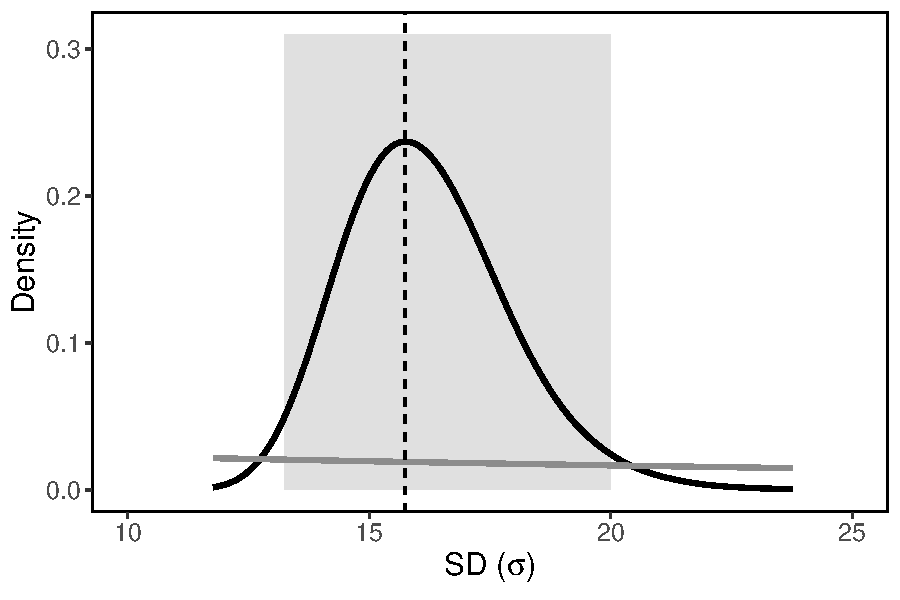
\includegraphics{Bayesian_GLMs_files/figure-latex/ch4-M0-brihyp-plot-1} 

}

\caption{\textbf{Posterior and prior distributions for the standard deviation of the hyperparameter of a Bayesian linear regression to predict the territorial response distance of male European bitterling to a rival. The model is fitted with default (non-informative) priors. The solid black line is the posterior distribution, the solid gray line is the prior distribution, the gray shaded area encompasses the 95\% credible intervals, the vertical dashed line is the posterior mode.}}\label{fig:ch4-M0-brihyp-plot}
\end{figure}

Clearly the standard deviation of the hyperparameter differs from zero (Fig. \ref{fig:ch4-M0-brihyp-plot}). The distribution is also not normal; the default prior is for a gamma distribution.

\hypertarget{model-with-informative-priors}{%
\subsubsection{Model with informative priors}\label{model-with-informative-priors}}

As for the model with default priors, we will examine the posterior distributions for the model with informative priors, starting with the fixed effects.

\hypertarget{fixed-effects-1}{%
\paragraph{Fixed effects}\label{fixed-effects-1}}

First examine the posterior mean and 95\% credible intervals for the fixed effects:

\texttt{M1Betas\ \textless{}-\ M1\$summary.fixed{[},c("mean",\ "sd",\ "0.025quant",\ "0.975quant"){]}}

\texttt{round(M1Betas,\ digits\ =\ 2)}

\begin{verbatim}
             mean    sd 0.025quant 0.975quant
(Intercept) 55.09 12.56      30.42      79.81
sl           1.84  0.24       1.37       2.31
fSupp1      41.12 12.82      15.90      66.22
sl:fSupp1   -0.24  0.26      -0.74       0.27
\end{verbatim}

This reports the posterior mean, standard deviation and 95\% credible intervals for the \texttt{intercept}, covariates (\texttt{sl}, \texttt{fSupp1}) and interaction (\texttt{sl:fSupp1}). Note that the posterior means differ quantitatively from the default model as do the 95\% credible intervals, which encompass a narrower range in each case.

For the variable \texttt{sl} we now have a posterior mean of the slope of 1.84 and lower 95\% credible interval of 1.37 and upper 95\% credible interval of 2.31. We can conclude from this result that we are 95\% certain that the posterior mean of the regression parameter for the slope of sl falls between these credible intervals, centered around the posterior mean.

We can similarly conclude that the \texttt{Intercept} of the relationship differs from zero, with a posterior mean of 55.09 and credible intervals from 30.42 to 79.81.

For supplementary feeding (\texttt{fSupp1}), in contrast to the model with non-informative priors, the parameter is statistically important, with a posterior mean of 41.12 and 95\% credible intervals from 15.9 to 66.22.

In the case of the interaction between standard length and supplementary feeding (\texttt{sl:fSupp1}) the credible intervals range from negative values for the lower interval (-0.74) to positive for the upper interval (0.27), indicating that this model parameter does not differ from zero.

The posterior distributions of the fixed effects can be visualized using ggplot2. The coding for this plot is available in the R script associated with this chapter.



\begin{figure}

{\centering 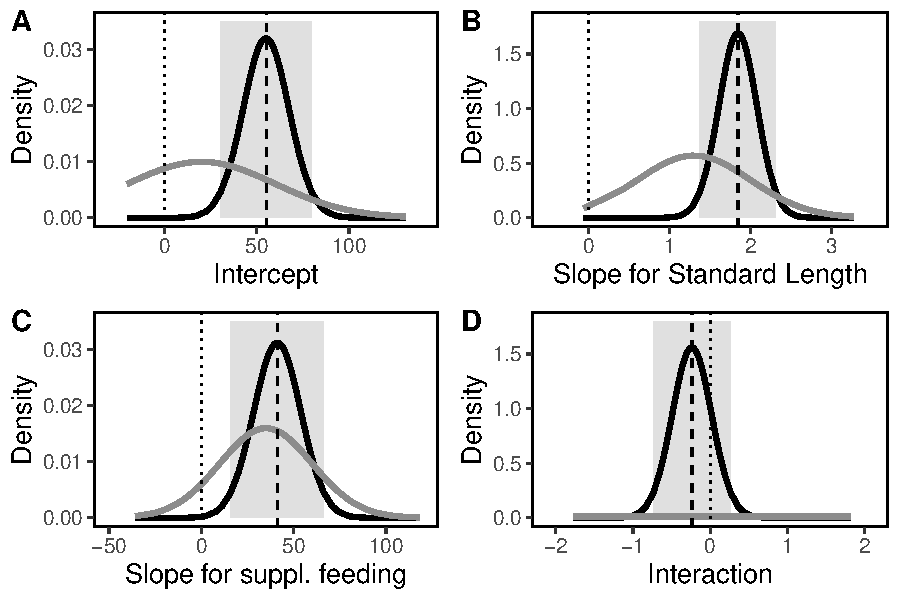
\includegraphics{Bayesian_GLMs_files/figure-latex/ch4-M1-betas-1} 

}

\caption{\textbf{Posterior and prior distributions for fixed parameters of a Bayesian linear regression to predict the territorial response distance of male European bitterling (\emph{Rhodeus amarus}) in response to a rival fitted with informative priors. Distributions for: A. model intercept; B. slope for male standard length; C. slope for supplementary feeding; D. interaction of male standard length and supplementary feeding. The solid black line is the posterior distribution, the solid gray line is the prior distribution, the gray shaded area encompasses the 95\% credible intervals, the vertical dashed line is the posterior mean of the parameter, the vertical dotted line indicates zero. For parameters where zero (indicated by dotted line) falls outside the range of the 95\% credible intervals (gray shaded area), the parameter is considered statistically important (i.e.~in the case of panels A, B and C).}}\label{fig:ch4-M1-betas}
\end{figure}

Figure \ref{fig:ch4-M1-betas} indicates that for model M1 the intercept, slope for male standard length and slope for supplementary feeding all differ from zero and are statistically important in the model. The interaction between standard length and supplementary feeding is not. This figure also shows the distributions of the informative priors, based on the pilot study described in Section \ref{pilot}. These informative priors influence the posterior distribution.

\hypertarget{hyperparameter-1}{%
\paragraph{Hyperparameter}\label{hyperparameter-1}}

A summary of the precision of the hyperparameter for the informative model is obtained with:

\texttt{M1hyp\ \textless{}-\ M1\$summary.hyper{[},c("mean",\ "mode",\ "0.025quant",\ "0.975quant"){]}}

\begin{longtable}[]{@{}ccccc@{}}
\toprule
& mean & mode & 0.025quant & 0.975quant \\
\midrule
\endhead
Precision for Gaussian obs & 0.0048 & 0.0046 & 0.0032 & 0.0066 \\
\bottomrule
\end{longtable}

The posterior distribution of the precision of the hyperparameter can be visualized using ggplot2. The coding for this plot is available in the R script associated with this chapter.



\begin{figure}

{\centering 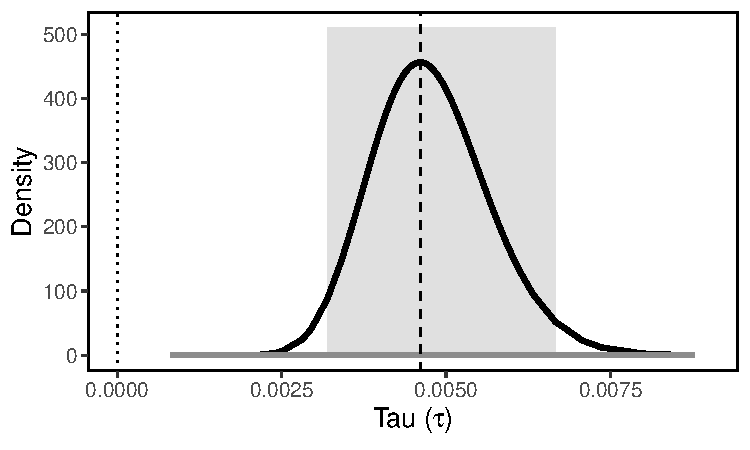
\includegraphics{Bayesian_GLMs_files/figure-latex/ch4-M1-hyp-plot-1} 

}

\caption{\textbf{Posterior distribution for the precision of the hyperparameter of a Bayesian linear regression to predict the territorial response distance of male European bitterling to a rival. The model is fitted with a weakly informative prior on the hyperparameter. The solid black line is the posterior distribution, solid gray line is the prior distribution, the gray shaded area encompasses the 95\% credible intervals, the vertical dashed line is the posterior mode, the vertical dotted line indicates zero.}}\label{fig:ch4-M1-hyp-plot}
\end{figure}

While informative priors were put on fixed effects in the model, a weakly informative prior was put on the hyperparameter; evident in the prior distribution in Fig. \ref{fig:ch4-M1-hyp-plot}. The 95\% credible intervals of the posterior distribution of the hyperparameter do not include zero.

We can obtain the posterior distribution of the standard deviation of the hyperparameter (sigma, \(\sigma\)) with:

\texttt{round(bri.hyperpar.summary(M1),2)}

\begin{longtable}[]{@{}ccccc@{}}
\toprule
& mean & mode & 0.025quant & 0.975quant \\
\midrule
\endhead
SD for Gaussian observations & 14.67 & 14.30 & 14.56 & 17.67 \\
\bottomrule
\end{longtable}

Visualisation of the posterior distribution of the standard deviation of the hyperparameter can be accomplished with \texttt{ggplot2} using R script associated with this chapter.



\begin{figure}

{\centering 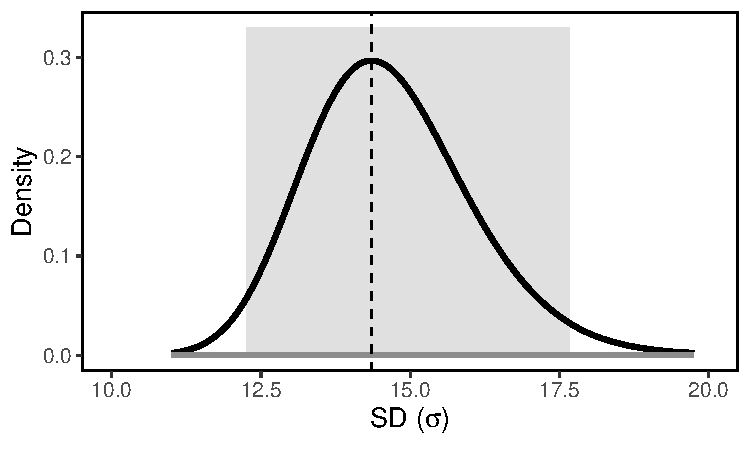
\includegraphics{Bayesian_GLMs_files/figure-latex/ch4-M1-bri-plot-1} 

}

\caption{\textbf{Posterior and prior distributions for the standard deviation of the hyperparameter of a Bayesian linear regression to predict the territorial response distance of male European bitterling to a rival. The model is fitted with a weakly informative prior on the hyperparameter. The solid black line is the posterior distribution, the solid gray line is the prior distribution, the gray shaded area encompasses the 95\% credible intervals, the vertical dashed line is the posterior mode.}}\label{fig:ch4-M1-bri-plot}
\end{figure}

\hypertarget{comparison-with-frequentist-gaussian-glm}{%
\subsubsection{Comparison with frequentist Gaussian GLM}\label{comparison-with-frequentist-gaussian-glm}}

At this stage it is instructive to compare the results of the Bayesian Gaussian GLMs with the same model fitted in a frequentist setting. Execution of the model in a frequentist framework can be performed with:

\texttt{Freq\ \textless{}-\ lm(resp\_dist\ \textasciitilde{}\ sl\ *\ fSupp,\ data\ =\ bitt)}

The results are obtained with:

\texttt{broom::tidy(Freq)\%\textgreater{}\%\ mutate\_if(is.numeric,\ round,\ 4)}

\begin{verbatim}
# A tibble: 4 x 5
  term        estimate std.error statistic p.value
  <chr>          <dbl>     <dbl>     <dbl>   <dbl>
1 (Intercept)   47.7      18.8        2.54  0.0148
2 sl             1.98      0.353      5.61  0     
3 fSupp1        59.1      28.9        2.05  0.0467
4 sl:fSupp1     -0.580     0.554     -1.05  0.301 
\end{verbatim}

We already have the results for the Bayesian models; for the model with default priors these are:

\texttt{round(M0Betas,\ digits\ =\ 2)}

\begin{verbatim}
             mean    sd 0.025quant 0.975quant
(Intercept) 59.07 17.01      25.91      92.88
sl           1.77  0.32       1.13       2.40
fSupp1      32.35 21.50     -10.41      74.11
sl:fSupp1   -0.07  0.42      -0.88       0.75
\end{verbatim}

For the Bayesian model with informative priors:

\texttt{round(M1Betas,\ digits\ =\ 2)}

\begin{verbatim}
             mean    sd 0.025quant 0.975quant
(Intercept) 55.09 12.56      30.42      79.81
sl           1.84  0.24       1.37       2.31
fSupp1      41.12 12.82      15.90      66.22
sl:fSupp1   -0.24  0.26      -0.74       0.27
\end{verbatim}

These results can be summarised together in a table:

Table 4.1: \textbf{Parameters for fixed effects of a model to investigate the effect of standard length (sl) and supplementary feeding treatment (fSupp) and their interaction on the territorial response distance of male European bitterling for a frequentist GLM, Bayesian GLM with default priors and Bayesian GLM with informative priors. Mean (sd) parameter estimates are shown for each model}

\begin{longtable}[]{@{}lcccc@{}}
\toprule
Model & Intercept & sl & fSupp & sl : fSupp1 \\
\midrule
\endhead
Frequentist & 47.7(18.8) & 2.0(0.4) & 59.1(28.9) & -0.6(0.6) \\
Bayesian (default) & 59.1(17.0) & 1.8(0.3) & 32.4(21.5) & -0.1(0.4) \\
Bayesian (informative) & 55.3(12.5) & 1.8(0.2) & 40.5(12.4) & -0.2(0.3) \\
\bottomrule
\end{longtable}

While parameter estimates for the frequentist and Bayesian models are broadly similar, it is notable that results for the Bayesian model with default (non-informative) priors diverge more from the results for the frequentist model than do the parameter estimates for the Bayesian model with informative priors.

It is a common misconception that non-informative priors are objective and provide an unbiased representation of the data. However, `non-informative' is a misnomer, because all priors influence model outcomes. In a Bayesian framework, the implementation of carefully specified informative priors will typically be more likely to generate robust results than reliance on default priors.

We can also compare the standard deviation of the residuals (sigmas) for these models.

For the Frequentist model:

\texttt{round(summary(Freq)\$sigma,2)}

16.22

For the Bayesian model with default priors:

\texttt{round(bri.hyperpar.summary(M0){[},c("mean"){]},2)}

16.19

For the Bayesian model with informative priors:

\texttt{round(bri.hyperpar.summary(M1){[},c("mean"){]},2)}

14.67

Estimates of sigma are almost identical for the frequentist and Bayesian model with default priors. The greater precision of the Bayesian model with informative priors is reflected by a smaller sigma.

\hypertarget{conduct-model-checks}{%
\subsection{Conduct model checks}\label{conduct-model-checks}}

After model fitting and obtaining the posterior distributions, an important next step is validation of the model through model checks. At this stage we may also wish to perform model selection.

\hypertarget{model-selection-using-the-deviance-information-criterion-dic}{%
\subsubsection{Model selection using the Deviance Information Criterion (DIC)}\label{model-selection-using-the-deviance-information-criterion-dic}}

When a model is fitted with several explanatory variables, including interaction terms, we have the opportunity to conduct \emph{model selection}. Model selection involves finding an optimal set of covariates for a model. It is a hotly debated subject in statistics, with several alternative approaches. Here we present a simple model selection procedure for models \texttt{M0} and \texttt{M1}. A more sophisticated model selection procedure using an Information Theoretic (IT) approach is presented in Chapter 5.

In a frequentist setting a common approach to model selection is to use classical backward or forward stepwise model selection based on the Akaike Information Criteria (AIC). AIC measures goodness-of-fit and model complexity, with the lower the AIC score, the better the fit of the model to the data, penalised by model complexity. In backward model selection, a model with all covariates is fitted and then sequential deletion of covariates is undertaken until removal of further covariates fails to improve the fit of the model. In forward selection this procedure is reversed.

In a Bayesian framework the Deviance Information Criterion (DIC) can similarly be used to compare model goodness-of-fit while penalising model complexity. Like AIC, a smaller DIC score indicates a better fit of the model to the data given its complexity.

A model's DIC score can be computed in INLA using the \texttt{dic\ =\ TRUE} option in \texttt{control.compute}. For model \texttt{M0}:

\texttt{M0\ \textless{}-\ inla(resp\_dist\ \textasciitilde{}\ sl\ *\ fSupp,\ control.compute\ =\ list(dic\ =\ TRUE),\ data\ =\ bitt)}

And the same can be computed for \texttt{M1}.

For \texttt{INLA} there is no stepwise model selection procedure (such as the \texttt{drop1} and \texttt{step} functions for frequentist GLMs), which means model selection must be conducted manually.

The goal in conducting model selection in this case is twofold:

\begin{enumerate}
\def\labelenumi{\arabic{enumi}.}
\item
  Compare full and reduced models for models with non-informative and informative priors.
\item
  Compare best-fitting models with non-informative and informative priors.
\end{enumerate}

Start by sequentially removing model parameters from \texttt{M0} and then compare using the DIC:

The full model:

\texttt{M0.full\ \textless{}-\ inla(resp\_dist\ \textasciitilde{}\ sl\ *\ fSupp,\ control.compute\ =\ list(dic\ =\ TRUE),\ data\ =\ bitt)}

Drop interaction:

\texttt{M0.1\ \textless{}-\ inla(resp\_dist\ \textasciitilde{}\ sl\ +\ fSupp,\ control.compute\ =\ list(dic\ =\ TRUE),\ data\ =\ bitt)}

Drop supplementary feeding:

\texttt{M0.2\ \textless{}-\ inla(resp\_dist\ \textasciitilde{}\ sl,\ control.compute\ =\ list(dic\ =\ TRUE),\ data\ =\ bitt)}

Drop standard length:

\texttt{M0.3\ \textless{}-\ inla(resp\_dist\ \textasciitilde{}\ fSupp,\ control.compute\ =\ list(dic\ =\ TRUE),\ data\ =\ bitt)}

Compare with the DIC:

\texttt{DIC\ \textless{}-\ cbind(c(M0.full\$dic\$dic,\ M0.1\$dic\$dic,\ M0.2\$dic\$dic,\ \ \ \ M0.3\$dic\$dic))}
\texttt{rownames(DIC)\ \textless{}-\ c("full","no\ inter","no\ suppl","no\ sl")}
\texttt{round(DIC,1)}

\begin{verbatim}
           DIC
full     409.7
no inter 408.9
no suppl 436.6
no sl    438.0
\end{verbatim}

The model without an interaction generates the lowest DIC score (408.9). This score is only marginally lower than the score for the full model with the interaction included, which is an indication that the interaction is not important in the model. A difference in DIC scores of between 5 and 10 would be considered substantial.

Following the same procedure with model M1 (see R script associated with this chapter) yields:

\begin{verbatim}
           DIC
full     408.4
no inter 408.5
no suppl 436.7
no sl    438.2
\end{verbatim}

In this case the full model, with an interaction, generates the lowest DIC score (408.4). However, as in the case above, this score is only marginally lower than the score for the model without the interaction, which tells us that the interaction is not important.

We can conclude that both for the model with non-informative and informative priors that the best-fitting model in each case is the one that includes both \texttt{sl} and \texttt{fSupp}, but with no interaction between them.

We can now compare the best-fitting models with non-informative and informative priors using the DIC:

\texttt{DIC2\ \textless{}-\ cbind(c(M0.1\$dic\$dic,\ M1.1\$dic\$dic))}

\texttt{rownames(DIC2)\ \textless{}-\ c("default\ priors","informative\ priors")}

\texttt{colnames(DIC2)\ \textless{}-\ "DIC"}

\texttt{round(DIC2,2)}

\begin{verbatim}
                      DIC
default priors     408.92
informative priors 408.47
\end{verbatim}

These DIC score are essentially the same.

Given the similarity in goodness-of-fit of both these models, what should we do? Since the DIC scores for both models are essentially the same, the appropriate course is to continue with model checking for both and present the findings for both models. For brevity, however, we will continue by examining the model with informative priors only.

\hypertarget{posterior-predictive-checks}{%
\subsubsection{Posterior predictive checks}\label{posterior-predictive-checks}}

The purpose of posterior predictive checks is to assess if a model generates realistic predictions. It does this by drawing simulated estimates from the joint posterior predictive distribution and comparing them with observed data. Any departure of the simulated data from the observed data will reflect problems with the model. Ideally, simulated data should match the observed. This matching is performed with a posterior predictive p-value. If the posterior predictive p-value is close to 0.5 it means simulated and observed data are similar. However, if a posterior predictive p-value is close to 1 it means the model prediction is too high, if close to zero, the model prediction is too low. A frequency plot of posterior predictive p-values should show a distribution centred around 0.5.

In \texttt{INLA} the posterior predictive p-value can be obtained with the function \texttt{inla.pmarginal()}. See the R script associated with this chapter for estimating and plotting the posterior predictive p-values for the Bayesian model with informative priors without interaction.



\begin{figure}

{\centering 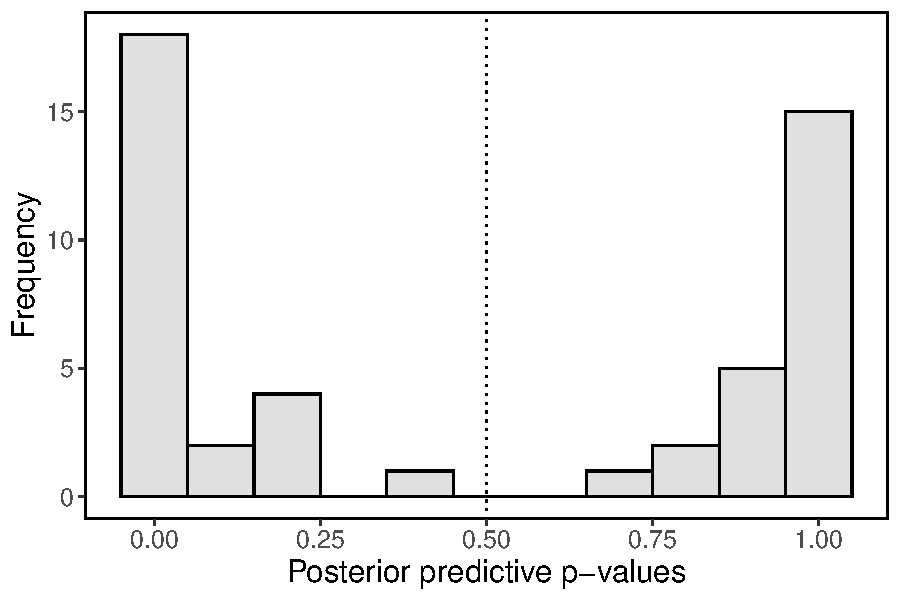
\includegraphics{Bayesian_GLMs_files/figure-latex/ch4-post-p-1} 

}

\caption{\textbf{Frequency histogram of the posterior predictive p-values for the best-fitting Bayesian linear regression with informative priors to predict the territorial response distance of male European bitterling to a rival. The vertical dotted line indicates 0.5.}}\label{fig:ch4-post-p}
\end{figure}

The frequency histogram of posterior predictive p-values in Fig. \ref{fig:ch4-post-p} shows that most values are close to zero or 1, with few close to 0.5, which indicates the model check has not been satisfied; the data are overdispersed compared to the model. Consequently, we will proceed with further model checks.

\hypertarget{cross-validation-model-checking}{%
\subsubsection{Cross-validation model checking}\label{cross-validation-model-checking}}

Cross validation is a model-checking approach that examines how well a model is able to generalise to new data. Leave-one-out cross validation (LOO-CV) involves systematically dropping a single data point, refitting the model and evaluating the altered model inference. Following \citep{Wang_2018}, we use the \emph{conditional predictive ordinate} (CPO) and \emph{probability integral transform} (PIT) to evaluate model goodness-of-fit. To obtain both we simply run the model using the \texttt{cpo\ =\ TRUE} option in \texttt{control.compute}.

To ensure there are no potential numerical problems in estimating CPO or PIT for a given model, we first run the following check:

\texttt{sum(M1.pred\$cpo\$failure)}

0

An outcome of zero indicates no problems with the computation of CPO or PIT. A value of 1 would indicate CPO or PIT were unreliable.

Plotting PIT values will indicate whether the predictive distributions match the data, apparent as a uniform distribution. We can assess uniformity visually with a frequency histogram and Q-Q plot of PIT values for a uniform distribution (see the R script associated with this chapter).



\begin{figure}

{\centering 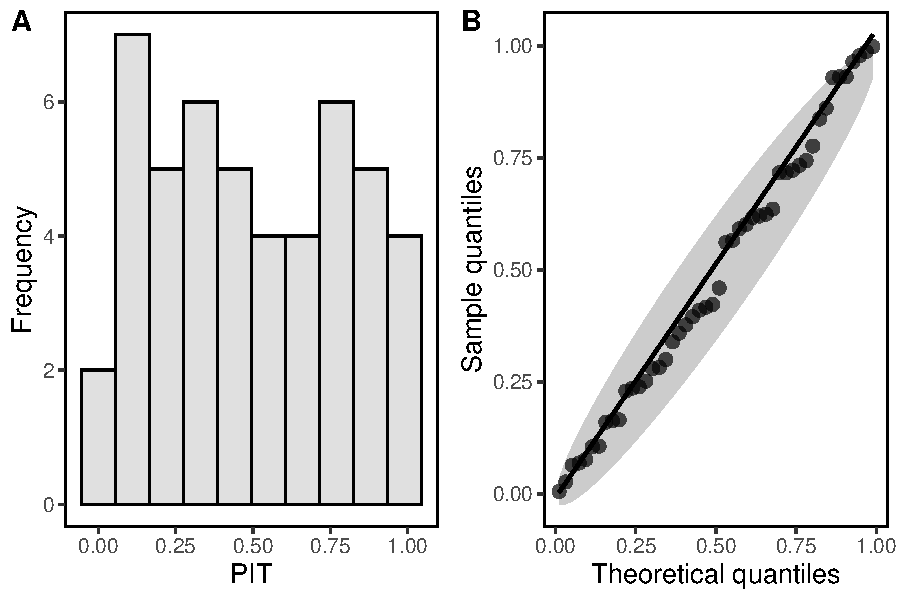
\includegraphics{Bayesian_GLMs_files/figure-latex/ch4-PIT-1} 

}

\caption{\textbf{A. Frequency histogram; B. Uniform Q-Q plot with confidence bands (shaded gray), for cross-validated probability integral transform (PIT) values for the best-fitting Bayesian linear regression with informative priors.}}\label{fig:ch4-PIT}
\end{figure}

The frequency histogram of PIT values in Fig. \ref{fig:ch4-PIT} A shows that the distribution is broadly uniform, with no clustering of values at zero or 1. This conclusion is supported by the Q-Q plot (Fig. \ref{fig:ch4-PIT} B), which shows that the PIT values match a uniform distribution.

\hypertarget{bayesian-residuals-analysis}{%
\subsubsection{Bayesian residuals analysis}\label{bayesian-residuals-analysis}}

Homogeneity of residual variance can be assessed visually by plotting model residual variance against fitted values as well as each variable in the model (see the R script associated with this chapter).



\begin{figure}

{\centering 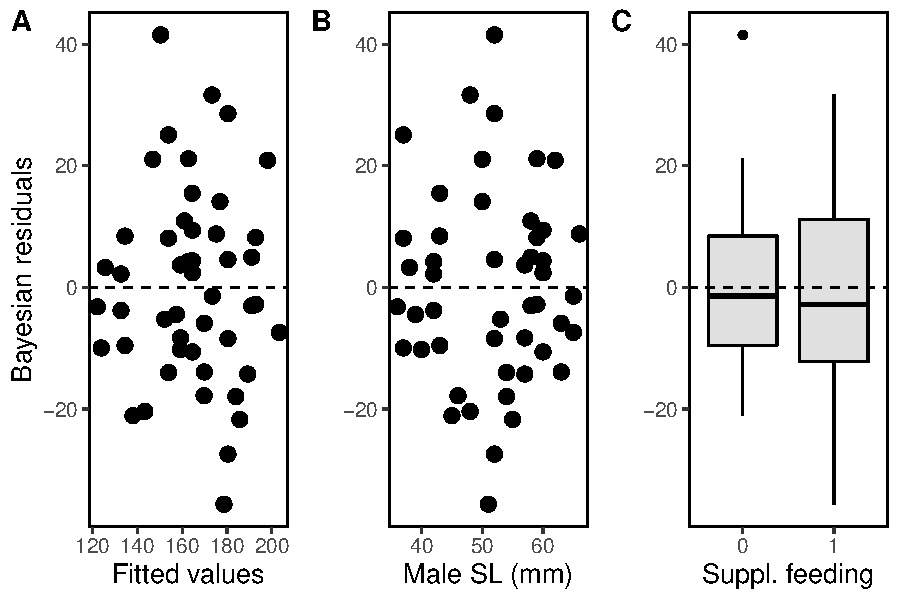
\includegraphics{Bayesian_GLMs_files/figure-latex/ch4-resids-1} 

}

\caption{\textbf{Bayesian residuals plotted against: A. fitted values ; B. male standard length; and C. supplementary feeding, to assess homogeneity of residual variance.}}\label{fig:ch4-resids}
\end{figure}

Ideally, the distribution of residuals around zero should be random along the horizontal axis, which is the case in Fig. \ref{fig:ch4-resids} A and B, and in the case of a categorical variable, the median of a boxplot of residual values should be approximately zero, which is the case in Fig. \ref{fig:ch4-resids} C.

\hypertarget{prior-sensitivity-analysis}{%
\subsubsection{Prior sensitivity analysis}\label{prior-sensitivity-analysis}}

A final Bayesian model check is to examine prior distributions through a sensitivity analysis. This procedure is important both in the case of non-informative and informative priors. The procedure involves systematically changing prior distributions and examining the magnitude of outcome for the posterior distribution.

To investigate the impact of different priors, we increased and decreased priors on the fixed effects by 20\% and examined the outcome for the posterior mean.

The original priors for the fixed effects were:

\(\beta intercept\) \textasciitilde{} \emph{N}(20, 1600)

\(\beta sl\) \textasciitilde{} \emph{N}(1.3, 0.49)

\(\beta fSupp1\) \textasciitilde{} \emph{N}(35, 225)

In the case of an increase by 20\%, the priors for the fixed effects are:

\(\beta intercept\) \textasciitilde{} \emph{N}(24, 1920)

\(\beta sl\) \textasciitilde{} \emph{N}(1.56, 0.59)

\(\beta fSupp1\) \textasciitilde{} \emph{N}(42, 270)

In the case of a decrease by 20\%, the priors for the fixed effects are:

\(\beta intercept\) \textasciitilde{} \emph{N}(16, 1280)

\(\beta sl\) \textasciitilde{} \emph{N}(1.04, 0.39)

\(\beta fSupp1\) \textasciitilde{} \emph{N}(28, 180)

Two alternative models were fitted with these increases and decreases in the priors and estimates for the betas obtained (see the R script associated with this chapter).

Table 4.2: \textbf{Sensitivity analysis for a 20\% increase and decrease in priors on fixed effects and the \% change in the posterior mean.}

\begin{longtable}[]{@{}lccccc@{}}
\toprule
Parameter & \% prior & Mean & 0.025CI & 0.975CI & \% posterior \\
\midrule
\endhead
& +20 & 57.6 & 33.5 & 81.5 & -1.68 \\
Intercept & 0 & 58.6 & 34.9 & 82.1 & 0 \\
& -20 & 60.0 & 37.0 & 83.0 & 2.44 \\
& & & & & \\
& +20 & 1.8 & 1.3 & 2.2 & 0.92 \\
sl & 0 & 1.8 & 1.3 & 2.2 & 0 \\
& -20 & 1.7 & 1.3 & 2.2 & -1.35 \\
& & & & & \\
& +20 & 30.3 & 22.2 & 38.5 & 1.18 \\
fSupp1 & 0 & 30.0 & 21.9 & 38.1 & 0 \\
& -20 & 29.4 & 21.4 & 37.5 & -1.69 \\
\bottomrule
\end{longtable}

The results of the prior sensitivity analysis show that changes as large as 20\% (increase and decrease) result in negligible changes to the posterior distribution.

We can plot the posterior distributions of these alternative models to visualise the changes (see R script associated with this chapter).



\begin{figure}

{\centering 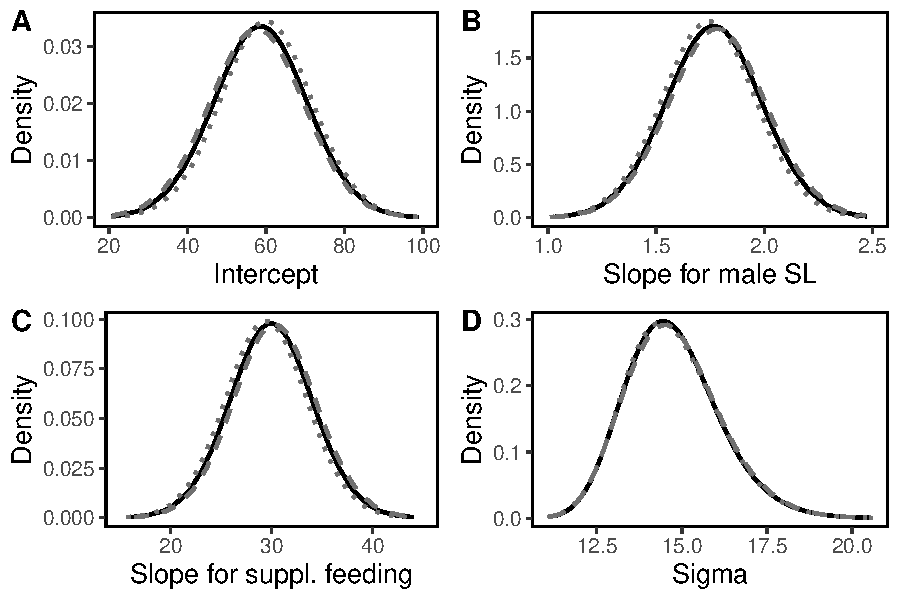
\includegraphics{Bayesian_GLMs_files/figure-latex/ch4-plot-pos-1} 

}

\caption{\textbf{Posterior distributions for parameters of a Bayesian linear regression to predict the territorial response distance of male European bitterling in response to a rival. Distributions for: A. model intercept; B. slope for male standard length; C. slope for supplementary feeding; D. hyperparameter. The solid black line is the posterior distribution for the optimal model, the dashed gray line is the posterior distribution for an alternative model with the priors increased by 20\%, the dotted gray line is the posterior distribution for an alternative model with the priors decreased by 20\%.}}\label{fig:ch4-plot-pos}
\end{figure}

Plots of the posterior distributions for the fixed effects and hyperparameter (Fig. \ref{fig:ch4-plot-pos}) further illustrate that the posterior distributions of model parameters are robust to changes in the priors.

\hypertarget{conclusions-from-model-checks}{%
\subsubsection{Conclusions from model checks}\label{conclusions-from-model-checks}}

Manual model selection based on the DIC allowed us to slightly refine the model by dropping the interaction between male standard length and the provision of supplementary food. The model with informative priors showed a comparable goodness-of-fit to that of the model with default priors. A plot of posterior predictive p-values suggested some overdispersion of the model, though leave-one-out cross validation indicated that the predictive distributions matched the data well. Residuals plots failed to highlight anything problematic with the model fit. Prior sensitivity analysis demonstrated the model to be robust to changes in prior distributions of fixed effects. Overall, then, the Bayesian GLM with informative priors appears to provide a good representation of the data.

\hypertarget{interpret-and-present-model-output}{%
\subsection{Interpret and present model output}\label{interpret-and-present-model-output}}

We specify the Bayesian GLM using mathematical notation in exactly the same way as we would for a frequentist model:

\(Response_{i}\) \textasciitilde{} \(Gaussian(\mu_{i}\), \(\sigma^{2})\)

\emph{E}(\(Response_i\)) = \(\mu_i\) and var(\(Response_{i}\)) = \(\sigma^{2}\)

\(\mu_{i}\) = \(\beta_1\) + \(\beta_2\) x \(Length_{i}\) + \(\beta_3\) x \(Supplement_{i}\)

Where \(Response_{i}\) is the aggressive response distance (cm) of male European bitterling \emph{i} assuming a normal distribution with mean \(\mu_{i}\) and variance \(\sigma^{2}\). \(Length_{i}\) is a continuous covariate representing the standard length of male bitterling \emph{i} (mm) and \(Supplement_{i}\) is a categorical variable representing the provision of supplementary food to male \emph{i}, with two levels; supplement provided or no supplement. The numerical output for the fixed effects of the final model is:

\begin{verbatim}
             mean    sd 0.025quant 0.975quant
(Intercept) 58.56 12.01      34.88      82.11
sl           1.77  0.22       1.33       2.21
fSupp1      29.95  4.12      21.87      38.08
\end{verbatim}

And for sigma:

\begin{verbatim}
      mean   q0.025   q0.975  term
1 14.73564 12.33454 17.73963 sigma
\end{verbatim}

These results can be more formally presented in the following way:

Table 4.3: \textbf{Posterior mean estimates for aggressive response distances (cm) of male European bitterling (\emph{Rhodeus amarus}) as a function of male standard length (mm) and a supplementary feeding treatment, modelled using a Gaussian GLM fitted using Bayesian inference with INLA. CrI are the Bayesian 95\% credible intervals.}

\begin{longtable}[]{@{}lccc@{}}
\toprule
Model parameter & Posterior mean & Lower 95\% CrI & Upper 95\% CrI \\
\midrule
\endhead
Intercept & 58.56 & 34.92 & 82.09 \\
Standard length & 1.77 & 1.33 & 2.21 \\
Supplementary feeding & 29.25 & 21.88 & 38.07 \\
\(\sigma\) & 14.75 & 12.32 & 17.75 \\
\bottomrule
\end{longtable}

These results show a statistically important positive effect of male bitterling standard length on response distance, with larger males initiating attacks on a rival at greater distances than smaller males. The effect of supplementary feeding for 6-days prior to testing was similarly to increase the aggressive response distance to a rival.

\hypertarget{visualise-the-results}{%
\subsection{Visualise the results}\label{visualise-the-results}}

The final of the 9 steps to fitting a Bayesian GLM is to visualise the model (Section \ref{glm-steps}). A figure helps with understanding model outcomes and is a valuable summary of the model findings for a paper, thesis or report. The full coding for this plot is available in the R script associated with this chapter.

We start by defining a dataframe (`\texttt{MyData}') that contains \texttt{sl} and \texttt{fSupp} using \texttt{dplyr} functions:

\texttt{MyData\ \textless{}-\ ddply(bitt,\ .(fSupp),\ summarize,\ sl\ =\ seq(from\ =\ min(sl),\ to\ =\ max(sl),\ length\ =\ 50))}

This creates 100 artificial covariate values. There is no \texttt{predict} function in INLA, but we can obtain fitted values manually with a design matrix for the values in \texttt{MyData} and then multiply this with the posterior mean values of the model.

We must also add an extra variable for the response variable to \texttt{MyData} and assign it `NA'. We will then combine the \texttt{bitt} and \texttt{MyData} objects, and apply INLA to this combined data set. INLA will predict the response variable where an NA occurs.

\texttt{MyData\$resp\_dist\ \textless{}-\ NA}

\texttt{bitt.Pred\ \textless{}-\ bitt{[},\ colnames(MyData){]}}

\texttt{bitt.Comb\ \textless{}-\ rbind(bitt.Pred,\ MyData)}

We next re-run the model in \texttt{INLA} using the combined data set (\texttt{bitt.Comb}), ensuring that \texttt{compute\ =\ TRUE} is selected in the \texttt{control.predictor} argument:

\texttt{Final.Pred\ \textless{}-\ inla(resp\_dist\ \textasciitilde{}\ sl\ +\ fSupp,\ \ data\ =\ bitt.Comb,\ control.predictor\ =\ list(compute\ =\ TRUE),\ control.family\ =\ list(hyper\ =\ list(prec\ =\ list(prior\ =\ "gaussian",param\ =\ c(0,1)))),\ control.fixed\ =\ list(mean.intercept\ =\ 20,\ prec.intercept\ =\ 40\^{}(-2),\ mean\ =\ list(sl\ =\ 1.3,\ fSupp1\ =\ 35,\ default\ =\ 0),\ prec\ =\ list(sl\ =\ 0.7\^{}(-2),\ fSupp1\ =\ 15\^{}(-2),\ default\ =\ 1000)))}

Generate predicted values and relevant components in \texttt{MyData}

\texttt{Pred\ \textless{}-\ Final.Pred\$summary.fitted.values{[}((nrow(bitt))+1):\ (nrow(bitt)\ +\ nrow(MyData)),{]}}

\texttt{MyData\$mu\ \ \ \ \textless{}-\ Pred{[},"mean"{]}}

\texttt{MyData\$selow\ \textless{}-\ Pred{[},"0.025quant"{]}}

\texttt{MyData\$seup\ \ \textless{}-\ Pred{[},"0.975quant"{]}}

Create figure labels:

\texttt{label\_supp\ \textless{}-\ c("0"\ =\ "No\ food\ supplement",\ "1"\ =\ "With\ food\ supplement")}

And plot with \texttt{ggplot2} (see the R script associated with this chapter).



\begin{figure}

{\centering 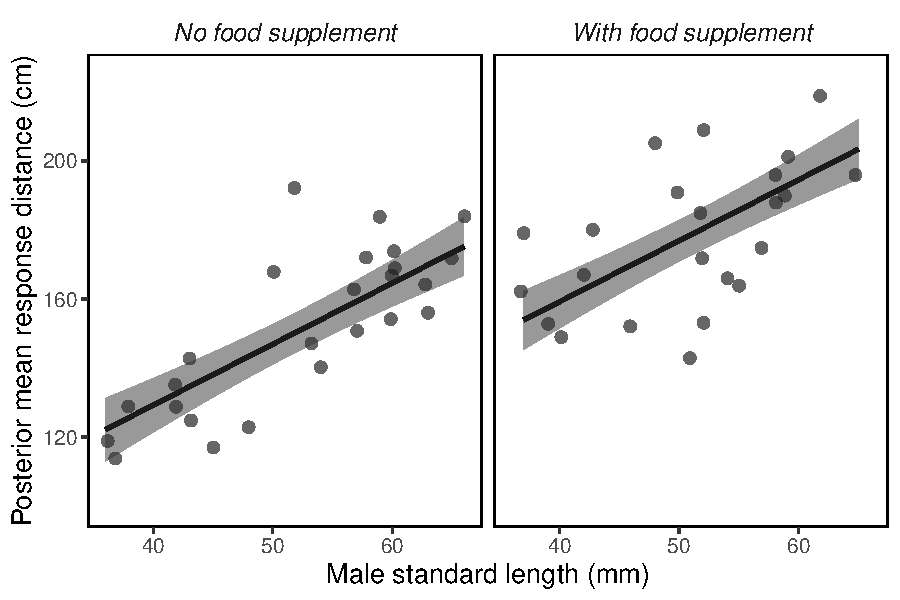
\includegraphics{Bayesian_GLMs_files/figure-latex/ch4-final-plot-1} 

}

\caption{\textbf{Posterior mean aggressive response distance (cm) of male European bitterling (\emph{Rhodeus amarus}) as a function of male standard length (mm) and supplementary feeding, modelled using a Gaussian GLM fitted using Bayesian inference with INLA. Shaded areas are Bayesian 95\% credible intervals. Black points are observed data for different males.}}\label{fig:ch4-final-plot}
\end{figure}

The results of this statistical analysis can be summarised as follows:

\emph{A Gaussian GLM was fitted to data using Bayesian inference with INLA to model the aggressive response distance (in cm) of a group of 48 territorial male European male bitterling} (Rhodeus amarus) \emph{to a model rival. There was a statistically important positive effect of male standard length (in mm) and supplementary feeding on response distance (Fig. \ref{fig:ch4-final-plot}). The mean slope of the relationship between response distance (cm) and standard length (mm) was 1.77 with 95\% certainty that it lay between 1.33 and 2.21 (Table 4.3). The effect of supplementary feeding for six days prior to testing was to increase male response distance by 30 cm, with 95\% certainty that it lay between 22 and 38 cm (Table 4.3). The model was fitted using informative priors on the fixed effects, obtained from a separate pilot study, and weakly informative effects on the hyperparameter.}

\hypertarget{conclusions-1}{%
\section{Conclusions}\label{conclusions-1}}

Bayesian inference offers an alternative approach to data analysis and has a number of advantages. One is that prior information can be incorporated into an analysis. Using prior information in a model is intuitively appealing and better reflects the scientific method of building on previous knowledge. A second advantage is in avoiding hypothesis testing and P-values, which do not allow us to draw direct conclusions about model parameters -- only about hypothetical datasets (that we will never collect). Finally, there is a large range of advanced statistical methods that can only be performed in a Bayesian setting.

While a Bayesian model adds a layer of complexity to model fitting, since a careful consideration of the priors to be used is needed, it also adds an extra dimension to the sophistication of the analysis since, instead of simply presenting a model that describes the data, we now have a mechanism for incorporating previous knowledge or expert opinion through the prior distributions we put on model parameters.

Finally, the GLM fitted here using \texttt{INLA} demonstrates the user-friendliness of this package, as well as its flexibility, repeatability and computational speed in comparison with MCMC.

\hypertarget{pois-glm}{%
\chapter{Bayesian Poisson GLM}\label{pois-glm}}

The Bayesian General Linear Model presented in Chapter 4 assumes that the response variable approximately follows a normal distribution at each level of the covariate values. Generalised linear models are a larger class of models that represent an extension of the general linear model and allow the specification of models with response variables that follow non-Gaussian distributions.

Generalised Linear Models offer the opportunity to model a much greater range of data and remove the need to transform our data to fit a normal distribution. Unfortunately the terminology around these models is confusing. The abbreviation GLM usually refers to General Linear Models; i.e.~linear regression models for a continuous response variable with continuous and/or categorical covariates. Generalised Linear Models are sometimes abbreviated as GLIM and occasionally GLZM though, confusingly, it is more typical to abbreviate them just as GLM.

We use `GLM' for both General and Generalised Linear Models, but always with a qualifying prefix. So, General Linear Models are referred to as Gaussian GLMs, while for Generalised Linear Models we specify the distribution used, such as Poisson GLM, gamma GLM, binomial GLM, etc.

In this chapter we present the first in a series of Bayesian Generalised Linear Models, starting with a Poisson GLM. A Poisson GLM is appropriate for data in which the dependent variable comprises count data. Data must not take values below zero and the variance is assumed to equal the mean.

\hypertarget{ga-plate}{%
\section{Stickleback lateral plate number}\label{ga-plate}}

In this Chapter we fit a Poisson GLM to data on lateral plate number of three-spined sticklebacks (\emph{Gasterosteus aculeatus}) from the island of North Uist in the Scottish Hebrides. Unlike most bony fishes, three-spined sticklebacks lack scales and instead possess a row of bony lateral plates along their body which, along with bony dorsal spines and pelvic girdle and pelvic spines represents `armour' that serves to protect them from predatory birds and fish. Three-spined sticklebacks show variation in the development of their bony armour and have been the focus of numerous ecological and evolutionary studies. On North Uist, populations of three-spined sticklebacks exhibit extreme variation in the development of the lateral plates, spines and pelvis, including the complete loss of these skeletal structures.

Here we analyse data on lateral plate numbers for sticklebacks from 57 populations from North Uist, along with a range of ecological variables for each population, to understand what ecological processes drive variation in armour evolution.

\emph{\textbf{Import data}}

Data for North Uist three-spined sticklebacks are saved in a comma-separated values (CSV) file \texttt{stickleback.csv} and are imported into a dataframe in R using the command:

\texttt{ga\ \textless{}-\ read\_csv(file\ =\ "stickleback.csv")}

Assess the size of the dataframe and the variables it comprises:
\texttt{str(ga)}

\begin{verbatim}
spec_tbl_df [57 x 10] (S3: spec_tbl_df/tbl_df/tbl/data.frame)
 $ loch : chr [1:57] "atan" "bhpa" ...
 $ dist : num [1:57] 0.68 1.11 1.6 0.35 0.04 ...
 $ alt  : num [1:57] 13 8 8 4 3 ...
 $ area : num [1:57] 0.08 0.53 0.36 0.44 0.41 ...
 $ ph   : num [1:57] 5.9 6 5.5 6.6 8.4 ...
 $ comp : chr [1:57] "no" "no" ...
 $ inve : chr [1:57] "no" "no" ...
 $ vert : chr [1:57] "yes" "yes" ...
 $ sl   : num [1:57] 30 30.7 30.4 28.1 41.5 ...
 $ plate: num [1:57] 1 1 0 1 8 ...
 - attr(*, "spec")=
  .. cols(
  ..   loch = col_character(),
  ..   dist = col_double(),
  ..   alt = col_double(),
  ..   area = col_double(),
  ..   ph = col_double(),
  ..   comp = col_character(),
  ..   inve = col_character(),
  ..   vert = col_character(),
  ..   sl = col_double(),
  ..   plate = col_double()
  .. )
\end{verbatim}

The dataframe comprises 57 observations of 10 variables. Each row in the dataframe represents a separate North Uist freshwater lake or \emph{loch} (\texttt{loch}). There are four continuous ecological variables: \texttt{dist} is the horizontal distance from each loch to the nearest marine habitat (in km), \texttt{alt} is the altitude of the loch above sea level (in m), \texttt{area} is the surface area of the loch (in km\textsuperscript{2}), and \texttt{pH} is loch water pH. There are also three categorical ecological variables, scored as either `yes' or `no': \texttt{comp} is the presence in a loch of nine-spined sticklebacks (\emph{Pungitius pungitius}), which are competitors of three-spined sticklebacks, \texttt{inve} is the presence of invertebrate predators of three-spined sticklebacks (primarily dragonfly and beetle larvae), and \texttt{vert} is the presence of vertebrate predators of three-spined sticklebacks (brown trout, \emph{Salmo trutta}). Two further variables are \texttt{sl}, which is the mean body length of three-spined sticklebacks from a sample of 30 fish from each loch, and \texttt{plate} is the median lateral plate number of the same 30 fish. Lateral plate number is the response variable of interest.

\hypertarget{pois-glm-steps}{%
\section{Steps in fitting a Bayesian GLM}\label{pois-glm-steps}}

We will follow the 9 steps to fitting a Bayesian GLM, detailed in Chapter 2.

\emph{1. State the question}

\emph{2. Perform data exploration}

\emph{3. Select a statistical model}

\emph{4. Specify and justify a prior distribution on parameters}

\emph{5. Fit the model}

\emph{6. Obtain the posterior distribution}

\emph{7. Conduct model checks}

\emph{8. Interpret and present model output}

\emph{9. Visualise the results}

\hypertarget{ga-question}{%
\subsection{State the question}\label{ga-question}}

This study was conducted to understand variation in lateral plate number of three-spined sticklebacks among freshwater lochs on North Uist. The topic of lateral plate evolution has been the subject of many studies over several decades, and so there are multiple hypotheses that we might investigate with these data; indeed all the ecological variables measured have previously been invoked as predictors of lateral plate evolution in three-spined sticklebacks.

This multiplicity of existing research presents us with the opportunity to compare among previous hypotheses and examine which is best supported by our data. This approach to hypothesis testing is termed an `information theory (IT) approach' and is fundamentally Bayesian, since we take prior information and update it with new data to draw the most parsimonious conclusion.

We start by formulating a set of biologically plausible alternative models comprising variables proposed as environmental agents of selection in previous studies on lateral plate number (Table 5.1).

Table 5.1: \textbf{\emph{A priori} models for the evolution of lateral plates of three-spined sticklebacks (\emph{Gasterosteus aculeatus}) in freshwater lochs on North Uist, Scotland.}

\begin{longtable}[]{@{}lll@{}}
\toprule
Model & Formulation & Source \\
\midrule
\endhead
M01 & \texttt{vert} & \citet{Morris_1956} \\
M02 & \texttt{ph} & \citet{Giles_1983} \\
M03 & \texttt{inve} & Reimchen (1994) \\
M04 & \texttt{alt} + \texttt{dist} & \citet{RAEYMAEKERS_2006} \\
M05 & \texttt{alt} + \texttt{area} & \citet{Lucek_2016} \\
M06 & \texttt{comp} & \citet{MacColl_2012} \\
M07 & \texttt{vert} + \texttt{ph} & \citet{Spence_2013} \\
M08 & \texttt{vert} + \texttt{comp} & \citet{Magalhaes_2016} \\
M09 & \texttt{ph} + \texttt{sl} & \citet{Smith_2020} \\
\bottomrule
\end{longtable}

\hypertarget{ga-eda}{%
\subsection{Data exploration}\label{ga-eda}}

We start by conducting a data exploration to identify any potential problems with the data. First check for missing data.

\texttt{colSums(is.na(ga))}

\begin{verbatim}
 loch  dist   alt  area    ph  comp  inve  vert    sl plate 
    0     0     0     0     0     0     0     0     0     0 
\end{verbatim}

There are no missing data.

\hypertarget{ga-outliers}{%
\subsubsection{Outliers}\label{ga-outliers}}

Outliers in the data can identified visually, R code for a plot of outliers is available in the R script associated with this chapter:



\begin{figure}

{\centering 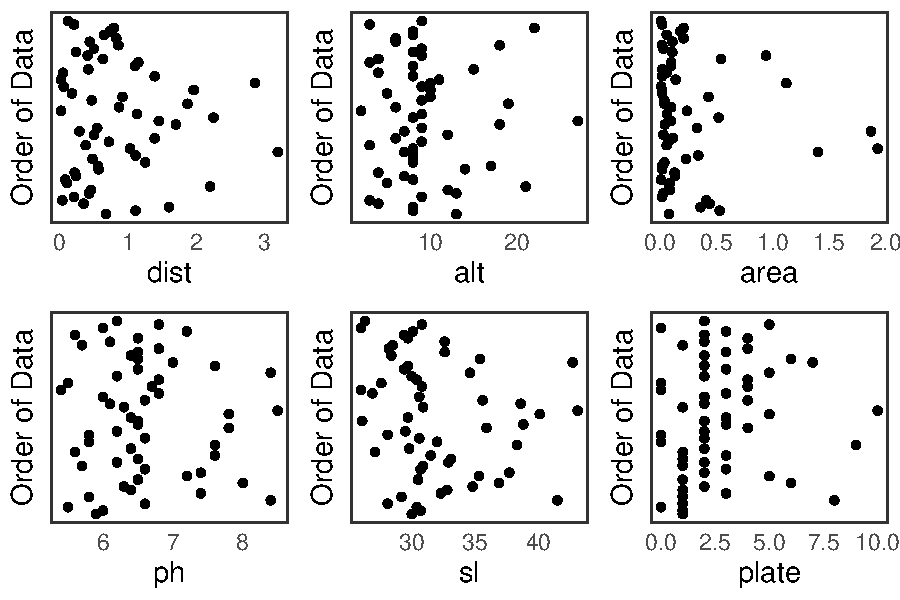
\includegraphics{Bayesian_GLMs_files/figure-latex/ch5-dotplot-1} 

}

\caption{\textbf{Dotplots of loch pH (\texttt{ph}), mean standard length (\texttt{sl}), lateral plate number (\texttt{plate}), distance to the marine environment (\texttt{dist}), altitude (\texttt{alt}) and surface area (\texttt{area}) of three-spined stickleback populations on North Uist. Data are arranged by the order they appear in the dataframe.}}\label{fig:ch5-dotplot}
\end{figure}

There are no obvious outliers in Fig. \ref{fig:ch5-dotplot}. However, the distribution of data for loch areas is clumped, indicating a large number of small lochs and a few much larger lochs. To improve the distribution of these data we can conduct a transformation of the covariate. While transformation of the response variable is to be avoided, transformation of covariates can serve to facilitate model fitting. Here we apply a log10 transformation:

\texttt{ga\$log\_area\ \textless{}-\ log10((ga\$area))}

The improvement in the distribution of the data after transformation is clear from Fig. \ref{fig:ch5-logarea}.



\begin{figure}

{\centering 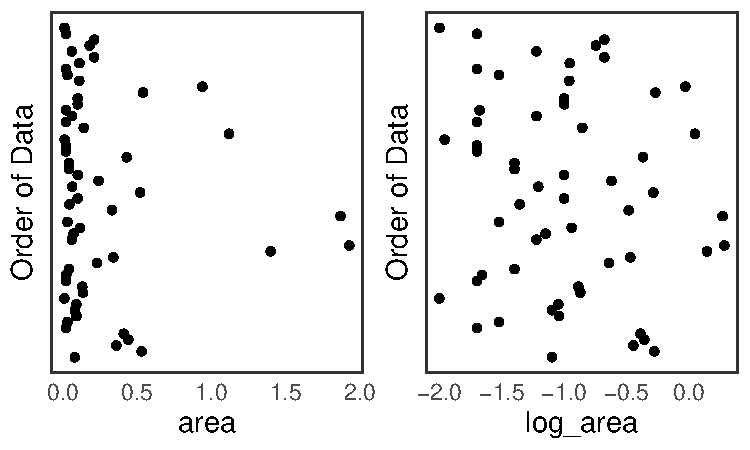
\includegraphics{Bayesian_GLMs_files/figure-latex/ch5-logarea-1} 

}

\caption{\textbf{Dotplots of loch surface area (area) and log10 surface area (log\_area) on North Uist. Data are arranged by the order they appear in the dataframe.}}\label{fig:ch5-logarea}
\end{figure}

\hypertarget{pois-dist}{%
\subsubsection{Distribution of the dependent variable}\label{pois-dist}}

The distribution of the dependent variable will inform selection of the appropriate statistical model to use. Here we visualise stickleback lateral plate number by dividing the x-axis into `bins' and counting the number of observations in each bin as a frequency polygon using the \texttt{geom\_freqpoly()} function from the \texttt{ggplot2} package:

\texttt{ga\ \%\textgreater{}\%\ ggplot(aes(plate))\ +\ geom\_freqpoly(\ bins\ =\ 9)\ +\ labs(x\ =\ "Number\ of\ lateral\ plates",\ y\ =\ "Frequency")\ +\ theme\_classic()\ +\ \ theme(panel.border\ =\ element\_rect(colour\ =\ "black",\ fill=NA,\ size\ =\ 1))}



\begin{figure}

{\centering 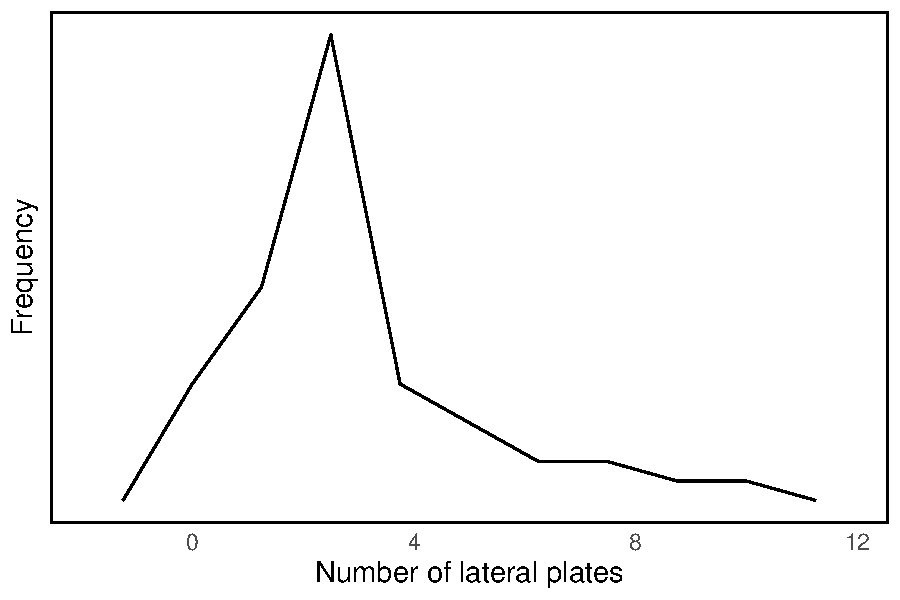
\includegraphics{Bayesian_GLMs_files/figure-latex/ch5-freqpoly-1} 

}

\caption{\textbf{Frequency polygon of mean lateral plate number of three-spined sticklebacks from 57 North Uist lochs.}}\label{fig:ch5-freqpoly}
\end{figure}

The frequency polygon plot of the dependent variable (Fig. \ref{fig:ch5-freqpoly}) shows a distribution with a pronounced positive skew.

\hypertarget{pois-balance}{%
\subsubsection{Balance of categorical variables}\label{pois-balance}}

The balance of the three categorical ecological variables; \texttt{comp} (the presence in a loch of nine-spined sticklebacks, which are competitors of three-spined sticklebacks), \texttt{inve} (the presence of invertebrate predators), and \texttt{vert} (the presence of vertebrate predators), can be checked using the \texttt{table} function

Competitors present in loch?

\texttt{table(ga\$comp)}

\begin{verbatim}
 no yes 
 33  24 
\end{verbatim}

Invertebrate predators present in loch?

\texttt{table(ga\$inve)}

\begin{verbatim}
 no yes 
 32  25 
\end{verbatim}

Vertebrate predators present in loch?

\texttt{table(ga\$vert)}

\begin{verbatim}
 no yes 
  8  49 
\end{verbatim}

Balance is not perfect, though for \texttt{comp} and \texttt{inve} it is acceptable. For \texttt{vert} it is more problematic should we attempt to include this variable in a complex model with multiple other variables, and especially as an interaction.

\hypertarget{pois-collin}{%
\subsubsection{Multicollinearity among covariates}\label{pois-collin}}

If covariates in a model are correlated, then the model may produce unstable parameter estimates with inflated standard errors and it is important to carefully check relationships among covariates.

A comprehensive summary of the relationships among model covariates can be obtained using the \texttt{ggpairs} function from the \texttt{GGally} library:



\texttt{ga\ \%\textgreater{}\%\ ggpairs(columns\ =\ c("dist",\ "alt",\ "log\_area",\ "ph",\ "comp",\ "inve",\ "vert",\ "sl"),\ aes(alpha\ =\ 0.8),\ lower\ =\ list(continuous\ =\ "smooth\_loess"))}

\begin{figure}

{\centering 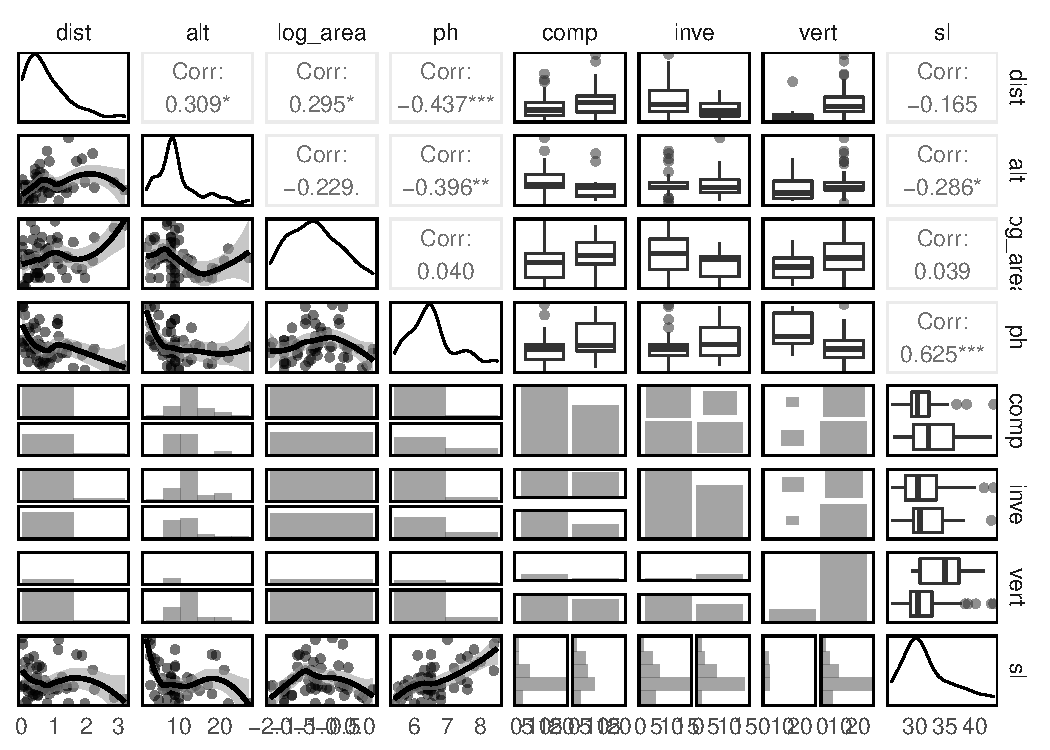
\includegraphics{Bayesian_GLMs_files/figure-latex/ch5-ggpairs-1} 

}

\caption{\textbf{Plot matrix of covariates showing frequency plots, boxplots, frequency histograms, scatterplots, frequency polygons, and pairwise correlations.}}\label{fig:ch5-ggpairs}
\end{figure}

The plot matrix in Fig. \ref{fig:ch5-ggpairs} demonstrates collinearity between loch pH (\texttt{ph}) and mean fish standard length (\texttt{sl}). Since these variables will appear together in model M09 (Table 5.1) we need to explore this relationship further.

The variance inflation factor (VIF) provides an estimate of the proportion of variance in one predictor explained by the other predictors in a model. A VIF of 1 indicates no collinearity. VIF values above 1 indicate increasing degrees of collinearity. VIF values exceeding 3 are considered problematic (Zuur et al.~2010). The VIF can be estimated using the \texttt{vif} function from the \texttt{car} package:

\texttt{round(vif(glm(plate\ \textasciitilde{}\ ph\ +\ sl,\ family\ =\ "poisson",\ data\ =\ ga)),2)}

\begin{verbatim}
  ph   sl 
1.95 1.95 
\end{verbatim}

The estimates of VIF are \textless3, so there is no serious problem with multicollinearity with these two variables.

\hypertarget{pois-zeros}{%
\subsubsection{Zeros in the response variable}\label{pois-zeros}}

The number of zeros in the response variable needs to be considered and will inform selection of the appropriate statistical model. The proportion of zeros in the response variable can be calculated with:

\texttt{round((sum(ga\$plate\ ==\ 0)\ /\ nrow(ga))*100,0)}

11

The response variable comprises 11\% zeros. This proportion of zeros is not necessarily a problem, but is a consideration in deciding how to model the data.

\hypertarget{pois-rels}{%
\subsubsection{Relationships among dependent and independent variables}\label{pois-rels}}

Visual inspection of the data using plots is a critical step and will illustrate whether relationships are linear or non-linear and whether there are interactions between covariates. Start by plotting plate number (the response variable) against the continuous covariates, R code is available in the R script associated with this chapter:



\begin{figure}

{\centering 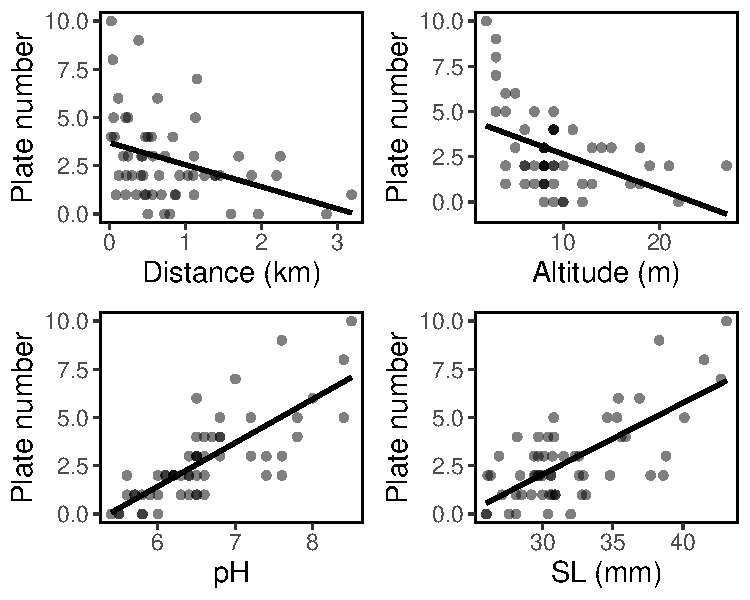
\includegraphics{Bayesian_GLMs_files/figure-latex/ch5-scatter-1} 

}

\caption{\textbf{Multipanel scatterplots of median three-spined stickleback lateral plate number against continuous covariates.}}\label{fig:ch5-scatter}
\end{figure}

The plots shown in Fig. \ref{fig:ch5-scatter} suggest positive (\texttt{pH}, \texttt{SL}) and negative (\texttt{dist}, \texttt{alt}) relationships with plate number. This is not surprising, given that we are using an IT approach and fitting a series of models with variables previously proposed as predicting plate number (Table 5.1). The question we are addressing in this study is not whether these relationships exist, but instead which model (i.e.~hypothesis) is best supported by the data.

For categorical covariates the pattern is less pronounced (the code for this plot is available in the R script associated with this chapter):



\begin{figure}

{\centering 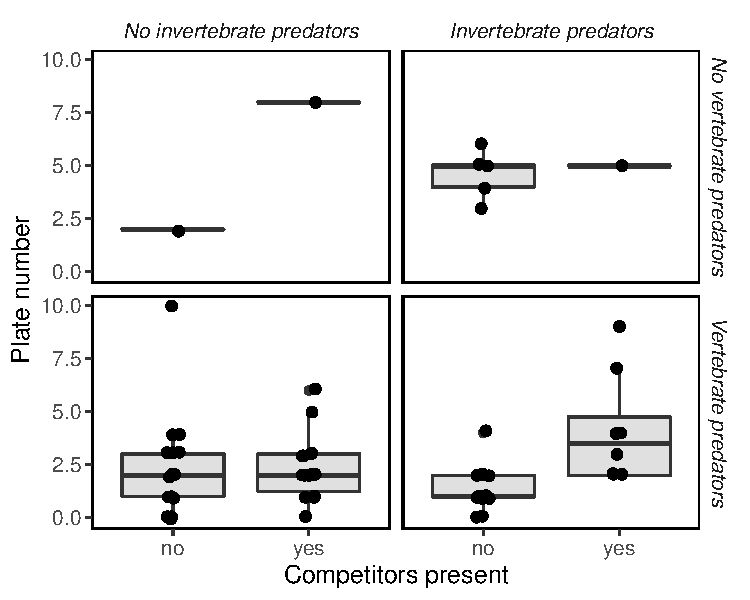
\includegraphics{Bayesian_GLMs_files/figure-latex/ch5-cat-vars-1} 

}

\caption{\textbf{Boxplots of median three-spined stickleback lateral plate number as a function of the presence/absence of a competitor species, invertebrate predators and vertebrate predators.}}\label{fig:ch5-cat-vars}
\end{figure}

The plots shown in Fig. \ref{fig:ch5-cat-vars} suggest variation in lateral plate number as a function of the presence of predators and competitors. Again, however, in the context of an IT approach, these patterns are expected and the question is which \emph{a priori} models are best supported by the data.

\hypertarget{pois-indep}{%
\subsubsection{Independence of response variable}\label{pois-indep}}

An assumption of a GLM is that each observation in a dataset is independent of all others. In the case of the present study each row of data represents a discrete freshwater loch supporting a different three-spined stickleback population. Ostensibly then, these data are independent. However, there is the potential for spatial dependency in these data. North Uist shows striking environmental spatial heterogeneity with the West coast of the island characterised by a band of calcium-rich shell-sand grassland, termed the \emph{machair}, while in the central and eastern regions the \emph{machair} gives way to blanket peat bogs with acidic lochs. A GLM does not permit spatial (or temporal) dependency to be adequately modelled and so, for the purposes of this analysis, while we will treat the data as independent, though this may not strictly be the case.

\hypertarget{pois-select}{%
\subsection{Selection of a statistical model}\label{pois-select}}

The study was designed to compare alternative hypotheses for the evolution of lateral plate number in three-spined sticklebacks. The dependent variable comprises lateral plate counts that include zero, though negative values are not possible. The distribution of the response variable is positively skewed (Fig. \ref{fig:ch5-freqpoly}). The data will be treated as independent, though given the structure of the environment on North Uist, there may be spatial dependency in the data.

Given these conditions, a Poisson is an appropriate distribution as a starting point to model the data, in combination with a log link function. The Poisson is a non-normal distribution that is effective for modelling strictly positive integer data (such as counts). It has a single parameter (lambda, \(\lambda\)), which is both the mean and variance of the response variable. Sometimes you might see mu (\(\mu\)) used to represent the mean. The variance in the Poisson distribution is proportional to the mean so that larger mean values have larger variation. In the context of an INLA model, a Poisson model has no hyperparameter.

The link function is used to link the response variable (counts of lateral plates) and the predictor function (covariates). In the case of a Poisson GLM the default is a log link function. The link function is needed to ensure model fitted values remain positive, while allowing zeros in the data.

\hypertarget{pois-prior-spec}{%
\subsection{Specification of priors}\label{pois-prior-spec}}

An important decision for any Bayesian model is to resolve what priors to place on model parameters. Here we obtain informative priors using published data on three-spined stickleback lateral plate number from across the entire European range of the species.

\hypertarget{existing-data}{%
\subsubsection{Existing data}\label{existing-data}}

Data came from a large-scale study to investigate the morphological variability of three-spined sticklebacks in Europe, with samples collected from 85 locations in England, Estonia, France, Norway, Poland, Turkey and Scotland including samples from North Uist. Results of the study were published in \citet{Smith_2020}.

\hypertarget{pois-priors-fixed}{%
\subsubsection{Priors on the fixed effects}\label{pois-priors-fixed}}

Priors were obtained by fitting the nine models in Table 5.1 using frequentist Poisson GLMs to the data from Smith et al.~(2020) (analysis not shown).

Non-informative (default) priors for all models were \emph{N}(mean = 0, \(\sigma^2\) = 0) (\(\tau\) = 0) on model intercepts (\(\beta1\)) and N(0, 1000) (\(\tau\) = 0. 001) on all other model parameters (\(\beta2\) and \(\beta3\)).

Informative priors for parameters for each model are summarised in Table 5.2.

Table 5.2: \textbf{Informative priors on fixed effects of \emph{a priori} models for the evolution of lateral plates of three-spined sticklebacks on North Uist, showing model number, formulation, and mean, variance and precision for betas.}

\begin{longtable}[]{@{}llccc@{}}
\toprule
Model & Formulation & \(\beta1\) & \(\beta2\) & \(\beta3\) \\
\midrule
\endhead
M01 & vert & \emph{N}(2.1,0.25) & \emph{N}(1.4,0.36) & - \\
& & (\(\tau\) = 4.0) & (\(\tau\) = 2.8) & - \\
M02 & ph & \emph{N}(-3.3,0.64) & \emph{N}(0.7,0.04) & - \\
& & (\(\tau\) = 1.6) & (\(\tau\) = 25) & - \\
M03 & inve & \emph{N}(1.1,0.09) & \emph{N}(0.4,0.09) & - \\
& & (\(\tau\) = 11.1) & (\(\tau\) = 11.1) & - \\
M04 & alt + dist & \emph{N}(2.5,0.09) & \emph{N}(-0.01,0.01) & \emph{N}(-0.1,0.01) \\
& & (\(\tau\) = 11.1) & (\(\tau\) = 100) & (\(\tau\) = 100) \\
M05 & alt + area & \emph{N}(2.9,0.49) & \emph{N}(-0.01,0.01) & \emph{N}(-0.02,0.01) \\
& & (\(\tau\) = 2.0) & (\(\tau\) = 100) & (\(\tau\) = 100) \\
M06 & comp & \emph{N}(1.6,0.09) & \emph{N}(0.5,0.09) & - \\
& & (\(\tau\) = 11.1) & (\(\tau\) = 11.1) & - \\
M07 & vert + ph & \emph{N}(-4.8,3.61) & \emph{N}(0.6,0.25) & \emph{N}(0.6,0.04) \\
& & (\(\tau\) = 0.3) & (\(\tau\) = 4.0) & (\(\tau\) = 25) \\
M08 & vert + comp & \emph{N}(1.7,0.16) & \emph{N}(0.7,0.09) & \emph{N}(0.9,0.09) \\
& & (\(\tau\) = 6.3) & (\(\tau\) = 11.1) & (\(\tau\) = 11.1) \\
M09 & ph + sl & \emph{N}(-3.4,0.36) & \emph{N}(0.5,0.04) & \emph{N}(0.1,0.0025) \\
& & (\(\tau\) = 2.8) & (\(\tau\) = 25.0) & (\(\tau\) = 400) \\
\bottomrule
\end{longtable}

\hypertarget{pois-fit-models}{%
\subsection{Fit the models}\label{pois-fit-models}}

We will fit Bayesian Poisson GLMs using INLA to all the \emph{a priori} models in Table 5.1, first with default priors (\texttt{M01-M09}), and second with informative priors on the fixed effects (\texttt{I01-I09}).

We start by specifying the model formulae:

\texttt{f01\ \textless{}-\ plate\ \textasciitilde{}\ vert}

\texttt{f02\ \textless{}-\ plate\ \textasciitilde{}\ ph}

\texttt{f03\ \textless{}-\ plate\ \textasciitilde{}\ inve}

\texttt{f04\ \textless{}-\ plate\ \textasciitilde{}\ alt\ +\ dist}

\texttt{f05\ \textless{}-\ plate\ \textasciitilde{}\ alt\ +\ log\_area}

\texttt{f06\ \textless{}-\ plate\ \textasciitilde{}\ comp}

\texttt{f07\ \textless{}-\ plate\ \textasciitilde{}\ vert\ +\ ph}

\texttt{f08\ \textless{}-\ plate\ \textasciitilde{}\ vert\ +\ comp}

\texttt{f09\ \textless{}-\ plate\ \textasciitilde{}\ ph\ +\ sl}

Then run the default models \texttt{M01-M09}, specifying \texttt{control.compute\ =\ list(dic\ =\ TRUE)} to enable model comparison:

\texttt{M01\ \textless{}-\ inla(f01,\ control.compute\ =\ list(dic\ =\ TRUE),\ family\ =\ "poisson",\ data\ =\ ga)}

\texttt{M02\ \textless{}-\ inla(f02,\ control.compute\ =\ list(dic\ =\ TRUE),\ family\ =\ "poisson",\ data\ =\ ga)}

\texttt{M03\ \textless{}-\ inla(f03,\ control.compute\ =\ list(dic\ =\ TRUE),\ family\ =\ "poisson",\ data\ =\ ga)}

\texttt{M04\ \textless{}-\ inla(f04,\ control.compute\ =\ list(dic\ =\ TRUE),\ family\ =\ "poisson",\ data\ =\ ga)}

\texttt{M05\ \textless{}-\ inla(f05,\ control.compute\ =\ list(dic\ =\ TRUE),\ family\ =\ "poisson",\ data\ =\ ga)}

\texttt{M06\ \textless{}-\ inla(f06,\ control.compute\ =\ list(dic\ =\ TRUE),\ family\ =\ "poisson",\ data\ =\ ga)}

\texttt{M07\ \textless{}-\ inla(f07,\ control.compute\ =\ list(dic\ =\ TRUE),\ family\ =\ "poisson",\ data\ =\ ga)}

\texttt{M08\ \textless{}-\ inla(f08,\ control.compute\ =\ list(dic\ =\ TRUE),\ family\ =\ "poisson",\ data\ =\ ga)}

\texttt{M09\ \textless{}-\ inla(f09,\ control.compute\ =\ list(dic\ =\ TRUE),\ family\ =\ "poisson",\ data\ =\ ga)}

We can compare model fit in a Bayesian framework using the Deviance Information Criterion (DIC). Like AIC, a smaller DIC score indicates a better fit of the model to the data given its complexity.

First extract the default DICs:

\texttt{DefDIC\ \textless{}-\ c(M01\$dic\$dic,M02\$dic\$dic,M03\$dic\$dic,M04\$dic\$dic,\ M05\$dic\$dic,M06\$dic\$dic,M07\$dic\$dic,\ M08\$dic\$dic,M09\$dic\$dic)}

Add weighting and names to the DIC scores and tabulate the model DICs based on order of fit:

\texttt{DefDIC.weights\ \textless{}-\ aicw(DefDIC)}

\texttt{DefDIC.weights\ \%\textgreater{}\%\ mutate(model\ =\ c("M01","M02","M03",\ "M04","M05","M06",\ "M07","M08","M09"))\ \%\textgreater{}\%\ select(model,\ everything())\ \%\textgreater{}\%\ arrange(fit)\ \%\textgreater{}\%\ mutate(across(2:4,\ round,\ 2))}

\begin{verbatim}
  model      fit     delta            w
1   M09 190.9668  0.000000 7.870939e-01
2   M02 194.2876  3.320843 1.495942e-01
3   M07 196.0073  5.040565 6.331139e-02
4   M04 219.7739 28.807145 4.371541e-07
5   M05 224.4571 33.490294 4.204376e-08
6   M08 231.9562 40.989422 9.892057e-10
7   M01 236.4772 45.510416 1.031728e-10
8   M06 243.6950 52.728229 2.794070e-12
9   M03 246.5361 55.569332 6.749933e-13
\end{verbatim}

We can summarise this output for presentation:

Table 5.3: \textbf{Non-informative \emph{a priori} models ranked by Deviance Information Criterion (DIC) score. Delta \emph{i} is the difference in DIC scores, omega is DIC weighting.}

\begin{longtable}[]{@{}lccc@{}}
\toprule
Model & DIC & \(\Delta\)\emph{i} & \(\omega\) \\
\midrule
\endhead
M09 & 191.0 & 0.0 & 0.79 \\
M02 & 194.3 & 3.3 & 0.15 \\
M07 & 196.0 & 5.0 & 0.06 \\
M04 & 219.8 & 28.2 & 0.00 \\
M05 & 224.5 & 33.5 & 0.00 \\
M08 & 232.0 & 41.0 & 0.00 \\
M01 & 236.5 & 45.5 & 0.00 \\
M06 & 243.7 & 52.7 & 0.00 \\
M03 & 246.5 & 55.6 & 0.00 \\
\bottomrule
\end{longtable}

Table 5.3 summarises the relative performance of the non-informative \emph{a priori} models, ranked by DIC score. \(\Delta_i\) is the difference in DIC scores between the best fitting and alternative candidate models. Model weight (omega, \(\omega\)) can be interpreted as the probability that a given model is the best model (based on DIC), given the data and the set of alternative models. In this case model \texttt{M09} is by far the most probable. Note that this result does not preclude the possibility that another, untested, \emph{a priori} model could not provide a better fit to the data.

We now run models \texttt{I01-I09} using the informative priors summarised in Table 5.2 (the coding is available in the R script associated with this chapter), which gives us:

\begin{verbatim}
##   model      fit     delta            w
## 1   I09 189.3950  0.000000 8.417945e-01
## 2   I02 193.3424  3.947416 1.169595e-01
## 3   I07 195.4269  6.031980 4.124567e-02
## 4   I04 219.4634 30.068461 2.488414e-07
## 5   I05 223.3790 33.984036 3.512905e-08
## 6   I08 234.2935 44.898568 1.498325e-10
## 7   I01 236.5881 47.193120 4.757189e-11
## 8   I06 243.4523 54.057320 1.537476e-12
## 9   I03 245.9701 56.575135 4.365878e-13
\end{verbatim}

Which we can summarise more neatly:

Table 5.4: \textbf{Informative \emph{a priori} models ranked by Deviance Information Criterion (DIC) score. Delta \emph{i} is the difference in DIC scores, omega is DIC weighting.}

\begin{longtable}[]{@{}lccc@{}}
\toprule
Model & DIC & \(\Delta\)\emph{i} & \(\omega\) \\
\midrule
\endhead
I09 & 189.4 & 0.0 & 0.84 \\
I02 & 193.3 & 3.9 & 0.12 \\
I07 & 195.4 & 6.0 & 0.04 \\
I04 & 219.5 & 30.1 & 0.00 \\
I05 & 223.4 & 34.0 & 0.00 \\
I08 & 234.3 & 44.9 & 0.00 \\
I01 & 236.6 & 47.2 & 0.00 \\
I06 & 243.5 & 54.1 & 0.00 \\
I03 & 246.0 & 56.6 & 0.00 \\
\bottomrule
\end{longtable}

The rank order of informative models (Table 5.3) is identical to that for non-informative models (Table 5.4), though DIC scores and model weights (\(\omega\)) vary somewhat. Model \texttt{I09} is again the most probable given the data and the set of candidate models.

Compare the best-fitting models with non-informative and informative priors:

\texttt{ComDIC\ \textless{}-\ c(M09\$dic\$dic,\ I09\$dic\$dic)}

\texttt{DIC\ \textless{}-\ cbind(ComDIC)}

\texttt{rownames(DIC)\ \textless{}-\ c("default\ priors","informative\ priors")}

\texttt{round(DIC,0)}

\begin{verbatim}
                   ComDIC
default priors        191
informative priors    189
\end{verbatim}

These DIC scores are essentially the same.

\hypertarget{obtain-the-posterior-distribution-1}{%
\subsection{Obtain the posterior distribution}\label{obtain-the-posterior-distribution-1}}

\hypertarget{pois-def-priors}{%
\subsubsection{Model with default priors}\label{pois-def-priors}}

Output for the fixed effects of M09 can be obtained with:

\texttt{M09Betas\ \textless{}-\ M09\$summary.fixed{[},c("mean",\ "sd",\ "0.025quant",\ "0.975quant"){]}}

\texttt{round(M09Betas,\ digits\ =\ 3)}

\begin{verbatim}
              mean    sd 0.025quant 0.975quant
(Intercept) -4.011 0.657     -5.305     -2.724
ph           0.488 0.126      0.242      0.735
sl           0.052 0.022      0.007      0.095
\end{verbatim}

This output reports the posterior mean, standard deviation and 95\% credible intervals for the intercept and covariates (\texttt{ph}, \texttt{sl}).

For the variable \texttt{ph} we have a posterior mean of 0.49 and lower 95\% credible interval of 0.24 and upper 95\% credible interval of 0.74. We can conclude from this result that we are 95\% certain that the posterior mean of the regression parameter for \texttt{ph} falls between these credible intervals; \texttt{ph} is statistically important in the model.

Similarly, we can conclude that for the relationship between stickleback standard length (\texttt{sl}) and lateral plate number the credible intervals range from 0.01 to 0.10, indicating that this model parameter differs from zero.

The model intercept, with credible intervals between -5.31 and -2.72, differs from zero with a posterior mean of -4.01 and standard deviation of 0.66.

The posterior distribution of the fixed effects can be visualized using \texttt{ggplot2.} The coding for this plot is available in the R script associated with this chapter.



\begin{figure}

{\centering 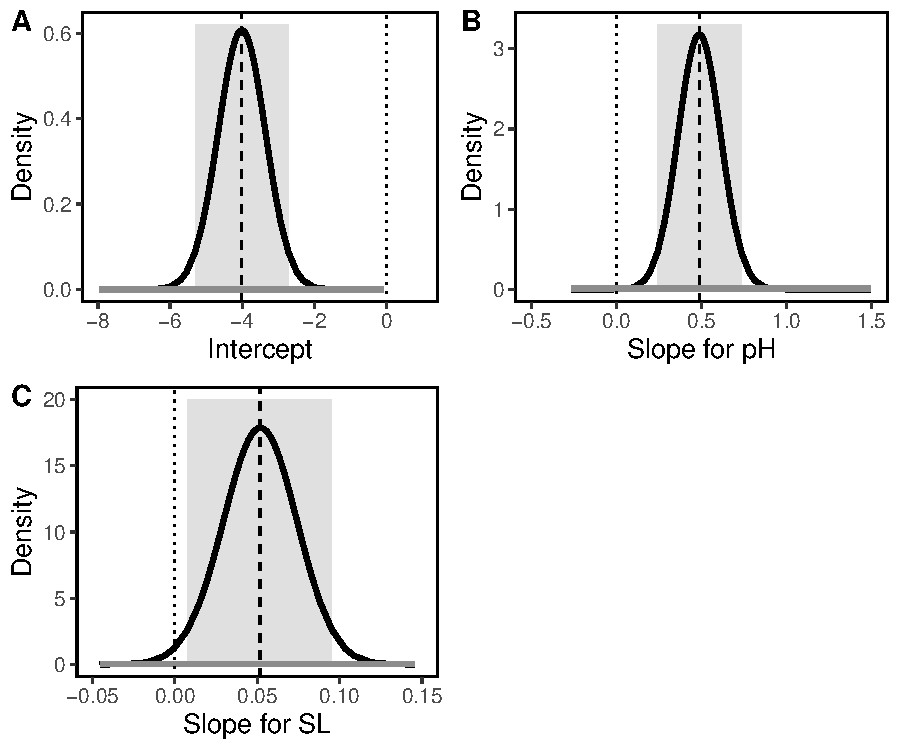
\includegraphics{Bayesian_GLMs_files/figure-latex/ch5-M9-betas-1} 

}

\caption{\textbf{Posterior and prior distributions for fixed parameters of a Bayesian linear regression to model lateral plate number of three-spined sticklebacks (\emph{Gasterosteus aculeatus}) on North Uist. The model is fitted with default (non-informative) priors. Distributions for: A. model intercept; B. slope for pH; C. slope for standard length. The solid black line is the posterior distribution, the solid gray line is the prior distribution, the gray shaded area encompasses the 95\% credible intervals, the vertical dashed line is the posterior mean of the parameter, the vertical dotted line indicates zero. For parameters where zero (indicated by dotted line) falls outside the range of the 95\% credible intervals (gray shaded area), the parameter is considered statistically important.}}\label{fig:ch5-M9-betas}
\end{figure}

Figure \ref{fig:ch5-M9-betas} provides a visual representation of the summary of the fixed effects, and indicates that for model \texttt{M09} the intercept and slope for pH and male standard length differ from zero and are statistically important. This figure also shows the non-informative priors, which appear flat across the range of possible values, thus making a limited contribution to the posterior distribution.

\hypertarget{pois-inf-priors}{%
\subsubsection{Model with informative priors}\label{pois-inf-priors}}

As for the default model, we will examine the posterior distributions for the model with informative priors, starting with the fixed effects.

\hypertarget{fixed-effects-2}{%
\subsubsection{Fixed effects}\label{fixed-effects-2}}

First examine the posterior mean and 95\% credible intervals for the fixed effects:

\texttt{I09Betas\ \textless{}-\ I09\$summary.fixed{[},c("mean",\ "sd",\ "0.025quant",\ "0.975quant"){]}}

\texttt{round(I09Betas,\ digits\ =\ 2)}

\begin{verbatim}
             mean   sd 0.025quant 0.975quant
(Intercept) -3.74 0.43      -4.59      -2.89
ph           0.44 0.10       0.25       0.62
sl           0.05 0.02       0.02       0.09
\end{verbatim}

Note that the qualitative outcome of model I09 is the same as the model with default priors (M09), but in the case of informative priors the posterior means differ quantitatively, as do the 95\% credible intervals which encompass a narrower range in each case.

The posterior distributions of the fixed effects can be visualized using \texttt{ggplot2}. The coding for this plot is available in the R script associated with this chapter.



\begin{figure}

{\centering 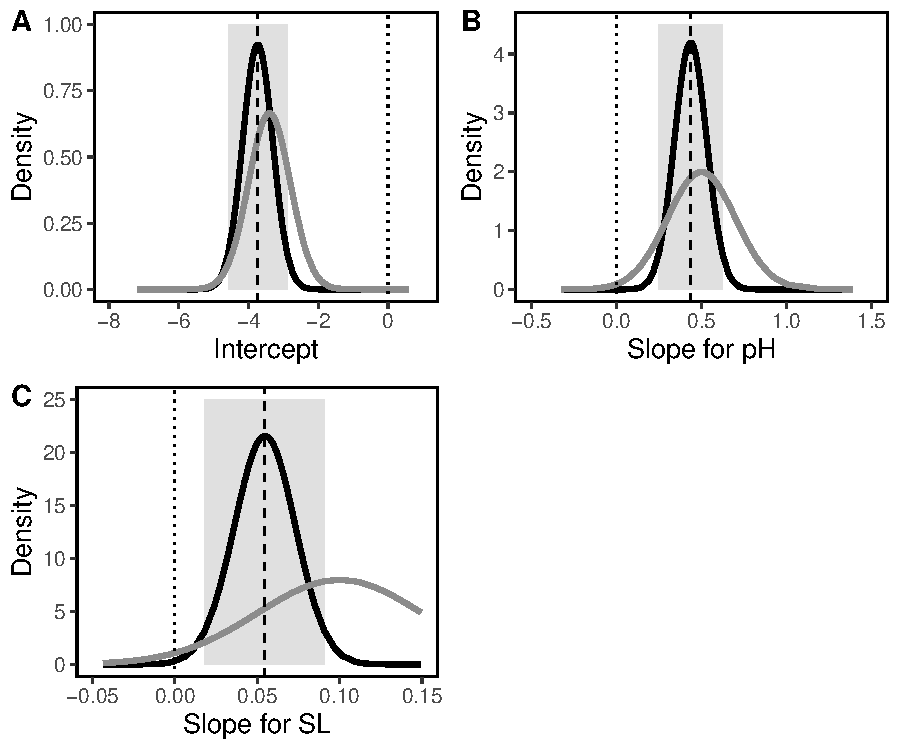
\includegraphics{Bayesian_GLMs_files/figure-latex/ch5-I9-betas-1} 

}

\caption{\textbf{Posterior and prior distributions for fixed parameters of a Bayesian linear regression to model lateral plate number of three-spined sticklebacks (\emph{Gasterosteus aculeatus}) on North Uist. The model is fitted with informative priors. Distributions for: A. model intercept; B. slope for pH; C. slope for standard length. The solid black line is the posterior distribution, the solid gray line is the prior distribution, the gray shaded area encompasses the 95\% credible intervals, the vertical dashed line is the posterior mean of the parameter, the vertical dotted line indicates zero. For parameters where zero (indicated by dotted line) falls outside the range of the 95\% credible intervals (gray shaded area), the parameter is considered statistically important.}}\label{fig:ch5-I9-betas}
\end{figure}

Figure \ref{fig:ch5-I9-betas} indicates that for model I09 the intercept, slope for pH and male standard length all differ from zero and are statistically important. The distributions of the informative priors are based on data from a Europe-wide study of three-spined stickleback morphology (priors summarised in Table 5.2).

\hypertarget{pois-freq-comp}{%
\subsubsection{Comparison with frequentist Poisson GLM}\label{pois-freq-comp}}

We can compare the results of the best-fitting Bayesian Poisson GLMs obtained with non-informative and informative priors (M09 and I09) with the same model fitted in a frequentist setting. Execution of the model in a frequentist framework can be performed with:

\texttt{Freq\ \textless{}-\ glm(plate\ \textasciitilde{}\ ph\ +\ sl,\ family\ =\ "poisson",\ data\ =\ ga)}

The results are obtained with:

\texttt{round(summary(Freq)\$coef{[},1:4{]},3)}

\begin{verbatim}
            Estimate Std. Error z value Pr(>|z|)
(Intercept)   -4.013      0.657  -6.106    0.000
ph             0.488      0.126   3.885    0.000
sl             0.052      0.022   2.316    0.021
\end{verbatim}

We already have the results for the Bayesian models, but these can be displayed for the model with default priors with:

\texttt{round(M09Betas,\ digits\ =\ 3)}

\begin{verbatim}
              mean    sd 0.025quant 0.975quant
(Intercept) -4.011 0.657     -5.305     -2.724
ph           0.488 0.126      0.242      0.735
sl           0.052 0.022      0.007      0.095
\end{verbatim}

And for the best-fitting model with informative priors:

\texttt{round(I09Betas,\ digits\ =\ 3)}

\begin{verbatim}
              mean    sd 0.025quant 0.975quant
(Intercept) -3.737 0.432     -4.585     -2.891
ph           0.436 0.095      0.249      0.623
sl           0.054 0.019      0.018      0.091
\end{verbatim}

Results can be combined and presented formally:

Table 5.5: \textbf{Parameters for fixed effects of a model to investigate the evolution of lateral plate number in three-spined sticklebacks on North Uist for a frequentist GLM, Bayesian GLM with default priors and Bayesian GLM with informative priors. Mean (sd) parameter estimates are shown for each model.}

\begin{longtable}[]{@{}lccc@{}}
\toprule
Model & Intercept & pH & sl \\
\midrule
\endhead
Frequentist & -4.01(0.66) & 0.49(0.13) & 0.05(0.02) \\
Bayesian (default) & -4.01(0.66) & 0.49(0.13) & 0.05(0.02) \\
Bayesian (informative) & -3.74(0.43) & 0.44(0.10) & 0.05(0.02) \\
\bottomrule
\end{longtable}

While parameter estimates for the frequentist and Bayesian model with non-informative priors are almost identical, results for the Bayesian model with informative priors diverge slightly, with parameter estimates having slightly lower variance.

\hypertarget{conduct-model-checks-1}{%
\subsection{Conduct model checks}\label{conduct-model-checks-1}}

After model fitting and obtaining the posterior distributions, the next step is validation of the model through model checks.

\hypertarget{pois-dic}{%
\subsubsection{Model selection using the Deviance Information Criterion (DIC)}\label{pois-dic}}

We adopted an information theoretic (IT) approach in this analysis, fitting nine biologically plausible alternative \emph{a priori} models using both non-informative and informative priors. We assessed model fit using the DIC (Section 5.7) and identified models \texttt{M09} and \texttt{I09} as the most probable.

Given the approach we have used, there is no justification for undergoing further model selection. An exception might be a case in which two or more models are equally probable, in which case we might consider a model averaging procedure to arrive at an optimum model. However, in the case of the present study, there was no ambiguity concerning the best-fitting model.

\hypertarget{pois-disp}{%
\subsubsection{Dispersion}\label{pois-disp}}

Poisson GLMs assume that the mean and variance of the response variable vary at the same rate. This assumption must be confirmed. Overdispersion means that a Poisson distribution does not adequately model the variance and is not appropriate for the analysis.

We will implement the 7-step protocol of \citet{Zuur_2017} to assess dispersion in the Poisson GLM with informative priors:

\begin{enumerate}
\def\labelenumi{\arabic{enumi}.}
\item
  \emph{Apply Poisson GLM in INLA}
\item
  \emph{Simulate a set of regression parameters from the posterior distribution}
\item
  \emph{Calculate expected values}
\item
  \emph{Simulate count data using the \texttt{rpois} function}
\item
  \emph{Calculate Pearson residuals for simulated data}
\item
  \emph{Repeat steps 2-5 x 1000 times}
\item
  \emph{Compare sums of squared Pearson residuals with observed data}
\end{enumerate}

\hypertarget{pois-sim}{%
\paragraph{Apply Poisson GLM in INLA}\label{pois-sim}}

Working just with the model with informative priors for brevity, we re-run the model with the \texttt{config\ =\ TRUE} option to permit the simulation of regression parameters:

\texttt{I09\ \textless{}-\ inla(f09,\ family\ =\ "poisson",\ data\ =\ ga,\ control.\ compute\ =\ list(config\ =\ TRUE),\ control.predictor\ =\ list(\ compute\ =\ TRUE),\ control.fixed\ =\ list(mean.intercept\ =\ -3.4,\ prec.intercept\ =\ 0.6\^{}(-2),\ mean\ =\ list(ph\ =\ 0.5,\ sl\ =\ 0.1),\ prec\ =\ list(ph\ =\ 0.2\^{}(-2),\ sl\ =\ 0.05\^{}(-2))))}

\hypertarget{simulate-regression-parameters-from-the-posterior-distribution}{%
\paragraph{Simulate regression parameters from the posterior distribution}\label{simulate-regression-parameters-from-the-posterior-distribution}}

We use the \texttt{inla.posterior.sample} function to simulate regression parameters with the output stored in the \texttt{SimData} object.

\texttt{set.seed(1966)}

\texttt{SimData\ \textless{}-\ inla.posterior.sample(n\ =\ 1,\ result\ =\ I09)}

SimData comprises 60 rows, with the first 57 rows simulated values and the last 3 rows simulated regression parameters. It can be viewed with:

\texttt{SimData{[}{[}1{]}{]}\$latent}

Note that \texttt{SimData} is just one set of simulated values (we specified n = 1).

\hypertarget{calculate-predicted-values}{%
\paragraph{Calculate predicted values}\label{calculate-predicted-values}}

Start by accessing the last 3 rows of \texttt{SimData} containing the betas and use them to calculate the fitted values:

\texttt{BetaRows\ \textless{}-\ (nrow(SimData{[}{[}1{]}{]}\$latent)\ -\ 2):}

\texttt{nrow(SimData{[}{[}1{]}{]}\$latent)}

\texttt{Betas\ \textless{}-\ SimData{[}{[}1{]}{]}\$latent{[}BetaRows{]}}

\texttt{X\ \textless{}-\ model.matrix(\textasciitilde{}\ ph\ +\ sl,\ data\ =\ ga)}

\texttt{mu\ \textless{}-\ exp(X\ \%*\%\ Betas)}

\hypertarget{simulate-count-data-using-rpois}{%
\paragraph{\texorpdfstring{Simulate count data using \texttt{rpois}}{Simulate count data using rpois}}\label{simulate-count-data-using-rpois}}

Using the \texttt{rpois} function we can simulate a set of 57 plate counts that fit a Poisson distribution:

\texttt{Ysim\ \textless{}-\ rpois(n\ =\ nrow(ga),\ lambda\ =\ mu)}

\hypertarget{calculate-summary-statistic}{%
\paragraph{Calculate summary statistic}\label{calculate-summary-statistic}}

The Pearson residuals for the single set of simulated data can be calculated with:

\texttt{mu1\ \textless{}-\ I09\$summary.fitted.values{[},"mean"{]}}

\texttt{Es\ \textless{}-\ (Ysim\ -\ mu1)\ /sqrt(mu1)}

\texttt{N\ \ \ \ \textless{}-\ nrow(ga)}

\texttt{Npar\ \textless{}-\ length(BetaRows)}

\texttt{round(sum(Es\^{}2)\ /\ (N\ -\ Npar),1)}

The residuals should be close to 1, which is the case.

\hypertarget{repeat-simulation}{%
\paragraph{Repeat simulation}\label{repeat-simulation}}

We now repeat steps 2-5 to generate 1000 simulations:

\texttt{SimData\ \textless{}-\ inla.posterior.sample(n\ =\ 1000,\ result\ =\ I09)}

\texttt{N\ \ \ \ \ \ \textless{}-\ nrow(ga)}

\texttt{Ysim\ \ \ \textless{}-\ matrix(nrow\ =\ N,\ ncol\ =\ 1000)}

\texttt{mu.sim\ \textless{}-\ matrix(nrow\ =\ N,\ ncol\ =\ 1000)\ for\ (i\ in\ 1:1000)\{\ Betas\ \textless{}-\ SimData{[}{[}i{]}{]}\$latent{[}BetaRows{]}\ mu.sim{[},i{]}\ \textless{}-\ exp(X\ \%*\%\ Betas)\ Ysim{[},i{]}\ \ \ \textless{}-\ rpois(n\ =\ N,\ lambda\ =\ exp(X\ \%*\%\ Betas))\}}

This gives us 1000 simulated predictions of plate number.

\hypertarget{compare-dispersion-of-simulated-and-observed-data}{%
\paragraph{Compare dispersion of simulated and observed data}\label{compare-dispersion-of-simulated-and-observed-data}}

Obtain the squared Pearson residuals for the observed data:

\texttt{E1\ \ \textless{}-\ (ga\$plate\ -\ mu1)\ /sqrt(mu1)}

\texttt{Dispersion\ \textless{}-\ sum(E1\^{}2)\ /\ (N\ -\ Npar)}

And the same for the simulated datasets:

\texttt{Dispersion.sim\ \textless{}-\ NULL\ for(i\ in\ 1:1000)\{\ e2\ \textless{}-\ (Ysim{[},i{]}\ -\ mu.sim{[},i{]})\ /sqrt(mu.sim{[},i{]})\ Dispersion.sim{[}i{]}\ \textless{}-\ sum(e2\^{}2)\ /\ (N\ -\ Npar)\ \}}

Plot a frequency histogram of estimates of dispersion for the simulated data:

\texttt{par(mfrow\ =\ c(1,1),\ mar\ =\ c(5,5,2,2),\ cex.lab\ =\ 1.3)\ hist(Dispersion.sim,\ xlab\ =\ "Model\ dispersion",\ ylab\ =\ "Frequency",\ main\ =\ "",\ xlim\ =\ c(0,\ 2.5),\ breaks\ =\ 16)}

And add a black dot to show dispersion for the observed data:

\texttt{points(x\ =\ Dispersion,\ y\ =\ 0,\ pch\ =\ 19,\ cex\ =\ 2.5,\ col\ =\ 1)}



\begin{figure}

{\centering 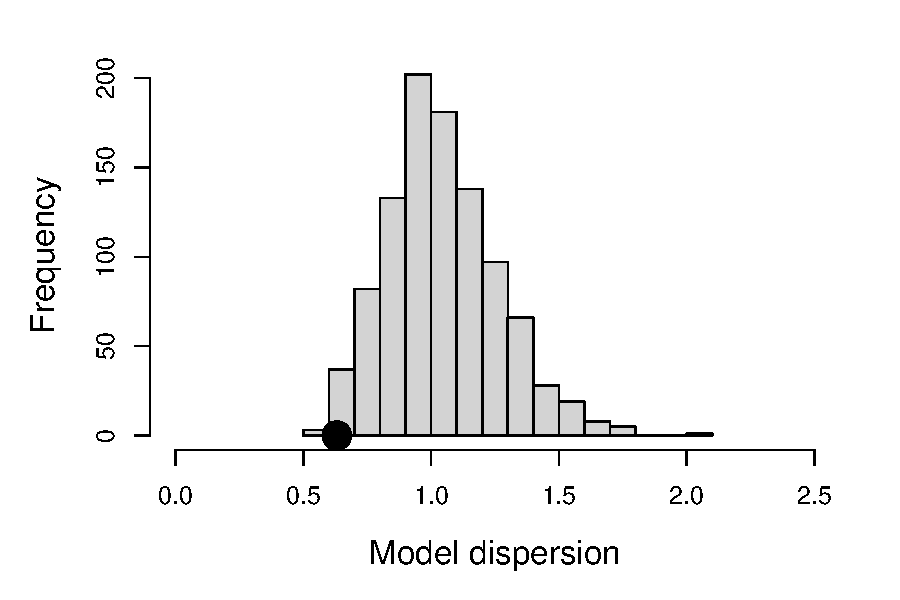
\includegraphics{Bayesian_GLMs_files/figure-latex/ch5-disp-plot-1} 

}

\caption{\textbf{Frequency histogram for 1000 simulated (gray bars) and observed (black dot) dispersion statistics for three-spined stickleback lateral plate counts.}}\label{fig:ch5-disp-plot}
\end{figure}

The dispersion statistic for the observed data (black dot) in Fig. \ref{fig:ch5-disp-plot} is at the lower end of the simulated data sets, indicating mild under-dispersion. Given that data were obtained for strictly freshwater three-spined stickleback populations on North Uist, and lateral plate counts in freshwater populations typically do not exceed 7 lateral plates, mild under-dispersion in the data is not unexpected. Since the observed dispersion falls within the range generated by random simulations (albeit at the lower end), we can conclude that model dispersion is acceptable, though mildly underdispersed, and proceed with model checks.

\hypertarget{pois-ppc}{%
\subsubsection{Posterior predictive checks}\label{pois-ppc}}

Posterior predictive checks are used to assess whether a model generates realistic predictions by drawing simulated estimates from the joint posterior predictive distribution and comparing them with observed data with a posterior predictive p-value. If the posterior predictive p-value is close to 0.5 it means simulated and observed data are similar, whereas if close to 1 it means the model prediction is too high and if close to zero, too low.

See the R script associated with this chapter for estimating and plotting the posterior predictive p-values for the Bayesian model with informative priors without interaction.



\begin{figure}

{\centering 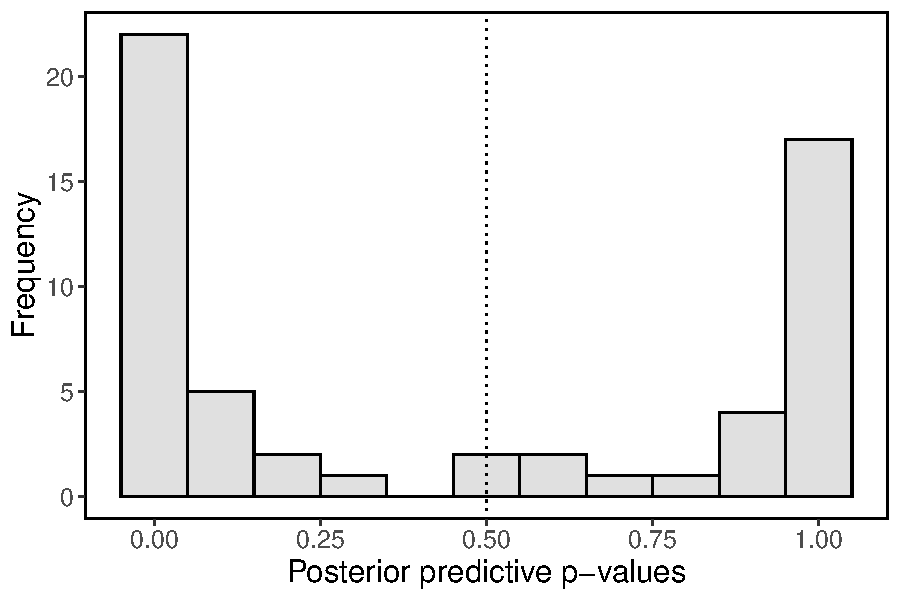
\includegraphics{Bayesian_GLMs_files/figure-latex/ch5-PPC-1} 

}

\caption{\textbf{Frequency histogram of the posterior predictive p-values for the best-fitting Bayesian linear regression with informative priors to predict lateral plate number in three-spined sticklebacks from North Uist. The vertical dotted line indicates 0.5.}}\label{fig:ch5-PPC}
\end{figure}

The frequency histogram of posterior predictive p-values in Fig. \ref{fig:ch5-PPC} shows that most values are close to zero or 1, with few close to 0.5, indicating the model check has not been satisfied; the data are under and over dispersed compared to the model. We will proceed with further model checks.

\hypertarget{pois-cv}{%
\subsubsection{Cross-validation model checking}\label{pois-cv}}

We use leave-one-out cross validation (LOO-CV) to examine how well the model is able to generalise to new data using the conditional predictive ordinate (CPO) and probability integral transform (PIT) to evaluate model goodness-of-fit. To obtain both we simply run the model using the \texttt{cpo\ =\ TRUE} option in \texttt{control.compute}.

To ensure there are no potential numerical problems in estimating CPO or PIT for a given model, we run the following check:

\texttt{sum(I09.pred\$cpo\$failure)}

An outcome of zero indicates no problems with the computation of CPO or PIT.

A uniform distribution of PIT values indicates whether the predictive distributions match the data (see the R script associated with this chapter).



\begin{figure}

{\centering 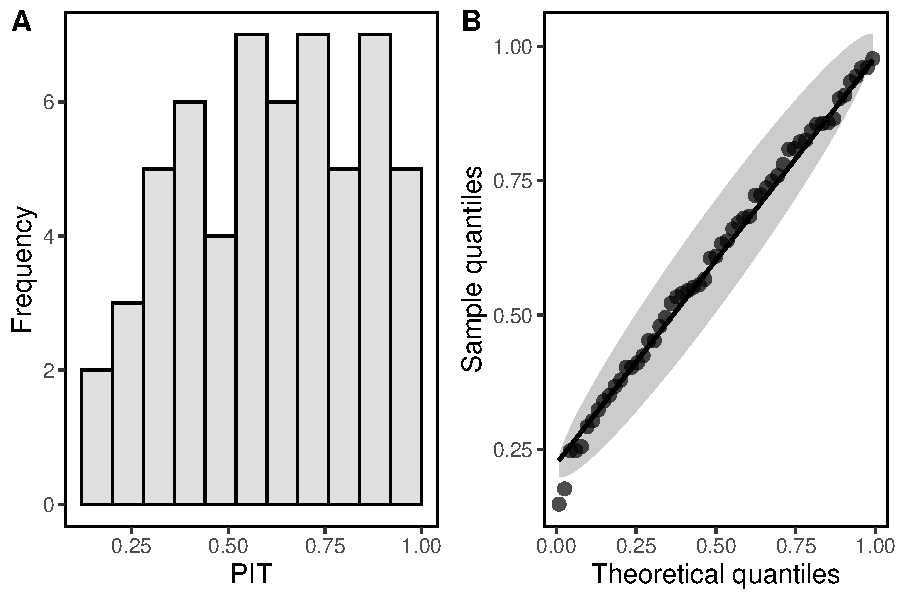
\includegraphics{Bayesian_GLMs_files/figure-latex/ch5-PIT-1} 

}

\caption{\textbf{A. Frequency histogram; B. Uniform Q-Q plot with confidence bands (shaded gray), for cross-validated PIT values for the best-fitting Bayesian Poisson GLM with informative priors.}}\label{fig:ch5-PIT}
\end{figure}

The frequency histogram of PIT values in Fig. \ref{fig:ch5-PIT}A shows that the distribution is broadly uniform. This conclusion is supported by the Q-Q plot (Fig. \ref{fig:ch5-PIT}B), which shows that the PIT values match a uniform distribution.

\hypertarget{pois-resids}{%
\subsubsection{Bayesian residuals analysis}\label{pois-resids}}

Homogeneity of residual variance can be assessed visually by plotting model residual variance against fitted values as well as each variable in the model (see the R script associated with this chapter).



\begin{figure}

{\centering 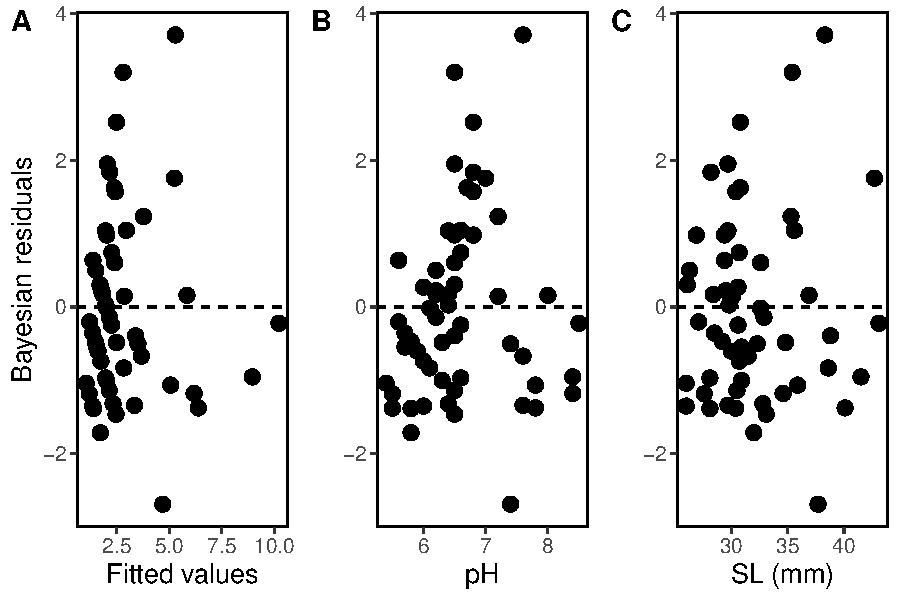
\includegraphics{Bayesian_GLMs_files/figure-latex/ch5-resids-1} 

}

\caption{\textbf{Bayesian residuals plotted against: A. fitted values; B. loch pH; and C. population mean standard length (mm), to assess homogeneity of residual variance.}}\label{fig:ch5-resids}
\end{figure}

Ideally, the distribution of residuals around zero should be random along the horizontal axis. For Fig. \ref{fig:ch5-resids}A there is some deviation from this pattern, though there are few fitted values \textgreater8. For Figs. \ref{fig:ch5-resids}B,C the pattern of residuals is acceptable.

\hypertarget{pois-sens}{%
\subsubsection{Prior sensitivity analysis}\label{pois-sens}}

A final model check is to examine prior distributions through a sensitivity analysis that involves systematically changing prior distributions and examining the magnitude of outcome for the posterior distribution.

We will investigate prior sensitivity by increasing and decreasing priors on the fixed effects by 20\% and examined the outcome for the posterior mean (see the R script associated with this chapter).

The original priors for the fixed effects on model \texttt{I09} were (mean, \(\sigma^2\)):

\(\beta intercept\) \textasciitilde{} \emph{N}(-3.40, 0.36) (\(\tau\) = 2.8)

\(\beta ph\) \textasciitilde{} \emph{N}(0.50, 0.04) (\(\tau\) = 25)

\(\beta sl\) \textasciitilde{} \emph{N}(0.10, 0.0025) (\(\tau\) = 400)

In the case of an increase by 20\%, the priors for the fixed effects are:

\(\beta intercept\) \textasciitilde{} \emph{N}(-2.72, 0.44) (\(\tau\) = 2.3)

\(\beta ph\) \textasciitilde{} \emph{N}(0.60, 0.048) (\(\tau\) = 20.7)

\(\beta sl\) \textasciitilde{} \emph{N}(0.12,0.003) (\(\tau\) = 331)

In the case of a decrease by 20\%, the priors for the fixed effects are:

\(\beta intercept\) \textasciitilde{} \emph{N}(-4.08, 0.29) (\(\tau\) = 3.4)

\(\beta ph\) \textasciitilde{} \emph{N}(0.40, 0.04) (\(\tau\) = 31.2)

\(\beta sl\) \textasciitilde{} \emph{N}(0.08, 0.002) (\(\tau\) = 493.8)

Table 5.6: \textbf{Sensitivity analysis for a 20\% increase and decrease in priors on fixed effects and the \% change in the posterior mean.}

\begin{longtable}[]{@{}lccccc@{}}
\toprule
Parameter & \% prior & Mean & 0.025CI & 0.975CI & \% posterior \\
\midrule
\endhead
& +20 & -3.49 & -4.38 & -2.60 & +6.7 \\
Intercept & 0 & -3.74 & -4.59 & -2.89 & 0 \\
& -20 & -4.04 & -4.83 & -3.24 & -8.0 \\
& & & & & \\
& +20 & 0.42 & 0.23 & 0.62 & -4.5 \\
sl & 0 & 0.44 & 0.25 & 0.62 & 0 \\
& -20 & 0.45 & 0.27 & 0.63 & +2.3 \\
& & & & & \\
& +20 & 0.05 & 0.013 & 0.087 & 0 \\
pH & 0 & 0.05 & 0.018 & 0.091 & 0 \\
& -20 & 0.06 & 0.025 & 0.095 & +11 \\
\bottomrule
\end{longtable}

The results of the prior sensitivity analysis (Table 5.6) show that increases and decreases to priors as large as 20\% result in relatively modest changes to the posterior distribution.

We can additionally plot the posterior distributions of these alternative models (see the R script associated with this chapter).



\begin{figure}

{\centering 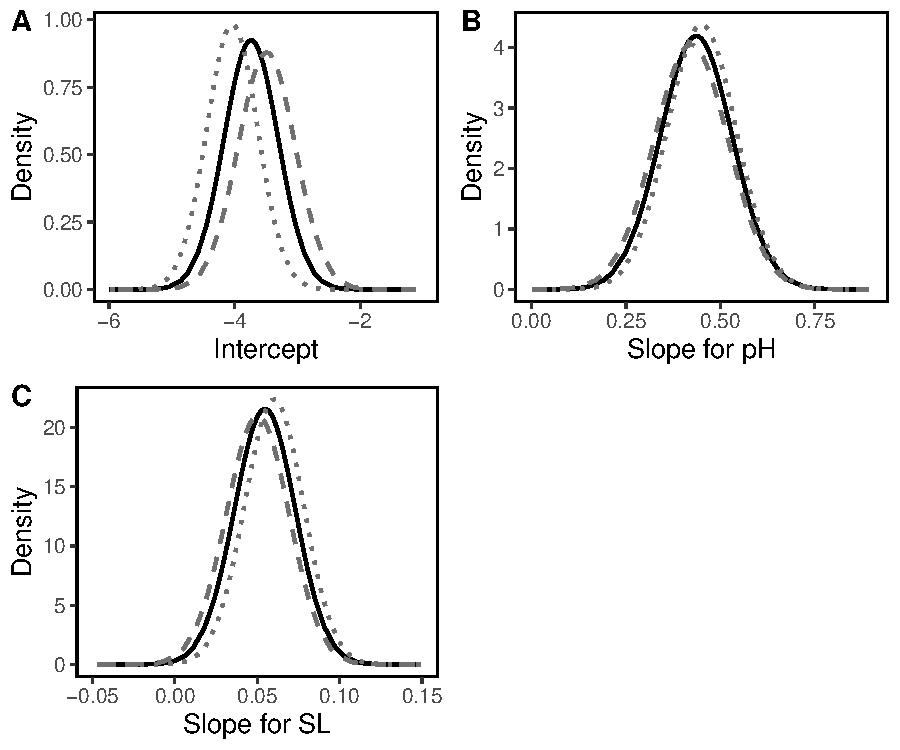
\includegraphics{Bayesian_GLMs_files/figure-latex/ch5-post-plot-1} 

}

\caption{\textbf{Posterior distributions for parameters of a Bayesian Poisson GLM to predict lateral plate number in three-spined sticklebacks from North Uist. Distributions for: A. model intercept; B. slope for pH; C. standard length. The solid black line is the posterior distribution for the optimal model, the dashed gray line is the posterior distribution for an alternative model with the priors increased by 20\%, the dotted gray line is the posterior distribution for an alternative model with the priors decreased by 20\%.}}\label{fig:ch5-post-plot}
\end{figure}

Plots of the posterior distributions for the model fixed effects indicate that the posterior distributions are robust to changes in the priors placed on them.

\hypertarget{conclusions-from-model-checks-1}{%
\subsubsection{Conclusions from model checks}\label{conclusions-from-model-checks-1}}

The model with informative priors showed a comparable goodness-of-fit to that of the model with default priors. An analysis of model dispersion identified mild under-dispersion and a plot of posterior predictive p-values suggested the same. Leave-one-out cross validation indicated that the predictive distributions matched the data well and residuals plots failed to highlight anything problematic with the model fit. Finally, prior sensitivity analysis demonstrated the model to be robust to changes in prior distributions of fixed effects. Overall then, the best-fitting Bayesian Poisson GLM with informative priors provides a good representation of the data.

\hypertarget{pois-present}{%
\subsection{Interpret and present model output}\label{pois-present}}

Specification of the Bayesian Poisson GLM using mathematical notation takes the form:

\(Plate_{i}\) \textasciitilde{} \(Poisson(\mu_{i})\)

\emph{E}(\(Plate_{i}\)) = \(\mu_i\) and var(\(Plate_{i}\)) = \(\mu_i\)

\emph{log}\(\mu_i\) = \(\eta_i\)

\(\eta_i\) = \(\beta_1\) + \(\beta_2\) x \(pH_{i}\) + \(\beta_3\) x \(Length_{i}\)

Where \(Plate_{i}\) is the median number of lateral bony plates of three-spined stickleback population \emph{i} assuming a Poisson distribution with mean and variance \(\mu_i\). The covariate \(pH_{i}\) is continuous and represents mean loch pH and \(Length_{i}\) is a continuous covariate representing mean standard length of stickleback population \emph{i}. The numerical output for the fixed effects of the best-fitting model with informative priors is:

\begin{verbatim}
              mean    sd 0.025quant 0.975quant
(Intercept) -3.737 0.432     -4.585     -2.891
ph           0.436 0.095      0.249      0.623
sl           0.054 0.019      0.018      0.091
\end{verbatim}

These results can be more formally presented in the following way:

Table 5.7: \textbf{Posterior mean estimates for median lateral plate number of three-spined stickleback populations on North Uist as a function of loch pH and mean population standard length (mm) modelled using a Poisson GLM fitted with INLA. CrI are the Bayesian 95\% credible intervals.}

\begin{longtable}[]{@{}lccc@{}}
\toprule
Model parameter & Posterior mean & Lower 95\% CrI & Upper 95\% CrI \\
\midrule
\endhead
Intercept & -3.74 & -4.59 & -2.89 \\
pH & 0.44 & 0.25 & 0.62 \\
Standard length & 0.054 & 0.018 & 0.091 \\
\bottomrule
\end{longtable}

These results (Table 5.7) show a statistically important positive effect of loch pH and mean population standard length on lateral plate number.

\hypertarget{visualise-the-results-1}{%
\subsection{Visualise the results}\label{visualise-the-results-1}}

The final of the 9 steps to fitting a Poisson GLM is to visualise the model. A figure helps with understanding model outcomes and provides a valuable summary of model findings for presentation. Coding for this plot is available in the R script associated with this chapter.



\begin{figure}

{\centering 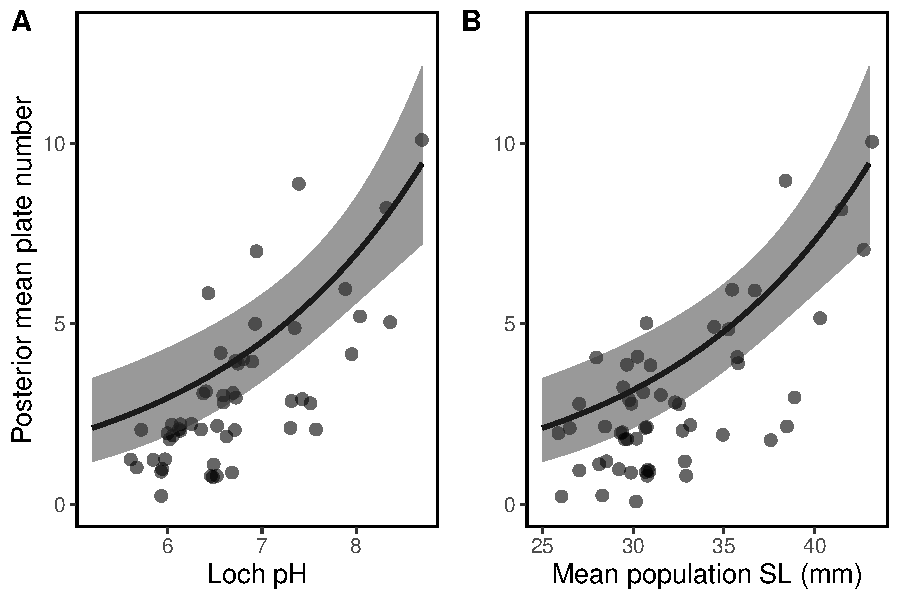
\includegraphics{Bayesian_GLMs_files/figure-latex/ch5-final-plot-1} 

}

\caption{\textbf{Posterior mean lateral plate number of three-spined stickleback populations on North Uist as a function of: A. loch pH; B. mean population standard length (mm), modelled using a Poisson GLM fitted with INLA. Shaded areas are Bayesian 95\% credible intervals. Black points are observed data for different stickleback populations.}}\label{fig:ch5-final-plot}
\end{figure}

The results of this statistical analysis can be summarised as follows:

\emph{A Poisson GLM was fitted to data using Bayesian inference with INLA for lateral plate counts of three-spined sticklebacks from 57 populations on North Uist, Scotland. An Information Theoretic approach was adopted for model fitting, with nine alternative models formulated that comprised variables proposed as having importance as environmental agents of selection on lateral plate number in previously published studies (Table 5.7). In the best-fitting model there was a statistically important positive effect of loch pH and mean population standard length (in mm) (Table 5.7, Fig. \ref{fig:ch5-final-plot}). The mean slope of the relationship between plate number and pH was 0.44 with 95\% certainty that it lay between 0.25 and 0.62, and for standard length 0.054 with 95\% certainty that it lay between 0.018 and 0.091 (Table 5.7). The model was fitted using informative priors on the fixed effects, obtained from a separate study of three-spined stickleback plate number derived from the entire European range of the species (Table 5.2).}

\hypertarget{conclusions-2}{%
\section{Conclusions}\label{conclusions-2}}

In this analysis we used an Information Theoretic (IT) approach to choose among a set of biologically plausible models, in combination with informative priors based on existing data collected over a wide geographic range. The final Poisson GLM predicted three-spined stickleback lateral plate number on North Uist to vary positively as a function of loch pH and mean population standard length.

\hypertarget{nb-glm}{%
\chapter{Bayesian negative binomial GLM}\label{nb-glm}}

A negative binomial GLM is used for the same type of data that a Poisson GLM would be used to analyse; count data that does not take values below zero. However, the negative binomial GLM does not assume that the variance of the response variable is equal to its mean and, therefore, can be used to model overdispersed data, which is a common property of ecological data. Formulation of a Bayesian negative binomial GLM is slightly more complex than the Bayesian Poisson GLM presented in Chapter \ref{pois-glm}, and a negative binomial GLM is typically used when a Poisson GLM is not appropriate due to overdispersion.

\hypertarget{coral-abundance}{%
\section{Coral abundance}\label{coral-abundance}}

We fit a GLM to data on coral diversity in the Sulu Sea off the North coast of Borneo. Surveys of Scleractinia (hard coral) species were conducted on reefs inside and outside a marine protected area established 5 years previously. Surveys were conducted at specific depths, ranging from 3-10 m. A randomly demarcated area of 100 m\textsuperscript{2} was comprehensively searched by a pair of divers and the number of coral species recorded on a slate board. All coral species were photographed to confirm \emph{in situ} identification using a reference collection. Survey sites were at least 8 km apart and were surveyed only once.

Here we analyse data on coral diversity on reefs inside and outside a protected area while controlling for water depth, which is a variable known to have a strong effect on coral diversity. The aim of the study was to understand the short-term impact of implementing a marine protected area in zones from which all fishing and tourism was prohibited.

\emph{\textbf{Import data}}

Data for coral diversity are saved in a comma-separated values (CSV) file coral.csv and are imported into a dataframe in R using:

\texttt{coral\ \textless{}-\ read\_csv("coralsulu.csv")}

Start by inspecting the dataframe:

\texttt{str(coral)}

\begin{verbatim}
spec_tbl_df [32 x 4] (S3: spec_tbl_df/tbl_df/tbl/data.frame)
 $ site   : num [1:32] 1 2 3 4 5 ...
 $ status : chr [1:32] "protected" "unprotected" ...
 $ depth  : num [1:32] 8 4 5 6 8 ...
 $ species: num [1:32] 50 52 86 63 49 ...
 - attr(*, "spec")=
  .. cols(
  ..   site = col_double(),
  ..   status = col_character(),
  ..   depth = col_double(),
  ..   species = col_double()
  .. )
\end{verbatim}

The dataframe comprises 32 observations of 4 variables. Each row in the dataframe represents a separate surveyed reef (\texttt{site}). There is a single categorical variable \texttt{status} which indicates whether the reef was a protected or unprotected site. There are two continuous ecological variables: \texttt{depth} is water depth (in m) for each surveyed reef, and \texttt{species} is the number of scleractinian coral species.

\hypertarget{nb-glm-steps}{%
\section{Steps in fitting a Bayesian GLM}\label{nb-glm-steps}}

We will following the 9 steps to fitting a Bayesian GLM, detailed in Section \ref{fit-steps}.

\emph{1. State the question}

\emph{2. Perform data exploration}

\emph{3. Select a statistical model}

\emph{4. Specify and justify a prior distribution on parameters}

\emph{5. Fit the model}

\emph{6. Obtain the posterior distribution}

\emph{7. Conduct model checks}

\emph{8. Interpret and present model output}

\emph{9. Visualise the results}

\hypertarget{coral-question}{%
\subsection{State the question}\label{coral-question}}

This study was conducted to ascertain the benefit of implementing a marine protected area on coral diversity. The variable \texttt{species} is the response variable and conservation status (\texttt{status}) is a categorical covariate. Because there is a well recognised negative relationship of water depth on coral species abundance (i.e.~coral diversity is greater in shallow water), water depth (\texttt{depth}) is an additional continuous covariate. Further, the effect of reef protected status may vary with water depth, particularly in the case of the impact of tourists who tend to cause most damage to corals in shallow water. Consequently, the interaction of \texttt{status} and \texttt{depth} on coral diversity (\texttt{species}) will also be included in a model.

\hypertarget{coral-eda}{%
\subsection{Data exploration}\label{coral-eda}}

A data exploration is critical to identifying any potential problems or unusual patterns in the data. First check for missing data.

\texttt{colSums(is.na(coral))}

\begin{verbatim}
   site  status   depth species 
      0       0       0       0 
\end{verbatim}

There are no missing data.

\hypertarget{coral-outliers}{%
\subsubsection{Outliers}\label{coral-outliers}}

Outliers in the data can identified visually using Cleveland dotplots, R code is available in the R script associated with this chapter:



\begin{figure}

{\centering 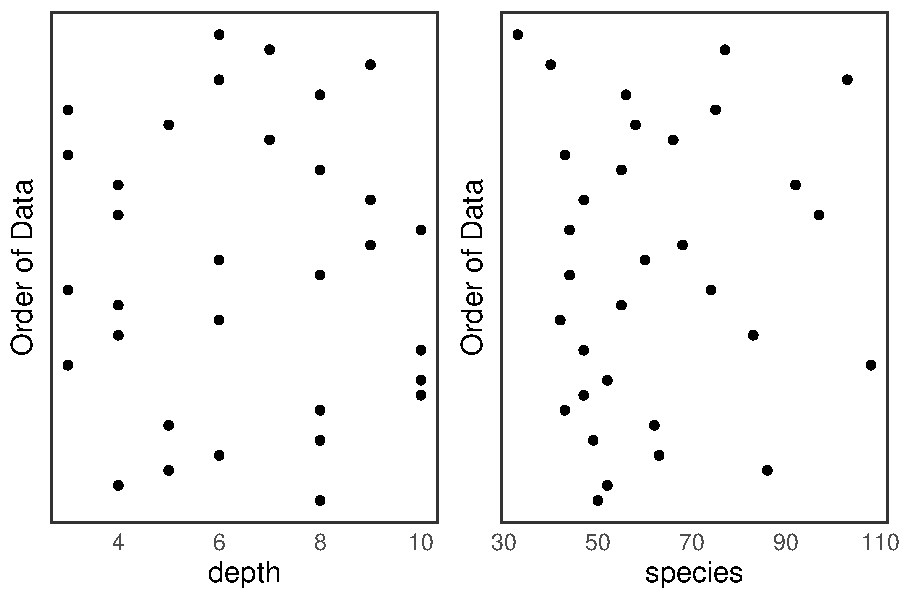
\includegraphics{Bayesian_GLMs_files/figure-latex/ch6-dotplot-1} 

}

\caption{\textbf{Dotplots of water depth (m) and number of hard coral species at sampling sites in the Sulu Sea. Data are arranged by the order they appear in the dataframe.}}\label{fig:ch6-dotplot}
\end{figure}

There are no obvious outliers in the Fig. \ref{fig:ch6-dotplot}.

\hypertarget{nb-dist}{%
\subsubsection{Distribution of the dependent variable}\label{nb-dist}}

The distribution of the dependent variable will inform selection of the appropriate statistical model to use. Here we visualise coral species number with a density plot using the \texttt{geom\_density()} function from the \texttt{ggplot2} package:

\texttt{coral\ \%\textgreater{}\%\ ggplot(aes(species))\ +\ geom\_density()\ +\ xlab\ \ ("Number\ of\ coral\ species")\ +\ ylab("Density")\ +\ xlim(25,125)\ +\ My\_theme\ +\ theme(panel.border\ =\ element\_rect(colour\ =\ "black",\ fill=NA,\ size\ =\ 1))}



\begin{figure}

{\centering 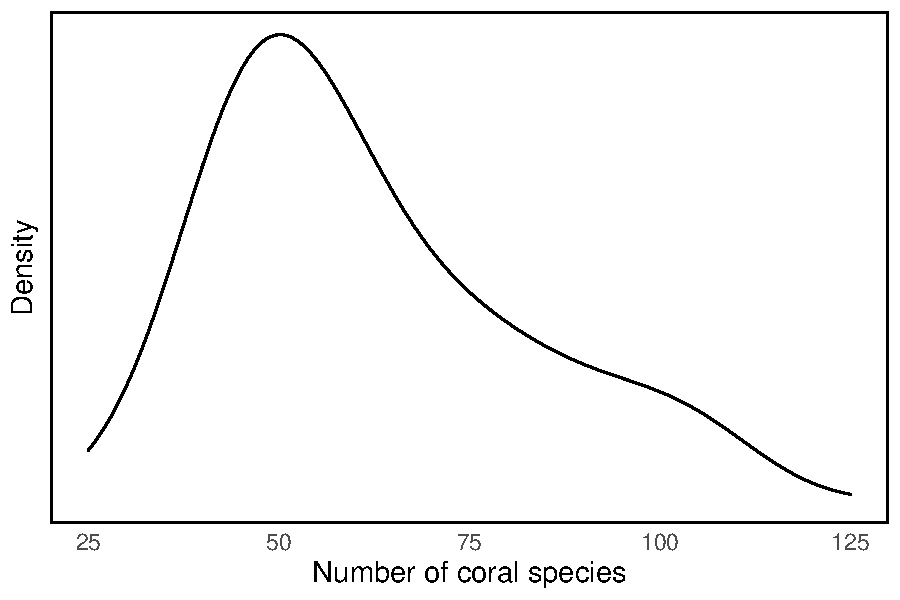
\includegraphics{Bayesian_GLMs_files/figure-latex/ch6-freqdens-1} 

}

\caption{\textbf{Density plot of number of coral species from 32 surveyed reefs.}}\label{fig:ch6-freqdens}
\end{figure}

The density plot of the dependent variable (Fig. \ref{fig:ch6-freqdens}) shows a distribution with a pronounced positive skew.

\hypertarget{nb-balance}{%
\subsubsection{Balance of categorical variables}\label{nb-balance}}

The balance of the categorical variables status (the protected status of surveyed reefs) can be checked using the \texttt{table()} function.

\texttt{table(coral\$status)}

\begin{verbatim}
  protected unprotected 
         16          16 
\end{verbatim}

The design of the study is perfectly balanced.

\hypertarget{nb-collin}{%
\subsubsection{Multicollinearity among covariates}\label{nb-collin}}

If covariates in a model are correlated, then there is a risk that the model may produce unstable parameter estimates with inflated standard errors. Here we examine the relationships among model covariates using the \texttt{ggpairs} command from the \texttt{GGally} library (see R code associated with this chapter).



\begin{figure}

{\centering 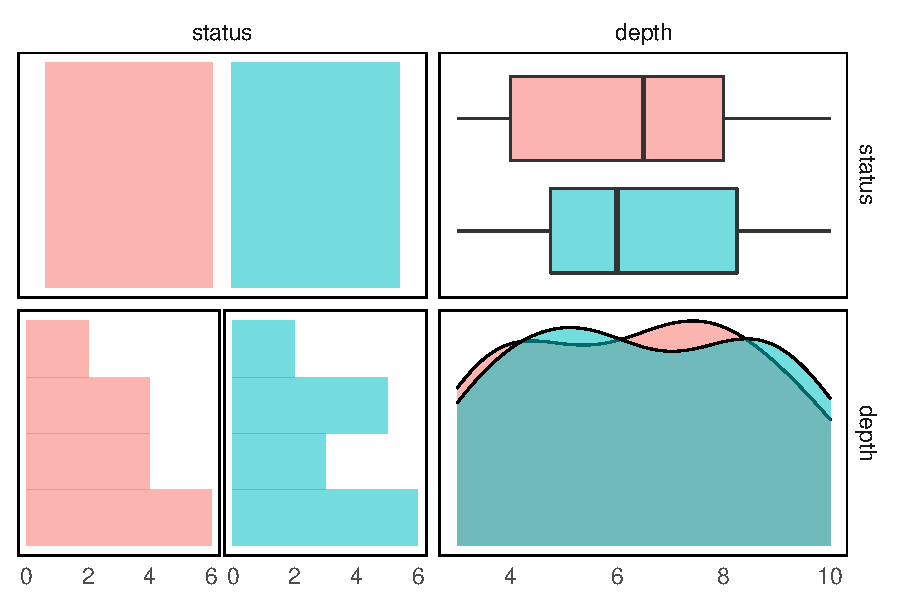
\includegraphics{Bayesian_GLMs_files/figure-latex/ch6-ggpairs-1} 

}

\caption{\textbf{Plot matrix of covariates showing frequency plots, boxplots, frequency histograms, and frequency polygons.}}\label{fig:ch6-ggpairs}
\end{figure}

The plot matrix in Fig. \ref{fig:ch6-ggpairs} indicates no evidence of collinearity.

\hypertarget{nb-zeros}{%
\subsubsection{Zeros in the response variable}\label{nb-zeros}}

The number of zeros in the response variable needs to be considered and will inform selection of the appropriate statistical model. The percentage of zeros in the response variable can be calculated with:

\texttt{round((sum(coral\$species\ ==\ 0)\ /\ nrow(coral))*100,0)}

0

The response variable does not include any zeros.

\hypertarget{nb-rels}{%
\subsubsection{Relationships among dependent and independent variables}\label{nb-rels}}

Visual inspection of the data using plots will illustrate the nature of relationships among covariates (code for the plot is available in the R script associated with this chapter):



\begin{figure}

{\centering 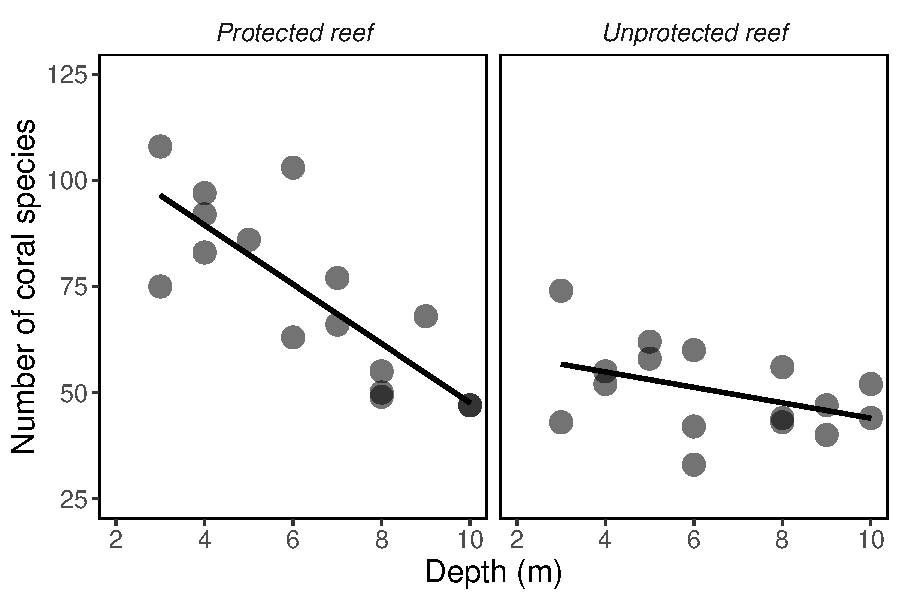
\includegraphics{Bayesian_GLMs_files/figure-latex/ch6-scatter-1} 

}

\caption{\textbf{Multipanel scatterplot of number of coral species against water depth for protected and unprotected reefs with a line of best fit plotted.}}\label{fig:ch6-scatter}
\end{figure}

The plots in Fig. \ref{fig:ch6-scatter} suggest a negative relationship between the number of coral species and water depth, with this relationship stronger for protected than unprotected reefs, which implies a protected status x depth interaction.

\hypertarget{nb-indep}{%
\subsubsection{Independence of response variable}\label{nb-indep}}

An assumption for a GLM is that each observation in a dataset is independent of all others. In the case of the present study each row of data represents data from a survey of a geographically discrete reef, with reefs a minimum of 8 km apart. Ostensibly then, these data were independent. However, there is the potential for spatial dependency in the data based on their location. A GLM does not permit spatial (or temporal) dependency to be adequately modelled and so, for the purposes of this analysis, while we will treat the data as independent, though that may not strictly be the case.

\hypertarget{nb-select}{%
\subsection{Selection of a statistical model}\label{nb-select}}

The study was designed to gauge the effect of implementing protection measures on coral biodiversity. The dependent variable comprises coral species counts that potentially includes zero, though negative values are not possible. The distribution of the response variable is positively skewed (Fig. \ref{fig:ch6-freqdens}). The data will treated as independent, though there is the potential for spatial dependency in the data.

Given these circumstances, a Poisson is an appropriate distribution as a starting point to model the data, in combination with a log link function. The Poisson is a non-normal distribution that is effective for modelling strictly positive integer data (such as counts). It has a single parameter (lambda, \(\lambda\)), which is both the mean and variance of the response variable. In the context of an INLA model, a Poisson model has no hyperparameter.

The link function is used to link the response variable (number of coral species) and the predictor function (protected status and water depth). In the case of a Poisson GLM the default is a log link function. The link function is needed to ensure model fitted values remain positive, while permitting zeros in the data.

\hypertarget{nb-prior-spec}{%
\subsection{Specification of priors}\label{nb-prior-spec}}

Informative priors used in this study come from a previous similar study from the same region by \citet{Waheed_2015}.

\hypertarget{previous-study}{%
\subsubsection{Previous study}\label{previous-study}}

In \citet{Waheed_2015} coral diversity was modelled using a Poisson GLM with depth, exposure and distance to mainland as covariates. This model provides informative priors for model intercept and depth, but not for protected status. However, numerous other studies from several tropical regions have consistently demonstrated a positive effect of protected status on coral reef biodiversity, which enables us to confidently place weakly informative priors on the effect of reef protected status and its interaction with depth.

\hypertarget{nb-priors-fixed}{%
\subsubsection{Priors on the fixed effects}\label{nb-priors-fixed}}

Non-informative (default) priors were put on the fixed effects for model \texttt{M01}, which were:

\(\beta intercept\) \textasciitilde{} \emph{N}(0, 0) (\(\tau\) = 0)

\(\beta depth\) \textasciitilde{} \emph{N}(0, 1000) (\(\tau\) = 0.001)

\(\beta statusunprotected\) \textasciitilde{} \emph{N}(0, 1000) (\(\tau\) = 0.001)

\(\beta interaction\) \textasciitilde{} \emph{N}(0, 1000) (\(\tau\) = 0.001)

And informative/weakly informative priors on the fixed effects for model \texttt{I01}:

\(\beta intercept\) \textasciitilde{} \emph{N}(5, 0.25) (\(\tau\) = 4)

\(\beta depth\) \textasciitilde{} \emph{N}(-0.18, 0.0036) (\(\tau\) = 278)

\(\beta statusunprotected\) \textasciitilde{} \emph{N}(-0.5, 0.0625) (\(\tau\) = 16)

\(\beta interaction\) \textasciitilde{} \emph{N}(0.05, 1) (\(\tau\) = 1)

The prior for the intercept comes from \citet{Waheed_2015}, who present a model intercept of 3.8 (\(\sigma\) = 0.08). Here we round the intercept to 5, with \(\sigma\) = 0.5, to generate a weakly informative prior. We use an informative prior for the slope of depth from \citet{Waheed_2015} of -0.18 (\(\sigma\) = 0.06). An informative prior is also used for protected status, with a slope of -0.5 (\(\sigma\) = 0.25) for unprotected sites. For the interaction term we use a weakly informative positive prior of 0.05 (\(\sigma\) = 1).

\hypertarget{nb-fit-models}{%
\subsection{Fit the models}\label{nb-fit-models}}

We fit the Bayesian Poisson GLMs using INLA with default priors (M01), and informative priors on the fixed effects (I01).

We start by specifying the model formulae:

\texttt{f01\ \textless{}-\ species\ \textasciitilde{}\ depth\ *\ status}

Then fit the default model \texttt{M01}, specifying \texttt{control.compute\ =\ list(dic\ =\ TRUE)} to enable model comparison:

\texttt{M01\ \textless{}-\ inla(f01,\ control.compute\ =\ list(dic\ =\ TRUE),\ family\ =\ "poisson",\ data\ =\ coral)}

Then fit the model with informative priors:

\texttt{I01\ \textless{}-\ inla(f01,\ family\ =\ "poisson",\ data\ =\ coral,\ control.\ compute\ =\ list(dic\ =\ TRUE),\ control.fixed\ =\ list(mean.\ intercept\ =\ 5.0,\ prec.intercept\ =\ 0.5\^{}(-2),\ mean\ =\ list(depth\ =\ -0.18,\ statusunprotected\ =\ -0.5,\ default\ =\ 0.05),\ prec\ =\ list(depth\ =\ 0.06\^{}(-2),\ statusunprotected\ =\ 0.25\^{}(-2),\ default\ =\ 1\^{}(-2))))}

\hypertarget{nb-post-dist}{%
\subsection{Obtain the posterior distribution}\label{nb-post-dist}}

\hypertarget{nb-def-priors}{%
\subsubsection{Model with default priors}\label{nb-def-priors}}

Output for the fixed effects of M01 can be obtained with:

\texttt{M01Betas\ \textless{}-\ M01\$summary.fixed{[},c("mean",\ "sd",\ "0.025quant",\ "0.975quant"){]}}

\texttt{round(M01Betas,\ digits\ =\ 2)}

\begin{verbatim}
                         mean   sd 0.025quant 0.975quant
(Intercept)              4.88 0.08       4.72       5.04
depth                   -0.10 0.01      -0.12      -0.07
statusunprotected       -0.73 0.13      -0.99      -0.48
depth:statusunprotected  0.06 0.02       0.02       0.10
\end{verbatim}

This reports the posterior mean, standard deviation and 95\% credible intervals for the intercept and covariates.

For the slope of the variable depth we have a posterior mean of -0.10 and lower 95\% credible interval of -0.12 and upper 95\% credible interval of -0.07; we are 95\% certain that the posterior mean of the regression parameter for the slope of depth falls between these credible intervals, which means depth is statistically important in the model.

We can similarly conclude that the effect of the protected status of a reef has an important effect on coral species biodiversity, and is lower for unprotected reefs. There is also an important effect of a depth x status interaction in the data.

The posterior distribution of the fixed effects can be visualised using \texttt{ggplot2.} The coding for this plot is available in the R script associated with this chapter.



\begin{figure}

{\centering 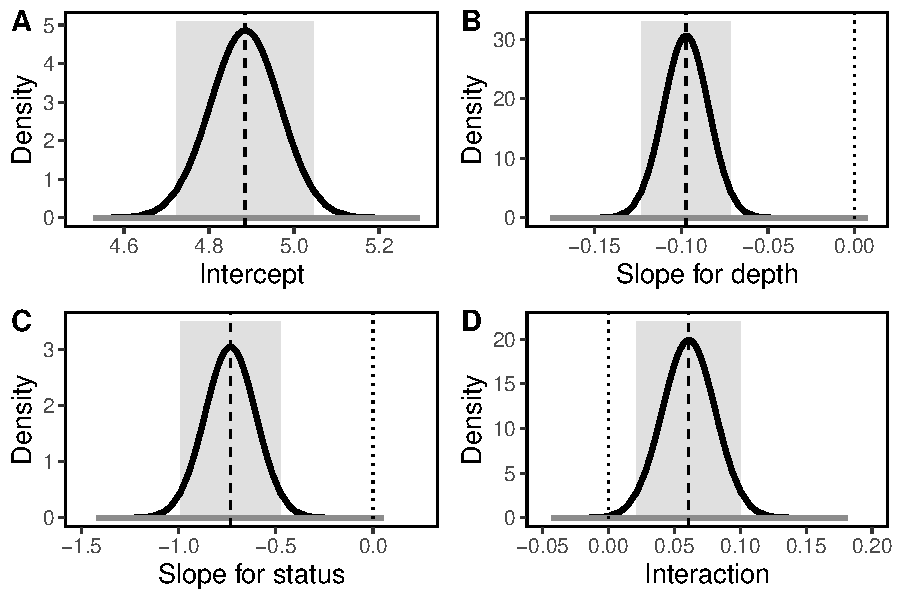
\includegraphics{Bayesian_GLMs_files/figure-latex/ch6-M01-betas-1} 

}

\caption{\textbf{Posterior and prior distributions for fixed parameters of a Bayesian Poisson GLM to model the number of coral species. The model is fitted with default (non-informative) priors. Distributions for: A. model intercept; B. slope for depth; C. slope for reef status; D. interaction of depth and reef status. The solid black line is the posterior distribution, the solid gray line is the prior distribution, the gray shaded area encompasses the 95\% credible intervals, the vertical dashed line is the posterior mean of the parameter, the vertical dotted line indicates zero. For parameters where zero (indicated by dotted line) falls outside the range of the 95\% credible intervals (gray shaded area), the parameter is statistically important.}}\label{fig:ch6-M01-betas}
\end{figure}

Figure \ref{fig:ch6-M01-betas} provides a visual representation of the summary of the fixed effects, and indicates that for model \texttt{M01} the betas for the intercept and for depth, protected status and interaction between depth and protected status are statistically important. This figure also shows the non-informative priors make a limited contribution to the posterior distribution.

\hypertarget{nb-inf-priors}{%
\subsubsection{Model with informative priors}\label{nb-inf-priors}}

As for the default model, we will examine the posterior distributions for the model with informative/weakly informative priors.

\texttt{I01Betas\ \textless{}-\ I01\$summary.fixed{[},c("mean",\ "sd",\ "0.025quant",\ "0.975quant"){]}}

\texttt{round(I01Betas,\ digits\ =\ 2)}

\begin{verbatim}
                         mean   sd 0.025quant 0.975quant
(Intercept)              4.89 0.08       4.74       5.04
depth                   -0.10 0.01      -0.12      -0.07
statusunprotected       -0.70 0.11      -0.93      -0.48
depth:statusunprotected  0.06 0.02       0.02       0.09
\end{verbatim}

The qualitative outcome for the informative model is the same as the model with default priors, with all betas statistically important. However, posterior means differ quantitatively from the model with default priors, as do the 95\% credible intervals which encompass a narrower range. The posterior distributions can be visualized with \texttt{ggplot2}: see the R script associated with this chapter.



\begin{figure}

{\centering 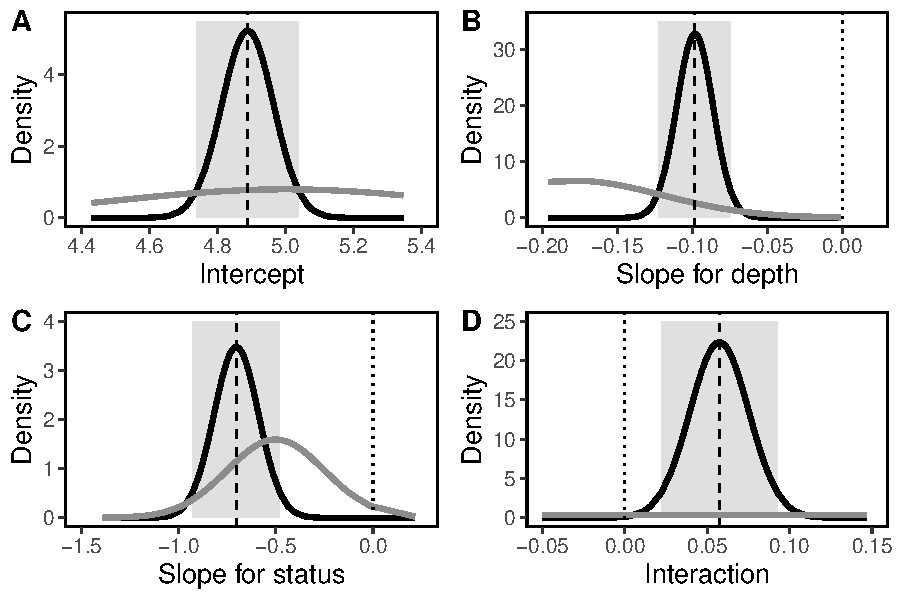
\includegraphics{Bayesian_GLMs_files/figure-latex/ch6-I01-betas-1} 

}

\caption{\textbf{Posterior and prior distributions for fixed parameters of a Bayesian Poisson GLM to model the number of coral species. The model is fitted with informative priors. Distributions for: A. model intercept; B. slope for depth; C. slope for reef status; D. interaction of depth and reef status. The solid black line is the posterior distribution, the solid gray line is the prior distribution, the gray shaded area encompasses the 95\% credible intervals, the vertical dashed line is the posterior mean of the parameter, the vertical dotted line indicates zero. For parameters where zero (indicated by dotted line) falls outside the range of the 95\% credible intervals (gray shaded area), the parameter is statistically important.}}\label{fig:ch6-I01-betas}
\end{figure}

Figure \ref{fig:ch6-I01-betas} indicates that for model I01 the betas for the intercept, depth, reef protected status and interaction between depth and protected status all differ from zero and are statistically important. Note that the priors for depth and protected status are informative; these are based on the comparable previous study by \citet{Waheed_2015}. Priors for the model intercept and interaction are weakly informative.

\hypertarget{nb-prior-comp}{%
\subsubsection{Comparison of models with uninformative and informative priors}\label{nb-prior-comp}}

We can compare the results of the Bayesian Poisson GLM with uninformative priors with the same model fitted with informative priors using the DIC.

First extract DICs:

\texttt{InfDIC\ \textless{}-\ c(M01\$dic\$dic,\ I01\$dic\$dic)}

Add weighting:

\texttt{InfDIC.weights\ \textless{}-\ aicw(InfDIC)}

Add names:

\texttt{rownames(InfDIC.weights)\ \textless{}-\ c("default","informative")}

Print DICs:

\texttt{dprint.inf\ \textless{}-\ print\ (InfDIC.weights,\ abbrev.names\ =\ FALSE)}

Order DICs by fit:

\texttt{round(dprint.inf{[}order(dprint.inf\$fit),{]},2)}

\begin{verbatim}
                 fit     delta         w
default     252.6308 0.4286121 0.4466276
informative 252.2022 0.0000000 0.5533724
\end{verbatim}

\begin{verbatim}
               fit delta    w
informative 252.20  0.00 0.55
default     252.63  0.43 0.45
\end{verbatim}

These DIC score are essentially the same.

\hypertarget{nb-freq-comp}{%
\subsubsection{Comparison with frequentist Poisson GLM}\label{nb-freq-comp}}

We can compare the results of the Bayesian Poisson GLMs with the same model fitted in a frequentist setting. Execution of the model in a frequentist framework can be performed with:

\texttt{Freq\ \textless{}-\ glm(species\ \textasciitilde{}\ depth\ *\ status,family\ =\ "poisson",\ data\ =\ coral)}

\texttt{round(summary(Freq)\$coef{[},1:4{]},2)}

\begin{verbatim}
                        Estimate Std. Error z value Pr(>|z|)
(Intercept)                 4.88       0.08   59.53        0
depth                      -0.10       0.01   -7.45        0
statusunprotected          -0.73       0.13   -5.59        0
depth:statusunprotected     0.06       0.02    3.04        0
\end{verbatim}

We can compare these with the results for the Bayesian models:

Table 6.1: \textbf{Comparison of model parameters for frequentist, Bayesian model with non-informative and informative priors of Poisson GLM model to investigate the number of hard coral species on reefs in the Sulu Sea.}

\begin{longtable}[]{@{}lcccc@{}}
\toprule
Model & Intercept & depth & status & interaction \\
\midrule
\endhead
Frequentist & 4.88(0.08) & -0.10(0.01) & -0.73(0.13) & -0.06(0.02) \\
Bayesian (default) & 4.88(0.08) & -0.10(0.01) & -0.73(0.13) & -0.06(0.02) \\
Bayesian (informative) & 4.89(0.08) & -0.10(0.01) & -0.73(0.13) & -0.06(0.02) \\
\bottomrule
\end{longtable}

Parameter estimates for the frequentist and Bayesian model with non-informative priors are identical, while results for the Bayesian model with informative priors differ only slightly.

\hypertarget{conduct-model-checks-2}{%
\subsection{Conduct model checks}\label{conduct-model-checks-2}}

After model fitting and obtaining the posterior distributions, a next step is validation of the model through model checks.

\hypertarget{nb-dic}{%
\subsubsection{Model selection using the Deviance Information Criterion (DIC)}\label{nb-dic}}

We perform a simple model selection by removing covariates and comparing models using the DIC. Start by formulating alternative model:

\texttt{f01\ \textless{}-\ species\ \textasciitilde{}\ depth\ *\ status}

\texttt{f02\ \textless{}-\ species\ \textasciitilde{}\ depth\ +\ status}

\texttt{f03\ \textless{}-\ species\ \textasciitilde{}\ depth}

\texttt{f04\ \textless{}-\ species\ \textasciitilde{}\ status}

To use DIC we must re-fit the model and specify its calculation using \texttt{control.compute}.

Full model with default priors:

\texttt{M01.full\ \textless{}-\ inla(f01,\ control.compute\ =\ list(dic\ =\ TRUE),\ family\ =\ "poisson",\ data\ =\ coral)}

Model with default priors with interaction dropped:

\texttt{M01.1\ \textless{}-\ inla(f02,\ control.compute\ =\ list(dic\ =\ TRUE),\ family\ =\ "poisson",\ data\ =\ coral)}

Model with default priors with reef status dropped:

\texttt{M01.2\ \textless{}-\ inla(f03,\ control.compute\ =\ list(dic\ =\ TRUE),\ family\ =\ "poisson",\ data\ =\ coral)}

Model with default priors with depth dropped:

\texttt{M01.3\ \textless{}-\ inla(f04,\ control.compute\ =\ list(dic\ =\ TRUE),\ family\ =\ "poisson",\ data\ =\ coral)}

Compare models with the DIC:

\texttt{M01dic\ \textless{}-\ c(M01.full\$dic\$dic,\ M01.1\$dic\$dic,M01.2\$dic\$dic,\ \ \ \ M01.3\$dic\$dic)}

\texttt{DIC\ \textless{}-\ cbind(M01dic)}

\texttt{rownames(DIC)\ \textless{}-\ c("full","no\ inter","no\ status","no\ depth")}

\texttt{round(DIC,0)}

\begin{verbatim}
          M01dic
full         253
no inter     260
no status    321
no depth     311
\end{verbatim}

The full model is the best fitting.

We repeat the same process with the model with informative priors (coding is available in the R script associated with this chapter) which gives:

\begin{verbatim}
          I01dic
full         252
no inter     260
no status    321
no depth     311
\end{verbatim}

Which gives the same outcome as the model with default priors. Given the similarity in the models with noninformative and informative priors, for brevity we choose to continue model checks with just the latter model.

\hypertarget{nb-disp}{%
\subsubsection{Dispersion}\label{nb-disp}}

A necessary check with a Poisson GLM is whether it is overdispersed. Dispersion can be assessed by summing the squared Pearson residuals and dividing them by the number of observations minus the degrees of freedom. This value should be close to one. Values above one indicate overdispersion, while values below one indicate underdispersion.

However this approach is rather arbitrary and a better comparison for assessing dispersion is to simulate data from the fitted model and calculate the dispersion for each of the simulated data sets.

In Chapter 5 we implemented the 7-step protocol of \citet{Zuur_2017} to assess dispersion in the Poisson GLM with informative priors. Here we conduct an alternative simulation using the \texttt{inlatools} package.

We start by refitting the model with the \texttt{config\ =\ TRUE} option to permit the simulation of regression parameters:

\texttt{I01\ \textless{}-\ inla(f01,\ family\ =\ "poisson",\ data\ =\ coral,\ control.\ compute\ =\ list(config\ =\ TRUE,\ dic\ =\ TRUE),\ control.predictor\ =\ list(compute\ =\ TRUE),\ control.fixed\ =\ list(mean.intercept\ =\ 5.0,\ prec.intercept\ =\ 0.5\^{}(-2),\ mean\ =\ list(depth\ =\ -0.18,\ statusunprotected\ =\ -0.5,\ default\ =\ 0.05),\ prec\ =\ list(depth\ =\ 0.06\^{}(-2),\ statusunprotected\ =\ 0.25\^{}(-2),\ default\ =\ 1\^{}(-2))))}

We simulate data from the model with \texttt{dispersion\_check}:

\texttt{dis\_pois\ \textless{}-\ dispersion\_check(I01)}

Which generates the dispersion value based on the data and a vector of dispersion values for 1000 simulated data sets

The dispersion value for the data is given by:

\texttt{round(dis\_pois\$data,2)}

\begin{verbatim}
[1] 1.73
\end{verbatim}

This figure should be close to 1 (\textless1 underdispersion, \textgreater1 overdispersion). However, the value for the model exceeds 1, indicating a problem of overdispersion.

We can plot dispersion values for the simulated data sets (with dispersion value for the data added as a dashed line)

\texttt{pois\_plot\ \textless{}-\ ggplot()\ +\ geom\_density(aes(dis\_pois\$model))\ +\ geom\_vline(xintercept\ =\ dis\_pois\$data,\ linetype\ =\ "dashed")\ +\ xlab("Dispersion")\ +\ ylab("Density")\ +\ xlim(0,2.1)\ +\ ylim(0,1.8)\ +\ theme(text\ =\ element\_text(size=13))\ +\ theme(panel.background\ =\ element\_blank())\ +\ theme(panel.\ border\ =\ element\_rect(fill\ =\ NA,\ colour\ =\ "black",\ size\ =\ 1))\ +\ theme(strip.background\ =\ element\_rect\ (fill\ =\ "white",\ color\ =\ "white",\ size\ =\ 1))}

\texttt{pois\_plot}



\begin{figure}
\centering
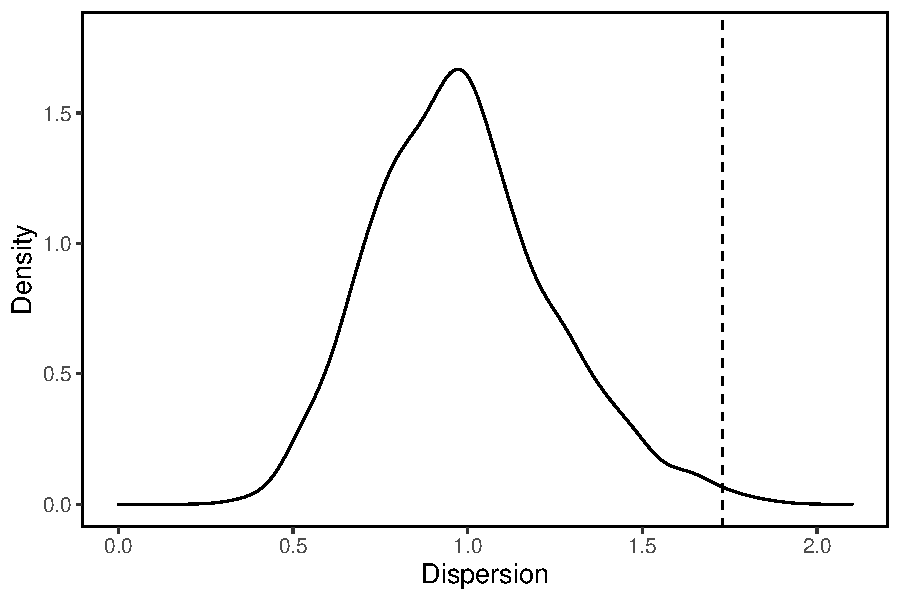
\includegraphics{Bayesian_GLMs_files/figure-latex/ch6-pois-plot-1.pdf}
\caption{\label{fig:ch6-pois-plot}\textbf{Density plot of the dispersion of the simulated data sets. The vertical dashed line shows the dispersion of the original data.}}
\end{figure}

If the dispersion value for the data (dashed line) in Fig. \ref{fig:ch6-pois-plot} falls within the distribution of dispersion values for simulated data sets the model is not under- or overdispersed. However, in this case there is clear evidence of overdispersion.

\emph{\textbf{Overdispersion}}

Poisson GLMs assume the mean and variance of the response variable are approximately equal. Overdispersion can occur when this assumption is not met; variance in the data is naturally larger than the mean. This situation is termed `true overdispersion'. True overdispersion is dealt with by fitting a model to the data such that the variance is greater than the mean in the response variable.

However, there are other possible causes of overdispersion, which can represent underlying problems with the model. These are:

\begin{enumerate}
\def\labelenumi{\arabic{enumi}.}
\item
  \textbf{Model mis-specification}. There may be key variables, including interactions, that explain a large part of the variance that are missing from the model. Model mis-specification is handled by including additional variables or adding interaction terms to the model.
\item
  \textbf{Too many zeros in the response variable (`zero inflation')}. If there are too many zeros a zero-inflated (e.g.~a zero-inflated Poisson or ZIP model) or zero-adjusted (e.g.~a zero-adjusted Poisson or ZAP) model can be used.
\item
  \textbf{Influential outliers}. The presence of influential observations can be tested by plotting Cook's distance and these can be dropped and the model refitted. Data dropped from the analysis must be reported in your Methods, with a justification.
\item
  \textbf{Non-independence of the data}. An assumption is that each observation in a dataset is independent of all others. However, there may be an underlying association between some data that results in dependency; e.g.~data may have been collected by different scientists, who introduce consistent bias to the data, or data may have been collected in different months, which affects the variance structure of the data. If the source of dependency is known, it can be incorporated into the analysis as a `random' term in a Generalised Linear Mixed Model (GLMM).
\item
  \textbf{Wrong link function}. A GLM uses a link function to connect the response variable with the linear part of the model comprising the covariates. Trying an alternative link function to the default may solve the problem of overdispersion.
\item
  \textbf{Non-linearity in the data}. A GLM assumes the response variable can be modelled as a linear relationship using a link function. However, this approach may not be adequate to capture the non-linear properties of some biological systems. In this case it is necessary to switch to using Generalised Additive Models (GAMs).
\end{enumerate}

As part of model validation, it is necessary to address each of these potential problems. If none prove successful in solving overdispersion, a model with a different error structure can be applied.

To see a full assessment of these steps, see Chapter 8 of \citep{Smith_etal_2020} with accompanying R script. In the case of the coral data we found no evidence for any of these alternative causes of overdispersion and we will assume that there is true overdispersion in the data; i.e.~variance in the data is naturally larger than the mean and a model with a different conditional probability distribution is needed.

\hypertarget{nbglm-fit}{%
\subsubsection{Bayesian negative binomial GLM}\label{nbglm-fit}}

We will refit model \texttt{I01} with a negative binomial distribution for the response variable. The negative binomial distribution is a generalisation of the Poisson that relaxes the restrictive assumption that the variance is equal to the mean. Instead, the variance of a negative binomial GLM is modelled as a function of its mean and a dispersion parameter.

Fitting a negative binomial GLM is readily achieved in INLA by simply altering the model family from \texttt{poisson} to \texttt{nbinomial}:

\texttt{I01.nb\ \textless{}-\ inla(f01,\ family\ =\ "nbinomial",\ data\ =\ coral,\ control.\ \ compute\ =\ list(config\ =\ TRUE,\ dic\ =\ TRUE),\ control.\ \ predictor\ =\ list(compute\ =\ TRUE),\ control.fixed\ =\ list(mean.intercept\ =\ 5.0,\ prec.intercept\ =\ 0.5\^{}(-2),\ mean\ =\ list(depth\ =\ -0.18,\ \ statusunprotected\ =\ -0.5,\ default\ =\ 0.05),\ prec\ =\ list(depth\ =\ 0.06\^{}(-2),\ status\ \ unprotected\ =\ 0.25\^{}(-2),\ default\ =\ 1\^{}(-2))))}

Then repeat the simulation exercise with the negative binomial GLM:

\texttt{dis\_nbin\ \textless{}-\ dispersion\_check(I01.nb)}

The dispersion value for the data is given by:

\texttt{round(dis\_nbin\$data,2)}

\begin{verbatim}
[1] 1.16
\end{verbatim}

This figure should be close to 1, which is the case.

We can also plot the dispersion and compare with the Poisson GLM (R code is available in the R script associated with this chapter):



\begin{figure}

{\centering 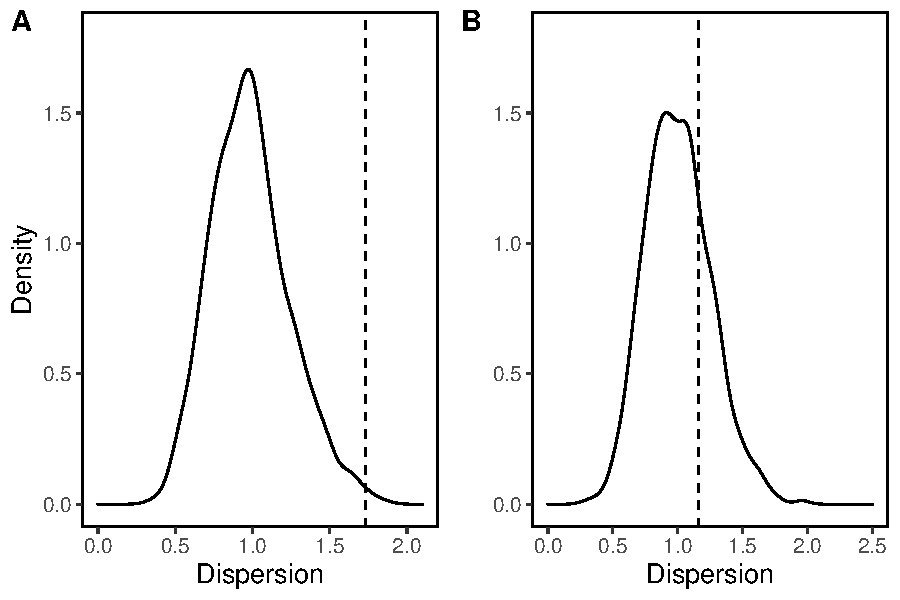
\includegraphics{Bayesian_GLMs_files/figure-latex/ch6-nbglm-plot-1} 

}

\caption{\textbf{Density plot of the dispersion of the simulated data sets for: A. Poisson model; B. negative binomial model. The vertical dashed line shows the dispersion of the data.}}\label{fig:ch6-nbglm-plot}
\end{figure}

In Fig. \ref{fig:ch6-nbglm-plot} the dispersion value for the data (dashed line) fitted with a Poisson distribution (panel A) falls outside the distribution of dispersion values for the simulated data sets, indicating overdispersion, while for the negative binomial distribution (panel B) the dispersion value clearly falls within the distribution of the dispersion values for the simulated data sets. This outcome shows that the implementation of a negative binomial distribution has adequately handled the problem of overdispersion, and this negative binomial model will be used for further model checks.

We can also compare DICs for the Poisson and negative binomial models:

\texttt{dic3\ \textless{}-\ c(I01\$dic\$dic,\ I01.nb\$dic\$dic)}

\texttt{DIC3\ \textless{}-\ cbind(dic3)}

\texttt{rownames(DIC3)\ \textless{}-\ c("Poisson","negative\ binomial")}

\texttt{round(DIC3,0)}

\begin{verbatim}
                  dic3
Poisson            252
negative binomial  248
\end{verbatim}

The negative binomial model clearly gives an improved fit to the data in comparison with a Poisson GLM.

\hypertarget{nbglm-ppc}{%
\subsubsection{Posterior predictive checks}\label{nbglm-ppc}}

Posterior predictive checks are used to assess whether a model generates realistic predictions by drawing simulated estimates from the joint posterior predictive distribution and comparing them with observed data with a posterior predictive p-value. If the posterior predictive p-value is close to 0.5 it means simulated and observed data are similar, whereas if close to 1 it means the model prediction is too high and if close to zero, too low.

See the R script associated with this chapter for estimating and plotting the posterior predictive p-values for the model.



\begin{figure}

{\centering 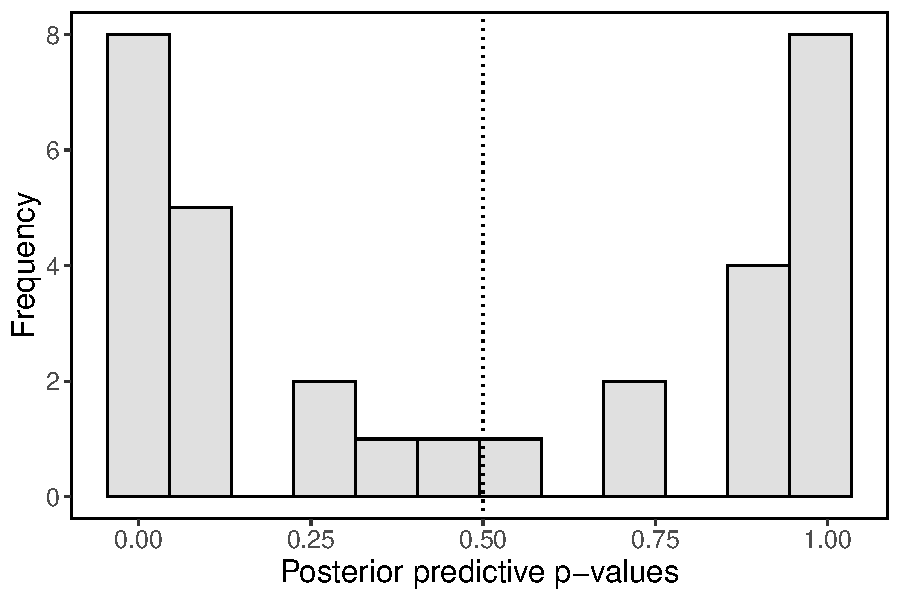
\includegraphics{Bayesian_GLMs_files/figure-latex/ch6-nb-ppcplot-1} 

}

\caption{\textbf{Frequency histogram of the posterior predictive p-values for the Bayesian negative binomial GLM with informative priors to predict coral biodiversity. The vertical dotted line indicates 0.5.}}\label{fig:ch6-nb-ppcplot}
\end{figure}

The frequency histogram of posterior predictive p-values in Fig. \ref{fig:ch6-nb-ppcplot} shows that most values are close to zero or 1, with few close to 0.5, indicating the model check has not been satisfied. We will proceed with further model checks.

\hypertarget{nbglm-cv}{%
\subsubsection{Cross-validation model checking}\label{nbglm-cv}}

We use leave-one-out cross validation to examine how well the model is able to generalise to new data. To ensure there are no potential numerical problems in estimating CPO or PIT for a given model, we first run the following check:

\texttt{sum(I01.pred\$cpo\$failure)}

0

An outcome of zero indicates no problems with the computation of CPO or PIT.

A uniform distribution of PIT values indicates whether the predictive distributions match the data (see the R script associated with this chapter).



\begin{figure}

{\centering 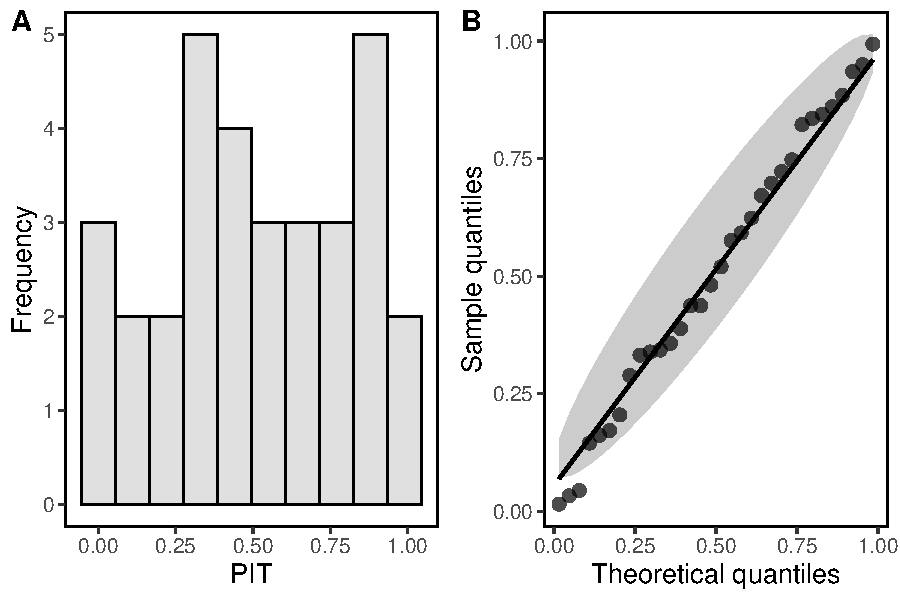
\includegraphics{Bayesian_GLMs_files/figure-latex/ch6-PIT-1} 

}

\caption{\textbf{A. Frequency histogram; B. Uniform Q-Q plot with confidence bands (shaded gray), for cross-validated PIT values for the Bayesian negative binomial GLM with informative priors.}}\label{fig:ch6-PIT}
\end{figure}

The frequency histogram of PIT values in Fig. \ref{fig:ch6-PIT}A shows that the distribution is broadly uniform. This conclusion is supported by the Q-Q plot (Fig. \ref{fig:ch6-PIT}B), which shows that the PIT values match a uniform distribution.

\hypertarget{nbglm-resids}{%
\subsubsection{Bayesian residuals analysis}\label{nbglm-resids}}

The homogeneity of residual variance can be assessed visually by plotting model residual variance against fitted values as well as each variable in the model (see the R script associated with this chapter).



\begin{figure}

{\centering 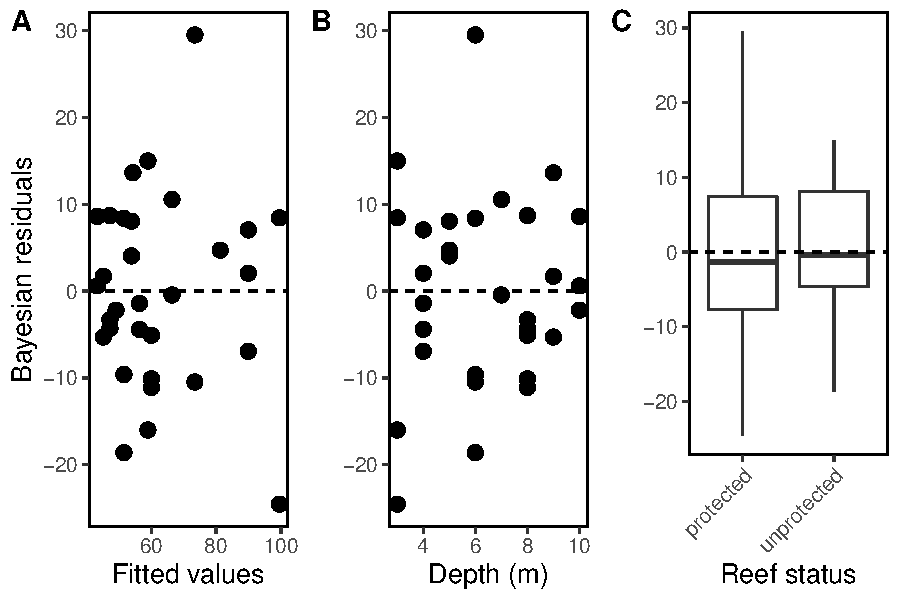
\includegraphics{Bayesian_GLMs_files/figure-latex/ch6-nb-resids-1} 

}

\caption{\textbf{Bayesian residuals plotted against: A. fitted values; B. water depth; and C. reef protected status, to assess homogeneity of residual variance.}}\label{fig:ch6-nb-resids}
\end{figure}

Ideally, the distribution of residuals around zero should be random along the horizontal axis, and in the case of a categorical variable (Fig. \ref{fig:ch6-nb-resids}C) the median of a boxplot of residuals should be approximately zero. For Figs. \ref{fig:ch6-nb-resids}A-C the pattern of residuals is acceptable.

\hypertarget{nb-sens}{%
\subsubsection{Prior sensitivity analysis}\label{nb-sens}}

A final model check is to examine prior distributions through a sensitivity analysis that involves systematically changing prior distributions and examining the magnitude of outcome for the posterior distribution.

In Chapters \ref{gen-model} and \ref{pois-glm} we investigated prior sensitivity by increasing and decreasing priors on the fixed effects by 20\% and examined the outcome for the posterior mean (see the R script associated with these chapters). In the case of the coral reef data, plots of the posterior distributions for the model fixed effects similarly indicate that the posterior distributions are robust to changes in the priors placed on them (analysis not shown).

\hypertarget{nb-checkconc}{%
\subsubsection{Conclusions from model checks}\label{nb-checkconc}}

The Poisson GLM with informative priors showed a comparable goodness-of-fit to that of the model with default priors. An analysis of model dispersion identified a problem with overdispersion, though this problem was corrected by fitting a negative binomial GLM. Leave-one-out cross validation indicated that the predictive distributions matched the data well and residuals plots failed to highlight any systematic problems with model fit. Prior sensitivity analysis demonstrated that the model was robust to changes in prior distributions of fixed effects. Overall, then, the Bayesian negative binomial GLM with informative priors provides a reasonable representation of the data.

\hypertarget{nb-present}{%
\subsection{Interpret and present model output}\label{nb-present}}

Specification of the Bayesian negative binomial GLM using mathematical notation takes the form:

\(Species_{i}\) \textasciitilde{} \(NegBin(\mu_{i}, k)\)

\emph{E}(\(Species_{i}\)) = \(\mu_i\) and var(\(Species_{i}\)) = \(\mu_i\) + (\(\mu_i^2 / k\))

\emph{log}\(\mu_i\) = \(\eta_i\)

\(\eta_i\) = \(\beta_1\) + \(\beta_2\) x \(Depth_{i}\) + \(\beta_3\) x \(Status_{i}\) + \(\beta_4\) x \(Depth_{i} : Status_{i}\)

Where \(Species_{i}\) is the number of scleractinian coral species at sample site \emph{i} assuming a negative binomial distribution with mean \(\mu_i\) and variance \(\mu_i\) + (\(\mu_i^2 / k\)). The parameter \emph{k} is the dispersion parameter and deals with the extra variance in the data. \(Depth_{i}\) is water depth for sample site \emph{i}, and \(Status_{i}\) is the protected status of the reef at sample site \emph{i.} Note that the model has a log link function

The numerical output of the model is:

\begin{verbatim}
                         mean   sd 0.025quant 0.975quant
(Intercept)              4.90 0.11       4.69       5.12
depth                   -0.10 0.02      -0.13      -0.07
statusunprotected       -0.69 0.15      -0.98      -0.41
depth:statusunprotected  0.06 0.02       0.01       0.10
\end{verbatim}

These results can be more formally presented in the following way:

Table 6.2: \textbf{Posterior mean estimates for number of hard coral species at sites in the Sulu Sea as a function of water depth (m), protected status, and their interaction, modelled using a negative binomial GLM fitted with INLA. CrI are the Bayesian 95\% credible intervals.}

\begin{longtable}[]{@{}lccc@{}}
\toprule
Model parameter & Posterior mean & Lower 95\% CrI & Upper 95\% CrI \\
\midrule
\endhead
Intercept & 4.90 & 4.69 & 5.12 \\
Depth & -0.10 & -0.13 & -0.07 \\
Status (unprotected) & -0.69 & -0.98 & -0.41 \\
Depth x Status & 0.06 & 0.01 & 0.10 \\
\bottomrule
\end{longtable}

These results (Table 6.2) show a statistically important negative effect of depth and reef protected status on coral biodiversity as well as an interaction between covariates.

\hypertarget{visualise-the-results-2}{%
\subsection{Visualise the results}\label{visualise-the-results-2}}

The negative binomial GLM can be visualised to assist with understanding the model outcomes. Coding for this plot is available in the R script associated with this chapter.



\begin{figure}
\centering
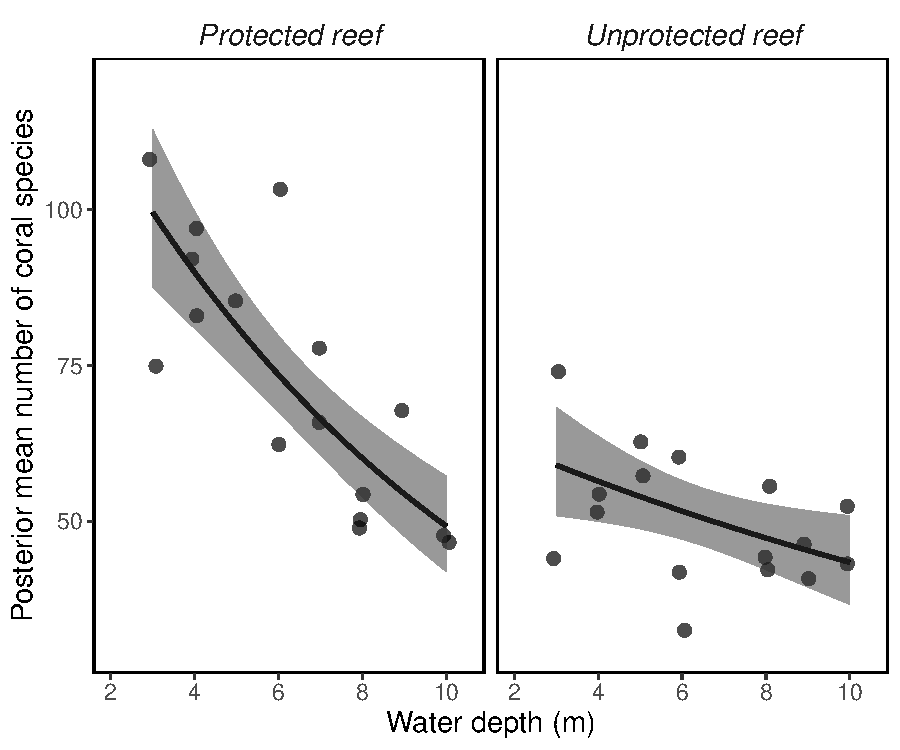
\includegraphics{Bayesian_GLMs_files/figure-latex/ch6-final-plot-1.pdf}
\caption{\label{fig:ch6-final-plot}\textbf{Posterior mean number of coral species from sampling sites in the Sulu Sea as a function of water depth (m) and protected status, modelled using a negative binomial GLM fitted with INLA. Shaded areas are Bayesian 95\% credible intervals. Black points are observed data for different sampling sites.}}
\end{figure}

The results of this statistical analysis can be summarised as follows:

\emph{A negative binomial GLM was fitted to data using Bayesian inference with INLA for the number of scleractinian coral species from 32 sampling 100 m\(^2\) sites in the Sulu Sea. In the best-fitting model, which included informative and weakly informative priors on fixed effects, there was a statistically important negative effect of water depth on number of coral species. There was also a statistically important effect of protected status, with fewer coral species in unprotected sites. Finally, there was an interaction between depth and protected status, with a steeper negative relationship between water depth and number of coral species at protected sites (Table 6.2), Fig. \ref{fig:ch6-final-plot}. The model was fitted using informative and weakly informative priors on the fixed effects, obtained from a separate study of coral biodiversity from the same biogeographic region.}

\hypertarget{conclusions-3}{%
\section{Conclusions}\label{conclusions-3}}

In this analysis we identified a problem with overdispersion in a Poisson GLM. Overdispersion in the Poisson model was treated as true overdispersion, with a GLM fitted with a negative binomial distribution, which successfully modelled the extra variance in the data. The goodness of fit of the negative binomial model, measured by the DIC, was also superior to the Poisson GLM

\hypertarget{bern-glm}{%
\chapter{Bayesian Bernoulli GLM}\label{bern-glm}}

A Bernoulli distribution is a discrete distribution for dealing with data with only two possible outcomes, such as success and failure or presence and absence. The Bernoulli GLM is for strictly binary data and is sometimes called a logistic GLM (or just ``logistic regression''). In ecology, a Bernoulli GLM is a particularly useful statistical tool for modelling presence/absence data.

\hypertarget{bern-cc}{%
\section{Common cuckoo parasitism of great reed warbler nests}\label{bern-cc}}

The common cuckoo (\emph{Cuculus canorus}) is an avian brood parasite, laying its eggs in the nests of its host species, which subsequently rear the parasitic cuckoo chick to independence. The common cuckoo exploits a range of hosts, with each individual female cuckoo a host specialist, exploiting a single or small group of host species. An important host is the great reed warbler (\emph{Acrocephalus arundinaceus}), which nests in reedbeds associated with waterbodies across lowland Europe. Because brood parasitism imposes a severe fitness cost on hosts, hosts have evolved defensive adaptations, including cryptic nesting behaviour as well as aggression towards cuckoos; reed warblers are capable of killing cuckoos that attempt to lay in their nests \citep{_ulc_2020}.

Here we fit a Bernoulli GLM to data on the occurrence of cuckoo parasitism in reed warbler nests in reedbeds associated with a marshland area in the South Moravian region of the Czech Republic. Data were collected for 18 nests during a single breeding season. Each nest was monitored over the entire breeding season, with a record made of whether or not the nest suffered cuckoo brood parasitism. Data were also collected for each nest on the distance to the nearest tree, which serve as vantage points for female cuckoos to observe the location of reed warbler nests. An additional habitat variable measured was the distance of each nest to open water, which provides a measure of how inaccessible a nest was in a given reedbed. Finally, the aggressive response of each pair of reed warblers to a dummy cuckoo placed 1 m from their nest was measured, with the response scored as either a low-level aggressive response (no reaction or distress calling) or high-level aggression (mobbing and attacking).

In addition to these data, a set of pilot data, comprising just 7 records, were collected in the year preceding the main study using identical methods. These data were used to assign priors to the main model.

\emph{\textbf{Import data}}

Data for cuckoo parasitism are saved in a comma-separated values (CSV) file \texttt{cuckoo.csv} and are imported into a dataframe in R using:

\texttt{cc\ \textless{}-\ read\_csv("cuckoo.csv")}

Start by inspecting the dataframe:

\texttt{str(cc)}

\begin{verbatim}
spec_tbl_df [18 x 5] (S3: spec_tbl_df/tbl_df/tbl/data.frame)
 $ nest   : num [1:18] 1 2 3 4 5 ...
 $ water  : num [1:18] 168 14 114 247 184 ...
 $ tree   : num [1:18] 54 73 12 55 21 ...
 $ aggress: chr [1:18] "low" "high" ...
 $ egg    : num [1:18] 1 0 1 0 1 ...
 - attr(*, "spec")=
  .. cols(
  ..   nest = col_double(),
  ..   water = col_double(),
  ..   tree = col_double(),
  ..   aggress = col_character(),
  ..   egg = col_double()
  .. )
\end{verbatim}

The dataframe comprises 18 observations of 5 variables. Each row in the dataframe represents a unique reed warbler nest (\texttt{nest}). There are two continuous ecological variables: \texttt{water} is the distance (in m) of each nest to open water, which represents the edge of the reedbed, and \texttt{tree} is the distance (in m) to the nearest tree that could act as a vantage point for female cuckoos to observe the reed warbler nest. There is a single categorical variable \texttt{aggress} with two levels; \texttt{high} and \texttt{low}, representing the level of the aggressive response of each pair of reed warblers to a dummy cuckoo. The binomial variable \texttt{egg}, is the response variable and indicates whether the nest escaped cuckoo parasitism (0) or received at least one cuckoo egg (1).

\hypertarget{bern-glm-steps}{%
\section{Steps in fitting a Bayesian GLM}\label{bern-glm-steps}}

We will following the 9 steps to fitting a Bayesian GLM, detailed in Section \ref{fit-steps}.

\emph{1. State the question}

\emph{2. Perform data exploration}

\emph{3. Select a statistical model}

\emph{4. Specify and justify a prior distribution on parameters}

\emph{5. Fit the model}

\emph{6. Obtain the posterior distribution}

\emph{7. Conduct model checks}

\emph{8. Interpret and present model output}

\emph{9. Visualise the results}

\hypertarget{cc-question}{%
\subsection{State the question}\label{cc-question}}

The aim of the study was to identify whether the three explanatory variables; \texttt{water}, \texttt{tree} and \texttt{aggress}, contributed to the probability that a great reed warbler nest would be parasitised by common cuckoos. The prediction was that probability of parasitism would be negatively associated with distance of a nest to open water and the nearest tree. A greater likelihood of parasitism was predicted in the case that the pair of nesting reed warblers showed a low-level aggressive response to a dummy cuckoo.

\hypertarget{cc-eda}{%
\subsection{Data exploration}\label{cc-eda}}

A data exploration is critical to identifying any potential problems or unusual patterns in the data. First check for missing data.

\texttt{colSums(is.na(cc))}

\begin{verbatim}
   nest   water    tree aggress     egg 
      0       0       0       0       0 
\end{verbatim}

There are no missing data.

\hypertarget{cc-outliers}{%
\subsubsection{Outliers}\label{cc-outliers}}

Outliers in the data can identified visually using Cleveland dotplots, R code is available in the R script associated with this chapter:



\begin{figure}

{\centering 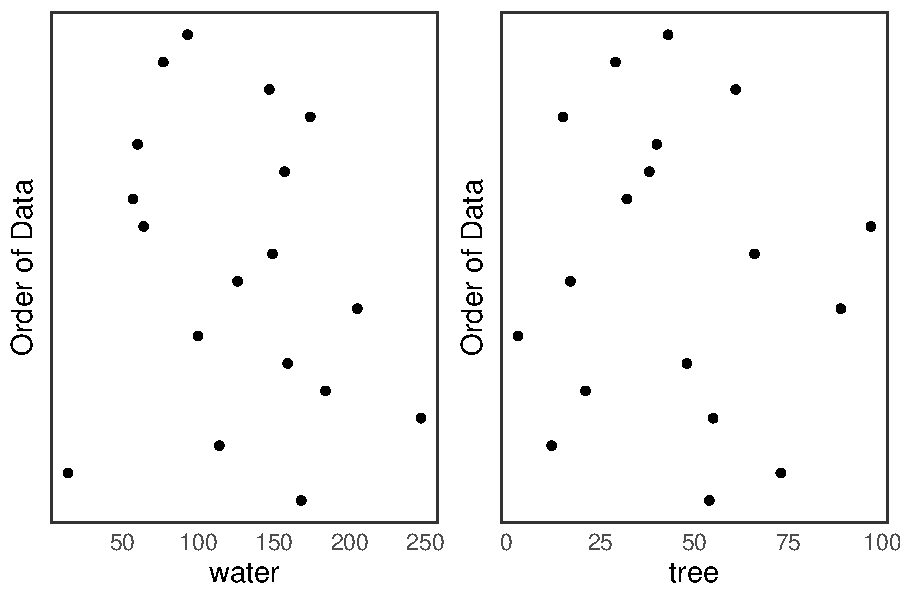
\includegraphics{Bayesian_GLMs_files/figure-latex/ch7-dotplot-1} 

}

\caption{\textbf{Dotplots of distance to open water (\texttt{water}) and a tree (\texttt{tree}) of reed warbler nests. Data are arranged by the order they appear in the dataframe.}}\label{fig:ch7-dotplot}
\end{figure}

There are no obvious outliers in the Fig. \ref{fig:ch7-dotplot}.

\hypertarget{bern-dist}{%
\subsubsection{Distribution of the dependent variable}\label{bern-dist}}

The distribution of the dependent variable is binomial; 0s and 1s. We can examine the balance of the response variable:

\texttt{table(cc\$egg)}

\begin{verbatim}
 0  1 
 8 10 
\end{verbatim}

Which shows that a total of 8 reed warbler nests escaped parasitism, while 10 received at least 1 cuckoo egg.

\hypertarget{bern-balance}{%
\subsubsection{Balance of categorical variables}\label{bern-balance}}

The balance of the categorical variable \texttt{aggress} (the aggressive response of each pair of reed warblers to a dummy cuckoo) is:

\texttt{table(cc\$aggress)}

\begin{verbatim}
high  low 
   9    9 
\end{verbatim}

The balance of this variable is perfect.

\hypertarget{bern-collin}{%
\subsubsection{Multicollinearity among covariates}\label{bern-collin}}

If covariates in a model are correlated, then there is a risk that the model may produce unstable parameter estimates with inflated standard errors. We visualise the relationships among model covariates using the \texttt{ggpairs} command from the \texttt{GGally} library:

\texttt{cc\ \%\textgreater{}\%\ ggpairs(columns\ =\ c("water",\ "tree",\ "aggress"),\ ggplot2::aes(colour=aggress,\ alpha\ =\ 0.8))}



\begin{figure}

{\centering 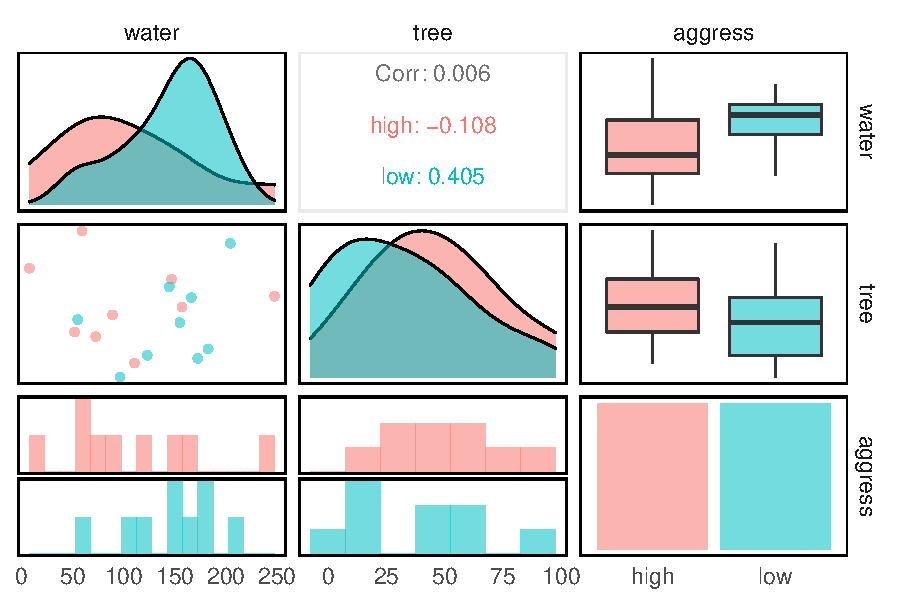
\includegraphics{Bayesian_GLMs_files/figure-latex/ch7-ggpairs-1} 

}

\caption{\textbf{Plot matrix of covariates showing frequency plots, boxplots, frequency histograms, and frequency polygons.}}\label{fig:ch7-ggpairs}
\end{figure}

The plot matrix in Fig. \ref{fig:ch7-ggpairs} indicates no evidence of collinearity.

\hypertarget{bern-zeros}{%
\subsubsection{Zeros in the response variable}\label{bern-zeros}}

The proportion of zeros in the response variable can be calculated with:

\texttt{round((sum(cc\$egg\ ==\ 0)\ /\ nrow(cc))*100,0)}

44

Unsurprisingly, the response variable contains a high proportion of zeros; 44\%. Given that \texttt{egg} is a binomial variable, this number of zeros is not problematic.

\hypertarget{bern-rels}{%
\subsubsection{Relationships among dependent and independent variables}\label{bern-rels}}

Visual inspection of the data using plots helps illustrate the nature of relationships among covariates (code for the plot is available in the R script associated with this chapter):



\begin{figure}

{\centering \includegraphics{Bayesian_GLMs_files/figure-latex/ch7-scatter-1} 

}

\caption{\textbf{Multipanel scatterplot of number of the probability of cuckoo parasitism against distance of nests to: A. open water and; B. a tree, for high and low aggression pairs of reed warblers.}}\label{fig:ch7-scatter}
\end{figure}

The plots in Fig. \ref{fig:ch7-scatter} suggest a greater risk of parasitism in the case of a low aggression response from reed warbler pairs. There is also some indication of a negative effect of tree distance and probability of parasitism. There is no clear effect of distance to open water or of an interaction among variables.

\hypertarget{bern-depend}{%
\subsubsection{Independence of response variable}\label{bern-depend}}

An assumption in fitting a GLM is that each observation is independent of all others. In the dataframe here, each row represents a separate nest guarded by a unique pair of reed warblers. This species is territorial and so, while pairs may have interacted on the edges of their territories, there was a minimum distance between nests and we will treat the data as independent, while recognising that some level of dependency is typical of much ecological data.

\hypertarget{bern-select}{%
\subsection{Selection of a statistical model}\label{bern-select}}

The aim of this study is to identify the contribution of three ecological and behavioural variables to the probability of cuckoo brood parasitism. The dependent variable is binomial with a single observation per `trial'; i.e.~a nest was either parasitised or not during the breeding season. Strictly then, this is not a binomial distribution but a Bernoulli distribution and will be modelled with a logit link function. The logit link function ensures that fitted model probabilities fall between 0 and 1.

\hypertarget{bern-prior-spec}{%
\subsection{Specification of priors}\label{bern-prior-spec}}

Informative priors for the model were based on data from a pilot study conducted in the year before the main study at the same location.

\hypertarget{pilot-study}{%
\subsubsection{Pilot study}\label{pilot-study}}

A small-scale trial in which just 7 great reed warbler nests were monitored for cuckoo parasitism was conducted in the year preceding the main trial. All reed warblers in the pilot and main study were ringed and none used in the pilot were subsequently monitored in the main study.

Table 7.1: \textbf{Pilot data to investigate predictors of cuckoo parasitism of great reed warbler nests. The association between the distance of nests to open water, the nearest tree, and reed warbler aggressive response to a dummy cuckoo were measured. The incidence of cuckoo brood parasitism of great reed warbler nests was monitored throughout the breeding season (mid-May to mid-July).}

\begin{longtable}[]{@{}ccccc@{}}
\toprule
Nest & Open water (m) & Tree (m) & Pair aggression & Cuckoo egg \\
\midrule
\endhead
a & 100 & 42 & high & 1 \\
b & 136 & 97 & high & 0 \\
c & 175 & 61 & low & 0 \\
d & 69 & 54 & low & 1 \\
e & 66 & 43 & high & 0 \\
f & 84 & 21 & low & 1 \\
g & 133 & 31 & low & 1 \\
\bottomrule
\end{longtable}

\emph{\textbf{Import pilot data}}

Pilot data are saved in the file \texttt{ccpilot.csv} and are imported into a dataframe in R using:

\texttt{ccpilot\ \textless{}-\ read\_csv("ccpilot.csv")}

Start by inspecting the dataframe:

\begin{verbatim}
spec_tbl_df [7 x 5] (S3: spec_tbl_df/tbl_df/tbl/data.frame)
 $ nest   : chr [1:7] "a" "b" "c" "d" ...
 $ water  : num [1:7] 100 136 175 69 66 84 133
 $ tree   : num [1:7] 42 97 61 54 43 21 31
 $ aggress: chr [1:7] "high" "high" "low" "low" ...
 $ egg    : num [1:7] 1 0 0 1 0 1 1
 - attr(*, "spec")=
  .. cols(
  ..   nest = col_character(),
  ..   water = col_double(),
  ..   tree = col_double(),
  ..   aggress = col_character(),
  ..   egg = col_double()
  .. )
\end{verbatim}

The dataframe comprises 7 observations of 5 variables, which are identical to those in the main study.

\hypertarget{model-pilot-data}{%
\subsubsection{Model pilot data}\label{model-pilot-data}}

We proceed by fitting a Bernoulli GLM to obtain parameter estimates to use as priors. We first formulate the model:

\texttt{f01\ \textless{}-\ egg\ \textasciitilde{}\ water\ +\ tree\ +\ aggress}

Then fit the model:

\texttt{P01\ \textless{}-\ inla(f01,\ family\ =\ "binomial",\ Ntrials\ =\ 1,\ data\ =\ ccpilot)}

The numerical output is obtained using:

\texttt{P01Betas\ \textless{}-\ P01\$summary.fixed{[},c("mean",\ "sd",\ "0.025quant",\ "0.975quant"){]}}

\texttt{round(P01Betas,\ digits\ =\ 2)}

\begin{verbatim}
             mean   sd 0.025quant 0.975quant
(Intercept)  1.68 1.88      -1.99       5.40
water       -0.01 0.02      -0.04       0.02
tree        -0.03 0.03      -0.10       0.03
aggresslow   1.83 1.60      -1.13       5.14
\end{verbatim}

The output provides parameter estimates that can be incorporated into our Bayesian model as informative priors for the full analysis.

\hypertarget{bern-priors-fixed}{%
\subsubsection{Priors on the fixed effects}\label{bern-priors-fixed}}

Non-informative (default) priors were put on the fixed effects for model \texttt{M01}, which were:

\(\beta intercept\) \textasciitilde{} \emph{N}(0, 0) (\(\tau\) = 0)

\(\beta water\) \textasciitilde{} \emph{N}(0, 1000) (\(\tau\) = 0.001)

\(\beta tree\) \textasciitilde{} \emph{N}(0, 1000) (\(\tau\) = 0.001)

\(\beta aggressionlow\) \textasciitilde{} \emph{N}(0, 1000) (\(\tau\) = 0.001)

The findings from the pilot data can be specified in model \texttt{I01} as informative priors on the fixed effects as:

\(\beta intercept\) \textasciitilde{} \emph{N}(1.68, 3.53) (\(\tau\) = 0.28)

\(\beta water\) \textasciitilde{} \emph{N}(-0.01, 0.0004) (\(\tau\) = 2500)

\(\beta tree\) \textasciitilde{} \emph{N}(-0.03, 0.0009) (\(\tau\) = 1111)

\(\beta aggressionlow\) \textasciitilde{} \emph{N}(1.83, 2.56) (\(\tau\) = 0.39)

\hypertarget{bern-fit-models}{%
\subsection{Fit the models}\label{bern-fit-models}}

We fit the Bayesian Bernoulli GLM using INLA with default priors (\texttt{M01}), and informative priors on the fixed effects (\texttt{I01}).

The model formulae (\texttt{f01}) is:

\texttt{f01\ \textless{}-\ egg\ \textasciitilde{}\ water\ +\ tree\ +\ aggress}

We fit the default model \texttt{M01}, specifying \texttt{control.compute\ =\ list(dic\ =\ TRUE)} to enable model comparison:

\texttt{M01\ \textless{}-\ inla(f01,\ family\ =\ "binomial",\ Ntrials\ =\ 1,\ data\ =\ cc,\ control.compute\ =\ list(dic\ =\ TRUE))}

Then fit the model with informative priors:

\texttt{I01\ \textless{}-\ inla(f01,\ family\ =\ "binomial",\ Ntrials\ =\ 1,\ data\ =\ cc,\ control.compute\ =\ list(dic\ =\ TRUE),\ control.fixed\ =\ list(mean.intercept\ =\ 1.68,\ prec.intercept\ =\ 1.88\^{}(-2),\ mean\ =\ list(water\ =\ -0.01,\ tree\ =\ -0.03,\ aggresslow\ =\ 1.83),\ prec\ =\ list(water\ =\ 0.02\^{}(-2),\ tree\ \ =\ 0.03\^{}(-2),\ aggresslow\ =\ 1.6\^{}(-2))))}

\hypertarget{bern-post-dist}{%
\subsection{Obtain the posterior distribution}\label{bern-post-dist}}

\hypertarget{model-with-default-priors-1}{%
\subsubsection{Model with default priors}\label{model-with-default-priors-1}}

Output for the fixed effects of M01 can be obtained with:

\texttt{M01Betas\ \textless{}-\ M01\$summary.fixed{[},c("mean",\ "sd",\ "0.025quant",\ \ "0.975quant"){]}}

\texttt{round(M01Betas,\ digits\ =\ 2)}

\begin{verbatim}
              mean   mode    sd 0.025quant 0.975quant
(Intercept) 195.84 164.09 45.04     131.41     301.86
water         0.37   0.27  0.18       0.08       0.79
tree         -5.41  -4.43  1.41      -8.74      -3.37
aggresslow   98.63  90.90 13.35      78.45     129.66
\end{verbatim}

This reports the posterior mean, standard deviation and 95\% credible intervals for the model intercept and covariates.

For the slope of the variable \texttt{water} the posterior mean is 0.37, lower 95\% credible interval 0.08 and upper 95\% credible interval 0.79. This result indicates that we can be 95\% certain that the posterior mean of the regression parameter for the slope of \texttt{water} falls between these credible intervals, which means \texttt{water} is statistically important in the model with uninformative priors.

We can similarly conclude that there is a statistically important negative effect of distance to the nearest tree and a positive effect of parental reed warbler aggressive response on the probability of cuckoo parasitism.

The posterior distributions of the fixed effects can be visualized using \texttt{ggplot2}. See the R script associated with this chapter.



\begin{figure}

{\centering \includegraphics{Bayesian_GLMs_files/figure-latex/ch7-M01-betas-1} 

}

\caption{\textbf{Posterior and prior distributions for fixed parameters of a Bayesian Bernoulli GLM to model the probability of common cuckoo brood parasitism of great reed warbler nests. The model is fitted with default (non-informative) priors. Distributions for: A. model intercept; B. slope for distance to open water; C. slope for distance to nearest tree; D. effect of parental reed warbler aggressive response. The solid black line is the posterior distribution, the solid gray line is the prior distribution, the gray shaded area encompasses the 95\% credible intervals, the vertical dashed line is the posterior mode of the parameter, the vertical dotted line indicates zero. For parameters where zero (indicated by dotted line) falls outside the range of the 95\% credible intervals (gray shaded area), the parameter is statistically important.}}\label{fig:ch7-M01-betas}
\end{figure}

Figure \ref{fig:ch7-M01-betas} provides a visual summary of the model fixed effects, and indicates that for model M01 the betas are all statistically important. Note that the posterior distributions are asymmetric; this feature reflects a problem with the model that is addressed in Section \ref{bern-freq-comp}.

\hypertarget{bern-inf-priors}{%
\subsubsection{Model with informative priors}\label{bern-inf-priors}}

The output for the model with informative priors is obtained with:

\texttt{I01Betas\ \textless{}-\ I01\$summary.fixed{[},c("mean",\ "mode",\ "sd",\ "0.025quant",\ "0.975quant"){]}}
\texttt{round(I01Betas,\ digits\ =\ 2)}

\begin{verbatim}
             mean  mode   sd 0.025quant 0.975quant
(Intercept)  2.90  2.85 1.23       0.54       5.37
water       -0.01 -0.01 0.01      -0.03       0.01
tree        -0.06 -0.06 0.02      -0.11      -0.03
aggresslow   2.47  2.37 1.08       0.44       4.69
\end{verbatim}

The results for the informative model differ quantitatively and quantitatively from the model with default priors. Parameter estimates are strikingly different and distance to open water is not statistically important in the model.

We can calculate the posterior odds ratio of model parameters by exponentiating model coefficients. For \texttt{tree} the odds ratio is \emph{exp}(-0.063) = 0.94; thus we can predict that there is an average 6\% (= 1 - 0.94) decrease in the odds of a reed warbler nest receiving a cuckoo egg for each 1 m increase in distance from the nearest tree, with 95\% certainty that this estimate falls between 2-10\%. The prior odds ratio for \texttt{tree} is 3\%.

The posterior distributions can be visualized with \texttt{ggplot2}: see the R script associated with this chapter.



\begin{figure}

{\centering \includegraphics{Bayesian_GLMs_files/figure-latex/ch7-I01-betas-1} 

}

\caption{\textbf{Posterior and prior distributions for fixed parameters of a Bayesian Bernoulli GLM to model the probability of common cuckoo brood parasitism of great reed warbler nests fitted with informative priors. Distributions for: A. model intercept; B. slope for distance to open water; C. slope for distance to nearest tree; D. effect of parental reed warbler aggressive response. The solid black line is the posterior distribution, the solid gray line is the prior distribution, the gray shaded area encompasses the 95\% credible intervals, the vertical dashed line is the posterior mode of the parameter, the vertical dotted line indicates zero. For parameters where zero (indicated by dotted line) falls outside the range of the 95\% credible intervals (gray shaded area), the parameter is statistically important.}}\label{fig:ch7-I01-betas}
\end{figure}

Figure \ref{fig:ch7-I01-betas} illustrates that for model I01 the betas for model intercept, tree and aggression all differ from zero and are statistically important. In contrast, the slope for water does not differ from zero. Note also that the posterior distributions are normally distributed, in contrast to those for the model with non-informative priors (Fig. \ref{fig:ch7-M01-betas}).

\hypertarget{bern-prior-comp}{%
\subsubsection{Comparison of models with uninformative and informative priors}\label{bern-prior-comp}}

We can compare the results of the Bernoulli GLMs with uninformative and informative priors using the DIC:

First extract DICs:

\texttt{InfDIC\ \textless{}-\ c(M01\$dic\$dic,\ I01\$dic\$dic)}

Add weighting:

\texttt{InfDIC.weights\ \textless{}-\ aicw(InfDIC)}

Add names:

\texttt{rownames(InfDIC.weights)\ \textless{}-\ c("default","informative")}

Print DICs:

\texttt{dprint.inf\ \textless{}-\ print\ (InfDIC.weights,\ abbrev.names\ =\ FALSE)}

Order DICs by fit:

\texttt{round(dprint.inf{[}order(dprint.inf\$fit),{]},2)}

\begin{verbatim}
                 fit    delta            w
default     40.83404 27.71673 9.580493e-07
informative 13.11730  0.00000 9.999990e-01
\end{verbatim}

\begin{verbatim}
              fit delta w
informative 13.12  0.00 1
default     40.83 27.72 0
\end{verbatim}

The DIC score for the informative model is substantially lower than that for the model with uninformative priors. Model weight (\(\omega\)) is the probability that a given model is the best model (based on DIC), given the data and the alternative models. In this case the model with informative priors is the most probable of the two.

\hypertarget{bern-freq-comp}{%
\subsubsection{Comparison with frequentist Bernoulli GLM}\label{bern-freq-comp}}

We can compare the results of the Bayesian Poisson GLMs with the same model fitted in a frequentist setting. Execution of the model in a frequentist framework can be performed with:

\texttt{Freq\ \textless{}-\ glm(egg\ \textasciitilde{}\ water\ +\ tree\ +\ aggress,\ family\ =\ binomial\ (link\ =\ "logit"),\ data\ =\ cc)}

\texttt{round(summary(Freq)\$coef{[},1:4{]},2)}

\begin{verbatim}
            Estimate Std. Error z value Pr(>|z|)
(Intercept)   170.01  176237.31       0        1
water           0.35    1337.61       0        1
tree           -5.24    4829.82       0        1
aggresslow     75.75  126040.27       0        1
\end{verbatim}

\texttt{Warning:}\strut \\
\texttt{glm.fit:\ algorithm\ did\ not\ converge}

\texttt{Warning:}\strut \\
\texttt{glm.fit:\ fitted\ probabilities\ numerically\ 0\ or\ 1\ occurred}

Note the warning messages. These warnings arise because some of the fitted probabilities are extremely close to zero or one. Note that the standard errors are unrealistically large, making model estimates unreliable.

We can compare this output with the results for the two Bayesian models:

Table 7.2: \textbf{Comparison of model parameters for frequentist, Bayesian model with non-informative and informative priors of Bernoulli GLM model to investigate common cuckoo brood parasitism of great reed warblers in South Moravia.}

\begin{longtable}[]{@{}lcccc@{}}
\toprule
Model & Intercept & water & tree & aggression \\
\midrule
\endhead
Frequentist & 185(480365) & 0.39(3689) & -5.71(13125) & 82.4(346541) \\
Bayesian (default) & 196(45.0) & 0.37(0.18) & -5.41(1.41) & 98.6(13.3) \\
Bayesian (inform) & 2.90(1.23) & -0.01(0.01) & -0.06(0.02) & 2.47(1.08) \\
\bottomrule
\end{longtable}

Parameter estimates for the frequentist and Bayesian model with non-informative priors are somewhat similar, though the variances for model parameters for each are decidedly different. Results for the Bayesian model with informative priors are starkly different to the results for the other two models.

How should we view these contrasting results? The failure of the frequentist model to converge highlights a problem with the model that is not resolved by fitting a Bayesian model with default priors. It is noteworthy that putting informative priors on model parameters had the effect of stabilising estimates, and the inclusion of at least weakly informative priors in this situation is a recommended solution to this problem \citep{Gelman_2008}. As a consequence, the model with informative priors is the one on which we can place greater reliance and with which we will conduct model checks.

\hypertarget{conduct-model-checks-3}{%
\subsection{Conduct model checks}\label{conduct-model-checks-3}}

After model fitting and obtaining the posterior distributions, a next step is validation of the model through model checks. However, model validation of Bernoulli GLMs is rather difficult, given the binary nature of the response variable.

\hypertarget{bern-dic}{%
\subsubsection{Model selection using the Deviance Information Criterion (DIC)}\label{bern-dic}}

We can perform a simple model selection by removing model parameters and comparing models using the DIC. Though also consider that model selection is not an obligatory step, and leaving the model as originally formulated is perfectly acceptable; see a fuller discussion of model selection in \citep{Smith_etal_2020}. We start by formulating a set of alternative models:

\texttt{f01\ \textless{}-\ egg\ \textasciitilde{}\ water\ +\ tree\ +\ aggress}

\texttt{f02\ \textless{}-\ egg\ \textasciitilde{}\ water\ +\ tree}

\texttt{f03\ \textless{}-\ egg\ \textasciitilde{}\ water\ +\ aggress}

\texttt{f04\ \textless{}-\ egg\ \textasciitilde{}\ tree\ +\ aggress}

To use DIC we must re-run the model with informative priors and specify \texttt{control.compute\ =\ list(dic\ =\ TRUE)}. See the R script associated with this chapter.

Compare models with the DIC:

\begin{verbatim}
                       I01dic
water + tree + aggress   13.1
water + tree             15.9
water + aggress          23.3
tree + aggress           12.5
\end{verbatim}

The full model (\texttt{water} + \texttt{tree} + \texttt{aggress}) and the model with water dropped (\texttt{tree} + \texttt{aggress}) provide the best fit, but the two are essentially indistinguishable. In this case we will choose the simpler of the two (i.e.~\texttt{tree} + \texttt{aggress}).

We can repeat this process to further refine the model (see R script associated with this chapter), though this process demonstrates that dropping further variables does not improve model fit based on the DIC.

\hypertarget{bern-ppc}{%
\subsubsection{Posterior predictive checks}\label{bern-ppc}}

Posterior predictive checks can be used to assess whether a model generates realistic predictions by drawing simulated estimates from the joint posterior predictive distribution and comparing them with observed data with a posterior predictive p-value. In the case of a Bernoulli distribution, this is a problematic since the outcome can take values only of 0 or 1.

Here we compare the predicted outcome for each reed warbler nest in terms of whether they were parasitised by a cuckoo egg or not, with observed parasitism. See the R script associated with this chapter for estimating and plotting the posterior predictive p-values for the model.



\begin{figure}

{\centering \includegraphics{Bayesian_GLMs_files/figure-latex/ch7-ppcplot-1} 

}

\caption{\textbf{Plot of the posterior predictive p-values (ppp) and observed occurrence of cuckoo eggs in reed warbler nests for the Bayesian Bernoulli GLM with informative priors for each nest in the study. Black points are observed outcomes and gray points are simulated model predictions.}}\label{fig:ch7-ppcplot}
\end{figure}

The plot of posterior predictive p-values and observed cuckoo parasitism of nests in Fig. \ref{fig:ch7-ppcplot} shows that simulated and observed nest outcomes correspond in every case.

\hypertarget{bern-resids}{%
\subsubsection{Bayesian residuals analysis}\label{bern-resids}}

The homogeneity of residual variance can be assessed visually by plotting model residual variance against fitted values as well as each variable in the model (see the R script associated with this chapter).



\begin{figure}

{\centering \includegraphics{Bayesian_GLMs_files/figure-latex/ch7-bern-resids-1} 

}

\caption{\textbf{Bayesian residuals plotted against: A. fitted values; B. distance to nearest tree; and C. parental aggression, to assess homogeneity of residual variance.}}\label{fig:ch7-bern-resids}
\end{figure}

Residuals plots for Bernoulli models are difficult to interpret, particularly if the number of observations is low (as in this case). Ideally, the distribution of residuals around zero should be random along the horizontal axis and in the case of a categorical variables (such as Fig. \ref{fig:ch7-bern-resids}C) the median of a boxplot of residuals should be approximately zero. For Figs. \ref{fig:ch7-bern-resids}A-C the pattern of residuals is not perfect, but appears acceptable.

\hypertarget{bern-sens}{%
\subsubsection{Prior sensitivity analysis}\label{bern-sens}}

A sensitivity analysis involves systematically changing prior distributions and examining the magnitude of outcome for the posterior distribution.

We investigated prior sensitivity by increasing and decreasing priors on the fixed effects by 20\% and examined the outcome for the posterior mean (see the R script associated with this chapter the full analysis).

Results for model with informative priors:

\begin{verbatim}
##              mean   sd 0.025quant 0.975quant
## (Intercept)  2.27 1.03       0.32       4.34
## tree        -0.07 0.02      -0.11      -0.03
## aggresslow   2.11 1.01       0.21       4.17
\end{verbatim}

Results for model with informative priors increased by 20\%:

\begin{verbatim}
##              mean   sd 0.025quant 0.975quant
## (Intercept)  2.83 1.18       0.61       5.23
## tree        -0.08 0.02      -0.13      -0.04
## aggresslow   2.38 1.14       0.25       4.73
\end{verbatim}

Results for model with informative priors decreased by 20\%:

\begin{verbatim}
##              mean   sd 0.025quant 0.975quant
## (Intercept)  1.77 0.88       0.09       3.52
## tree        -0.05 0.02      -0.09      -0.02
## aggresslow   1.83 0.87       0.17       3.59
\end{verbatim}

These results can be more formally presented in a table:

Table 7.3: \textbf{Sensitivity analysis for a 20\% increase and decrease in informative priors on fixed effects and the \% change in the posterior mean.}

\begin{longtable}[]{@{}lccccc@{}}
\toprule
Parameter & \% prior & Mean & 0.025CI & 0.975CI & \% posterior \\
\midrule
\endhead
& +20 & 2.83 & 0.61 & 5.23 & +24 \\
Intercept & 0 & 2.27 & 0.32 & 4.34 & 0 \\
& -20 & 1.77 & 0.09 & 3.52 & -22 \\
& & & & & \\
& +20 & -0.083 & -0.133 & -0.038 & +22 \\
tree & 0 & -0.068 & -0.110 & -0.030 & 0 \\
& -20 & -0.054 & -0.088 & -0.023 & -21 \\
& & & & & \\
& +20 & 2.38 & 0.25 & 4.73 & +13 \\
aggress & 0 & 2.11 & 0.21 & 4.17 & 0 \\
& -20 & 1.83 & 0.17 & 3.59 & -13 \\
\bottomrule
\end{longtable}

The results of the prior sensitivity analysis (Table 7.3) show that increases or decreases of 20\% in prior means result in equivalent or slightly lesser changes to the posterior distribution.

\hypertarget{bern-checkconc}{%
\subsubsection{Conclusions from model checks}\label{bern-checkconc}}

Model checks on Bernoulli GLMs are less straightforward than those for other distributions. However, the GLM with informative priors showed a substantially better goodness-of-fit than the model with default priors, which was a consequence of the priors serving to stabilise estimates. Posterior predictive checks confirmed that the model predictive distributions matched the data. Residual analysis failed to highlight any systematic problems with model fit. Prior sensitivity analysis demonstrated that the model was sensitive to changes in prior distributions of fixed effects, though in proportion to the changes to priors. Overall, then, the Bayesian Bernoulli GLM with informative priors appears to provides a reasonable representation of the data.

\hypertarget{bern-present}{%
\subsection{Interpret and present model output}\label{bern-present}}

Specification of the Bayesian Bernoulli GLM takes the form:

\(Egg_{i}\) \textasciitilde{} \(Binomial(\pi_{i}, n_{i})\)

\emph{E}(\(Egg_{i}\)) = \(n_i\) x \(\pi_{i}\) and var(\(Egg_{i}\)) = \(n_i\) x \(\pi_{i}\) x \((1 - \pi_{i})\)

\emph{logit} \(\pi_i\) = \(\eta_{i}\)

\(\eta_i\) = \(\beta_1\) + \(\beta_2\) x \(tree_{i}\) + \(\beta_3\) x \(aggression_{i}\)

Where \(Egg_{i}\) is the probability of nest \emph{i} being parasitised with a cuckoo egg, which is assumed to follow a binomial distribution with an expected probability (\emph{E}) of parasitism of mean \(n_i\) x \(\pi_{i}\) and variance \(n_i\) x \(\pi_{i}\) x \((1 - \pi_{i})\), with a logit link function. The logit function ensures the fitted probability of brood parasitism falls between 0 and 1. The model contains a linear effect for distance of nest \emph{i} to the nearest tree (\(tree_{i}\)), while \(aggression_{i}\) is a categorical covariate with two levels, corresponding with the aggressive response of parental great reed warblers to a cuckoo model, either low or high aggressive response.

The numerical output of the model is:

\begin{verbatim}
             mean   sd 0.025quant 0.975quant
(Intercept)  2.27 1.03       0.32       4.34
tree        -0.07 0.02      -0.11      -0.03
aggresslow   2.11 1.01       0.21       4.17
\end{verbatim}

These results can be more formally presented in the following way:

Table 7.4: \textbf{Posterior mean estimates for the probability of cuckoo eggs in the nests of great reed warblers at sites in South Moravia as a function of distance to the nearest tree (m) and parental reed warbler aggression, modelled using a Bernoulli GLM fitted with INLA. CrI are the Bayesian 95\% credible intervals.}

\begin{longtable}[]{@{}lccc@{}}
\toprule
Model parameter & Posterior mean & Lower 95\% CrI & Upper 95\% CrI \\
\midrule
\endhead
Intercept & 2.27 & 0.32 & 4.34 \\
Tree & -0.07 & -0.11 & -0.03 \\
Aggression (low) & 2.11 & 0.21 & 4.17 \\
\bottomrule
\end{longtable}

These results (Table 7.4) show a statistically important negative effect of distance to the nearest tree and parental aggression on the probability of brood parasitism of great reed warblers by common cuckoos.

\hypertarget{visualise-the-results-3}{%
\subsection{Visualise the results}\label{visualise-the-results-3}}

The outcome of the Bayesian Bernoulli GLM can be visualised to better appreciate the results. Coding for the figure is available in the R script associated with this chapter.



\begin{figure}
\centering
\includegraphics{Bayesian_GLMs_files/figure-latex/ch7-final-plot-1.pdf}
\caption{\label{fig:ch7-final-plot}\textbf{Posterior mean probability of brood parasitism of great reed warbler nests by the common cuckoo in South Moravia, Czech Republic as a function of distance to the nearest tree (m) and parental reed warbler aggression, modelled using a Bernoulli GLM fitted with INLA. Shaded areas are Bayesian 95\% credible intervals. Black points are observed data for different reed warbler nests.}}
\end{figure}

The results of this statistical analysis can be summarised as follows:

\emph{A Bayesian Bernoulli GLM was fitted to data on brood parasitism by the common cuckoo of 18 great reed warbler nests in South Moravia, Czech Republic. In the best-fitting model, which included informative priors on fixed effects derived from a pilot study, there was a statistically important negative effect of distance of nests to the nearest tree on probability of parasitism. There was also a statistically important effect of parental reed warbler aggression to a cuckoo model, with a lower probability of cuckoo brood parasitism associated with more aggressive reed warbler pairs (Table 7.4, Fig. \ref{fig:ch7-final-plot}).}

\hypertarget{conclusions-4}{%
\section{Conclusions}\label{conclusions-4}}

Informative priors proved efficient in stabilising model estimates as a consequence of fitted probabilities that were close to zero or one. A frequentist model fitted to the data failed to converge and generated unreliable parameter estimates, as did a Bayesian Bernoulli GLM with non-informative priors. The goodness-of-fit of the Bernoulli GLM with informative priors, measured by the DIC, was also superior to the same model with non-informative priors.

\hypertarget{gamma-glm}{%
\chapter{Bayesian gamma GLM}\label{gamma-glm}}

Gaussian GLMs assume that the response variable follows a normal statistical distribution. While we commonly model continuous response variables using a Gaussian GLM (Chapter 4), there are limitations to this approach. An assumption in fitting data to a Gaussian distribution is that variation around the mean is symmetric and that the data can be summarised by the arithmetic mean and standard deviation. However, the assumption that continuous biological data are necessarily drawn from a Gaussian distribution may not always be justified; some types of data are typically not symmetric. Another problem is that a normal statistical distribution can generate negative predictions. For some continuous data that ostensibly appear normally distributed, such as body size, negative values are clearly impossible.

A solution to modelling continuous data that deviate from normality is to transform data. A more satisfactory alternative is to use a distribution that better represents the data. One alternative is the gamma distribution. This distribution can be used to model continuous variables that are strictly positive (i.e.~no zeros or negative values) and positively skewed. The gamma distribution is appropriate for biological and ecological data such as body size, pollutant concentrations, or time intervals between (non-random) events.

\hypertarget{common-seal-dive-duration}{%
\section{Common seal dive duration}\label{common-seal-dive-duration}}

The common (harbour) seal (\emph{Phoca vitulina}) is a widespread phocid seal found throughout cold temperate and Arctic waters of the northern hemisphere. They are protected in the UK, which supports approximately 40\% of the world's population of this species. Common seals are generalist predators in coastal waters. They prey chiefly on fish, cephalopods and crustaceans and are capable of extended foraging dives lasting up to 30 minutes.

Data were collected on the maximum dive duration for 29 radio-tagged adult common seals from a population in the Moray Firth on the East coast of Scotland. All seals in the study were of known age, sex, total body length, and lean mass. Lean mass was calculated by deducting blubber mass (estimated from blubber thickness using ultrasound measurements) from total mass.

\emph{\textbf{Import data}}

The data are saved in a comma-separated values (CSV) file \texttt{seal.csv} and are imported into a dataframe in R using:

\texttt{seal\ \textless{}-\ read\_csv(file\ =\ "seal.csv")}

Start by inspecting the dataframe:

\texttt{str(seal)}

\begin{verbatim}
spec_tbl_df [29 x 5] (S3: spec_tbl_df/tbl_df/tbl/data.frame)
 $ id       : chr [1:29] "A20" "A31" ...
 $ sex      : num [1:29] 1 1 2 1 2 ...
 $ age      : num [1:29] 8 10 10 10 7 ...
 $ lean_mass: num [1:29] 77 105 100 85 86 ...
 $ dive_dur : num [1:29] 816 1128 ...
 - attr(*, "spec")=
  .. cols(
  ..   id = col_character(),
  ..   sex = col_double(),
  ..   age = col_double(),
  ..   lean_mass = col_double(),
  ..   dive_dur = col_double()
  .. )
\end{verbatim}

The dataframe comprises 29 observations of 5 variables. Each row in the dataframe represents a different radio-tagged common seal. Each animal has a unique identification code (\texttt{id}). \texttt{Sex} is a factor; i.e.~a categorical variable, though note that it has been coded numerically in the dataframe (1 = male, 2 = female). Seal age (\texttt{age}) in years, lean mass (kg) (\texttt{lean\_mass}), and maximum dive duration (sec.) (\texttt{div\_dur}) are all continuous covariates. Maximum dive duration is the response variable that we will model.

\hypertarget{gamma-glm-steps}{%
\section{Steps in fitting a Bayesian GLM}\label{gamma-glm-steps}}

We will following the 9 steps to fitting a Bayesian GLM:

\emph{1. State the question}

\emph{2. Perform data exploration}

\emph{3. Select a statistical model}

\emph{4. Specify and justify a prior distribution on parameters}

\emph{5. Fit the model}

\emph{6. Obtain the posterior distribution}

\emph{7. Conduct model checks}

\emph{8. Interpret and present model output}

\emph{9. Visualise the results}

\hypertarget{seal-question}{%
\subsection{State the question}\label{seal-question}}

This study was designed to understand which variables predicted dive duration in common seals. Specifically, the aims of the study were to test whether common seal dive duration was predicted by: 1. lean body mass; 2. age; 3. sex. Based on previous research on elephant seals (\emph{Mirounga} spp.) and Weddell seals (\emph{Leptonychotes weddellii}), our predictions were that larger individuals would show greater maximum dive duration, as would younger individuals. A further prediction was that males would exhibit greater dive duration than females.

Consequently there are three specific predictions to test:

\begin{enumerate}
\def\labelenumi{\arabic{enumi}.}
\item
  A positive association between lean body mass and maximum dive duration.
\item
  A negative association between seal age and maximum dive duration.
\item
  An association between maximum dive duration and sex, with males showing a greater maximum dive duration than females.
\end{enumerate}

\hypertarget{gamma-eda}{%
\subsection{Data exploration}\label{gamma-eda}}

We start by conducting a data exploration to identify any potential problems with the data. First check for missing data.

\texttt{colSums(is.na(seal))}

\begin{verbatim}
       id       sex       age lean_mass  dive_dur 
        0         0         0         0         0 
\end{verbatim}

No missing data.

\hypertarget{outliers-2}{%
\subsubsection{Outliers}\label{outliers-2}}

Outliers in the data can identified visually using multi-panel Cleveland dotplots The code for this plot is available in the R script associated with this chapter.



\begin{figure}

{\centering \includegraphics{Bayesian_GLMs_files/figure-latex/ch8-dotplot-1} 

}

\caption{\textbf{Dotplots of seal age (years) lean mass (kg) and dive duration (sec.) of common seals. Data are arranged by the order they appear in the dataframe.}}\label{fig:ch8-dotplot}
\end{figure}

There are no obvious outliers in Fig. \ref{fig:ch8-dotplot}

\hypertarget{gamma-dist}{%
\subsubsection{Distribution of the dependent variable}\label{gamma-dist}}

The distribution of the dependent variable will inform selection of the appropriate statistical model to use. Here we visualise seal dive duration with a density plot using the \texttt{geom\_density()} function from the \texttt{ggplot2} package. The coding for this plot is available in the R script associated with this chapter.



\begin{figure}

{\centering \includegraphics{Bayesian_GLMs_files/figure-latex/ch8-freqdens-1} 

}

\caption{Density plot of common seal dive duration for 29 individuals.}\label{fig:ch8-freqdens}
\end{figure}

The density plot of the dependent variable (Fig. \ref{fig:ch8-freqdens}) shows a distribution with a pronounced positive skew.

\hypertarget{gamma-balance}{%
\subsubsection{Balance of categorical variables}\label{gamma-balance}}

Because sex has been coded numerically, we will re-assign it as a factor:

\texttt{seal\$fSex\ \textless{}-\ factor(seal\$sex)}

For clarity we can also reassign `1' as male and `2' as female:

\texttt{seal\$fSex\ \textless{}-\ fct\_recode(seal\$fSex,\ Male\ =\ "1",\ Female\ =\ "2")}

We then examine the balance of this variable:

\texttt{table(seal\$fSex)}

\begin{verbatim}
  Male Female 
    15     14 
\end{verbatim}

The balance of this categorical variable is acceptable.

\hypertarget{gamma-collin}{%
\subsubsection{Multicollinearity among covariates}\label{gamma-collin}}

Here we examine the relationships among model covariates using the \texttt{ggpairs()} function from the \texttt{GGally} library.

We first create an object comprising the variables of interest, then plot:

\texttt{seal\ \%\textgreater{}\%\ ggpairs(columns\ =\ c("fSex",\ "age",\ "lean\_mass"),\ ggplot2::aes(colour=fSex,\ alpha\ =\ 0.8))}



\begin{figure}

{\centering \includegraphics{Bayesian_GLMs_files/figure-latex/ch8-ggpairs-1} 

}

\caption{\textbf{Plot matrix of common seal dive duration (sec.) split by sex, showing frequency plots, boxplots, frequency histograms, and frequency polygons.}}\label{fig:ch8-ggpairs}
\end{figure}

The plot matrix in Fig. \ref{fig:ch8-ggpairs} indicates a weak correlation of age and lean mass for both sexes.

We will calculate a variance inflation factor (VIF) for each variable. The VIF is an estimate of the proportion of variance in one predictor explained by all the other predictors in the model. A VIF of 1 indicates no collinearity. VIF values above 1 indicate increasing degrees of collinearity. VIF values exceeding 3 are considered problematic.

The VIF for a model can be estimated using the \texttt{vif()} function from the \texttt{car} package:

\texttt{round(vif(gamma1\ \textless{}-\ glm(dive\_dur\ \textasciitilde{}\ lean\_mass\ +\ age\ +\ fSex,\ family\ =\ Gamma(link\ =\ log),\ data\ =\ seal)),2)}

\begin{verbatim}
lean_mass       age      fSex 
     1.90      1.88      1.10 
\end{verbatim}

The estimated VIFs are all \textless3, so we have no problem with multicollinearity.

\hypertarget{gamma-zeros}{%
\subsubsection{Zeros in the response variable}\label{gamma-zeros}}

The number of zeros in the response variable can be calculated with:

\texttt{sum(seal\$dive\_dur\ ==\ 0)}

0

There are no zeros in the response variable (and logically dive duration cannot be for zero seconds).

\hypertarget{gamma-rels}{%
\subsubsection{Relationships among dependent and independent variables}\label{gamma-rels}}

Visual inspection of the data can illustrate whether relationships are linear or non-linear and whether there are interactions between covariates. See the coding for these plots in the R script associated with this chapter.



\begin{figure}

{\centering \includegraphics{Bayesian_GLMs_files/figure-latex/ch8-scatter-1} 

}

\caption{\textbf{Multipanel scatterplot of common seal dive duration (secs.) against lean mass (kg) and age (years) for males and females, with a line of best fit plotted.}}\label{fig:ch8-scatter}
\end{figure}

The plot of the data in Fig. \ref{fig:ch8-scatter} does not suggest non-linear patterns in the data. Fitted lines for the relationship between dive duration and lean mass and age suggest positive relationships for both sexes, though we should also note that lean mass and age are weakly correlated. There is no clear evidence of an interaction of sex and lean mass or age. Given the patterns in these data, inclusion of an interaction term in a model is not justified.

\hypertarget{gamma-indep}{%
\subsubsection{Independence of response variable}\label{gamma-indep}}

A critical assumption for a GLM is that each observation in a dataset is independent of all others. For some data this assumption is difficult to confirm but can be reduced by careful sampling. Strictly randomly collected samples will tend to be independent.

For these data common seals were selected and tagged at random. The research was conducted by an experienced group of scientists with specialist knowledge of the species, a good understanding of statistics and ecological survey design, and clear research aims. In this case, we can assume that data were collected in a way to ensure their independence.

\hypertarget{gamma-select}{%
\subsection{Selection of a statistical model}\label{gamma-select}}

The response variable is strictly positive (no zeros, no negative values) and positively skewed. Rather than attempt to correct the non-normality and skewness in the data with a transformation and fit the model as a Gaussian GLM, an alternative approach is to model the data with a gamma distribution and a log link function. Three covariates will be included in the model as predictors of dive duration; lean mass (continuous), age (continuous) and sex (categorical, with two levels).

\hypertarget{gamma-prior-spec}{%
\subsection{Specification of priors}\label{gamma-prior-spec}}

There are no previous studies comparable to this one on common seals to provide priors and a pilot study was not conducted. However, there have been a number of studies on related species, particularly elephant seals (\emph{Mirounga} spp.) and Weddell seals (\emph{Leptonychotes weddellii}). Consequently, our prior distributions will be weakly informative with the predictions that larger and younger individuals will show a longer maximum dive duration, and males will show greater dive duration than females.

\hypertarget{gamma-priors-fixed}{%
\subsubsection{Priors on the fixed effects}\label{gamma-priors-fixed}}

Non-informative (default) priors were put on the fixed effects for model M01, which were:

\(\beta intercept\) \textasciitilde{} \emph{N}(0, 0) (\(\tau\) = 0)

\(\beta mass\) \textasciitilde{} \emph{N}(0, 1000) (\(\tau\) = 0.001)

\(\beta age\) \textasciitilde{} \emph{N}(0, 1000) (\(\tau\) = 0.001)

\(\beta fSex\) \textasciitilde{} \emph{N}(0, 1000) (\(\tau\) = 0.001)

Weakly informative priors based on previous studies were specified for model I01 as:

\(\beta intercept\) \textasciitilde{} \emph{N}(5, 0.25) (\(\tau\) = 0.04)

\(\beta mass\) \textasciitilde{} \emph{N}(0.01, 0.0025) (\(\tau\) = 400)

\(\beta age\) \textasciitilde{} \emph{N}(-0.01, 0.0025) (\(\tau\) = 400)

\(\beta fSex\) \textasciitilde{} \emph{N}(-0.1, 0.25) (\(\tau\) = 4)

We assumed a weak positive effect of lean body mass of 0.01, with \(\sigma\) = 0.05. For age we assumed the same values, but in this case the relationship was predicted to be negative. For the categorical variable sex, we assumed a weak negative effect of females in comparison with males, based on research on other seal species, of -0.1, with \(\sigma\) = 0.5. For the model intercept, we assumed a low positive value of 5 s (\(\sigma\) = 0.5).

\hypertarget{gamma-hyper}{%
\subsubsection{Priors on the hyperparameter}\label{gamma-hyper}}

The default hyperparameter is a diffuse gamma distribution:

precision \textasciitilde{} loggamma(1, 10) (\(\tau\) = 0.01)

For the model with informative priors we will use an informative prior on the hyperparameter.

We first obtain the precision parameter phi (\(\phi\)) from model \texttt{M01}:

\texttt{phi\ \textless{}-\ M01\$summary.hyperpar{[}"Precision\ parameter\ for\ the\ Gamma\ observations",\ "mean"{]}}

Internally, INLA uses \(\phi\) = \emph{exp}(\(\theta\)). So:

\texttt{round(log(phi),2)}

5.43

So, the informative prior on the hyperparameter is designated as 5.43 with a large variance (low precision) of 1000:

precision \textasciitilde{} loggamma(5.43, 1000) (\(\tau\) = 0.001)

\hypertarget{gamma-fit-model}{%
\subsection{Fit the model}\label{gamma-fit-model}}

We fit the two Bayesian gamma GLMs using INLA, one with default priors (\texttt{M01}) and the second with weakly informative priors on the fixed effects, and hyperparameter (\texttt{I01}).

Model M01 is fitted as:

\texttt{M01\ \textless{}-\ inla(dive\_dur\ \textasciitilde{}\ lean\_mass\ +\ age\ +\ fSex,\ family\ =\ "gamma",\ data\ =\ seal,\ control.compute\ =\ list(dic\ =\ TRUE))}

The model with informative priors is fitted as:

\texttt{I01\ \textless{}-\ inla(dive\_dur\ \textasciitilde{}\ lean\_mass\ +\ age\ +\ fSex,\ data\ =\ seal,\ family\ =\ "gamma",\ control.compute\ =\ list(dic\ =\ TRUE),\ control.family\ =\ list(hyper\ =\ list(prec\ =\ list(prior\ =\ "loggamma",\ param\ =\ c(5.43,\ 31.6\^{}(-2))))),\ control.fixed\ =\ list(mean.intercept\ =\ 5,\ prec.intercept\ =\ 5\^{}(-2),\ mean\ =\ list(lean\_mass\ =\ 0.01,\ age\ =\ -0.01,\ fSexFemale\ =\ -0.1),\ prec\ =\ list(lean\_mass\ =\ 0.05\^{}(-2),\ age\ =\ 0.05\^{}(-2),\ \ fSexFemale\ =\ 0.5\^{}(-2))))}

\hypertarget{gamma-post-dist}{%
\subsection{Obtain the posterior distribution}\label{gamma-post-dist}}

\hypertarget{gamma-def-priors}{%
\subsubsection{Model with default priors}\label{gamma-def-priors}}

Output for the fixed effects of M01 can be obtained with:

\texttt{M01Betas\ \textless{}-\ I01\$summary.fixed{[},c("mean",\ "sd",\ "0.025quant",\ "0.975quant"){]}}

\texttt{round(M01Betas,\ digits\ =\ 3)}

\begin{verbatim}
              mean    sd 0.025quant 0.975quant
(Intercept)  6.161 0.060      6.043      6.279
lean_mass    0.008 0.001      0.007      0.010
age         -0.002 0.008     -0.018      0.013
fSexFemale  -0.069 0.021     -0.111     -0.027
\end{verbatim}

This reports the posterior mean, standard deviation and 95\% credible intervals for the intercept and covariates.

For the model intercept and variables \texttt{lean\_mass} and \texttt{fSexFemale} we have lower and upper 95\% credible intervals that do not include zero. In the case of \texttt{lean\_mass} the effect is positive and for \texttt{fSexFemale} negative. The slope for the variable \texttt{age} does not differ from zero.

The posterior distributions can be visualized using \texttt{ggplot2.} The coding for this plot is available in the R script associated with this chapter.



\begin{figure}

{\centering \includegraphics{Bayesian_GLMs_files/figure-latex/ch8-M01-betas-1} 

}

\caption{\textbf{Posterior and prior distributions for fixed parameters of a Bayesian gamma GLM to model maximum dive duration of common seals. The model is fitted with default (non-informative) priors. Distributions for: A. model intercept; B. slope for lean mass; C. slope for age; D. slope for sex. The solid black line is the posterior distribution, the solid gray line is the prior distribution, the gray shaded area encompasses the 95\% credible intervals, the vertical dashed line is the posterior mean of the parameter, the vertical dotted line indicates zero. For parameters where zero (indicated by dotted line) falls outside the range of the 95\% credible intervals (gray shaded area), the parameter is statistically important.}}\label{fig:ch8-M01-betas}
\end{figure}

Figure \ref{fig:ch8-M01-betas} provides a visual summary of the fixed effects, for model \texttt{M01} showing the betas for the intercept, lean mass and sex are statistically important.

Code to plot the posterior distributions for the precision and dispersion of the model hyperparameter is available in the R script associated with this chapter.

\hypertarget{gamma-inf-priors}{%
\subsubsection{Model with informative priors}\label{gamma-inf-priors}}

We obtain the posterior distributions for the model:

\texttt{I01Betas\ \textless{}-\ I01\$summary.fixed{[},c("mean",\ "sd",\ "0.025quant",\ "0.975quant"){]}}

\texttt{round(I01Betas,\ digits\ =\ 3)}

\begin{verbatim}
              mean    sd 0.025quant 0.975quant
(Intercept)  6.161 0.060      6.043      6.279
lean_mass    0.008 0.001      0.007      0.010
age         -0.002 0.008     -0.018      0.013
fSexFemale  -0.069 0.021     -0.111     -0.027
\end{verbatim}

Like the default model, the model intercept and variables \texttt{lean\_mass} and \texttt{fSexFemale} have lower and upper 95\% credible intervals that do not include zero. In contrast, the slope for the effect of seal age does not differ from zero.



\begin{figure}

{\centering \includegraphics{Bayesian_GLMs_files/figure-latex/ch8-I01-betas-1} 

}

\caption{\textbf{Posterior and prior distributions for fixed parameters of a Bayesian gamma GLM to model maximum dive duration of common seals. The model is fitted with weakly informative priors. Distributions for: A. model intercept; B. slope for lean mass; C. slope for age; D. slope for sex. The solid black line is the posterior distribution, the solid gray line is the prior distribution, the gray shaded area encompasses the 95\% credible intervals, the vertical dashed line is the posterior mean of the parameter, the vertical dotted line indicates zero. For parameters where zero (indicated by dotted line) falls outside the range of the 95\% credible intervals (gray shaded area), the parameter is statistically important.}}\label{fig:ch8-I01-betas}
\end{figure}

Figure \ref{fig:ch8-I01-betas} illustrates that for model \texttt{I01} the betas for the intercept, lean mass and sex are statistically important. The figure also shows the distributions of the weakly informative priors, derived from previous research on elephant and Weddell seals.

Code to plot the posterior distributions for the precision and dispersion of the model hyperparameter is available in the R script associated with this chapter.

\hypertarget{gamma-prior-comp}{%
\subsubsection{Comparison of models with uninformative and informative priors}\label{gamma-prior-comp}}

The results for the Bayesian gamma GLM with non-informative priors and the same model fitted with informative priors can be compared using the DIC:

First extract DICs:

\texttt{InfDIC\ \textless{}-\ c(M01\$dic\$dic,\ I01\$dic\$dic)}

Add weighting:

\texttt{InfDIC.weights\ \textless{}-\ aicw(InfDIC)}

Add names:

\texttt{rownames(InfDIC.weights)\ \textless{}-\ c("default","informative")}

Print DICs:

\texttt{dprint.inf\ \textless{}-\ print\ (InfDIC.weights,\ abbrev.names\ =\ FALSE)}

Order DICs by fit:

\texttt{round(dprint.inf{[}order(dprint.inf\$fit),{]},2)}

\begin{verbatim}
                 fit    delta         w
default     324.8671 1.031999 0.3737881
informative 323.8351 0.000000 0.6262119
\end{verbatim}

\begin{verbatim}
               fit delta    w
informative 323.84  0.00 0.63
default     324.87  1.03 0.37
\end{verbatim}

The fit for the informative model is marginally better than that with uninformative priors and is more probable. The improvement in fit comes from the weakly informative priors on the fixed effects and hyperparameter.

\hypertarget{gamma-freq-comp}{%
\subsubsection{Comparison with frequentist gamma GLM}\label{gamma-freq-comp}}

We compare the results of the Bayesian gamma GLMs with the same model fitted in a frequentist setting. Execution of the model in a frequentist framework can be performed with:

\texttt{Freq\ \textless{}-\ glm(dive\_dur\ \textasciitilde{}\ lean\_mass\ +\ age\ +\ fSex,\ family\ =\ Gamma(link\ =\ log),\ data\ =\ seal)}

The results are obtained with:

\texttt{round(summary(Freq)\$coef{[},1:4{]},3)}

\begin{verbatim}
            Estimate Std. Error t value Pr(>|t|)
(Intercept)    6.160      0.070  88.307    0.000
lean_mass      0.008      0.001   8.138    0.000
age           -0.002      0.009  -0.223    0.825
fSexFemale    -0.069      0.024  -2.845    0.009
\end{verbatim}

We can estimate the dispersion parameter of the model:

\texttt{round(summary(Freq)\$dispersion,3)}

0.004

We can compare these with the results for the Bayesian models:

Table 8.1: \textbf{Comparison of model parameters for frequentist, Bayesian model with non-informative and informative priors of gamma GLM model to investigate maximum dive duration of common seals.}

\begin{longtable}[]{@{}lcccc@{}}
\toprule
Model & Intercept & lean mass & age & sex \\
\midrule
\endhead
Frequentist & 6.16(0.07) & 0.008(0.001) & 0.002(0.009) & 0.069(0.024) \\
Bayesian (default) & 6.16(0.06) & 0.008(0.001) & 0.002(0.008) & 0.069(0.021) \\
Bayesian (inform) & 6.16(0.06) & 0.008(0.001) & 0.002(0.008) & 0.069(0.021) \\
\bottomrule
\end{longtable}

Parameter estimates for the fixed effects for all the models are essentially identical.

\hypertarget{conduct-model-checks-4}{%
\subsection{Conduct model checks}\label{conduct-model-checks-4}}

\hypertarget{gamma-dic}{%
\subsubsection{Model selection using the Deviance Information Criterion (DIC)}\label{gamma-dic}}

We perform a simple model selection by removing model parameters and comparing models using the DIC for the Bayesian gamma GLM with weakly informative priors. Start by formulating alternative models:

\texttt{f01\ \textless{}-\ dive\_dur\ \textasciitilde{}\ lean\_mass\ +\ age\ +\ fSex}

\texttt{f02\ \textless{}-\ dive\_dur\ \textasciitilde{}\ lean\_mass\ +\ age}

\texttt{f03\ \textless{}-\ dive\_dur\ \textasciitilde{}\ lean\_mass\ +\ fSex}

\texttt{f04\ \textless{}-\ dive\_dur\ \textasciitilde{}\ age\ +\ fSex}

To use DIC we must re-run the model and specify its calculation using \texttt{control.compute}. See the R script associated with this chapter.

The results of model selection show:

\begin{verbatim}
                       I01dic
lean_mass + age + fSex  323.8
lean_mass + age         330.0
lean_mass + fSex        322.1
age + fSex              359.3
\end{verbatim}

The model comprising \texttt{lean\_mass} and \texttt{fSex} is the best fitting. We will conduct checks on a model with weakly informative priors and these parameters.

\hypertarget{gamma-ppc}{%
\subsubsection{Posterior predictive checks}\label{gamma-ppc}}

If the posterior predictive p-value is close to 0.5 it means simulated and observed data are similar, whereas if close to 1 it means the model prediction is too high and if close to zero, too low.

See the R script associated with this chapter for estimating and plotting the posterior predictive p-values for the model.



\begin{figure}

{\centering \includegraphics{Bayesian_GLMs_files/figure-latex/ch8-gamma-ppcplot-1} 

}

\caption{\textbf{Frequency histogram of the posterior predictive p-values for the best-fitting Bayesian gamma GLM with weakly informative priors to predict common seal maximum dive duration. The vertical dotted line indicates 0.5.}}\label{fig:ch8-gamma-ppcplot}
\end{figure}

The frequency histogram of posterior predictive p-values in Fig. \ref{fig:ch8-gamma-ppcplot} shows that most values are close to zero or 1, with few close to 0.5, which indicates the model check has not been satisfied. We will proceed with further model checks.

\hypertarget{gamma-cv}{%
\subsubsection{Cross-validation model checking}\label{gamma-cv}}

We use leave-one-out cross validation to examine how well the model is able to generalise to new data. To ensure there are no potential numerical problems in estimating CPO or PIT for a given model, we first run the following check:

\texttt{sum(I01.pred\$cpo\$failure)}

0

An outcome of zero indicates no problems with the computation of CPO or PIT.

A uniform distribution of PIT values indicates whether the predictive distributions match the data (see the R script associated with this chapter).



\begin{figure}

{\centering \includegraphics{Bayesian_GLMs_files/figure-latex/ch8-PIT-1} 

}

\caption{\textbf{A. Frequency histogram; B. Uniform Q-Q plot with confidence bands (shaded gray), for cross-validated probability integral transform (PIT) values for the best-fitting Bayesian gamma GLM with weakly informative priors.}}\label{fig:ch8-PIT}
\end{figure}

The frequency histogram of PIT values in Fig. \ref{fig:ch8-PIT}A shows that the distribution is broadly uniform, with no clustering of values at zero or 1. This conclusion is supported by the Q-Q plot (Fig. \ref{fig:ch8-PIT}B, which shows that the PIT values broadly match a uniform distribution.

\hypertarget{gamma-resids}{%
\subsubsection{Bayesian residuals analysis}\label{gamma-resids}}

The homogeneity of residual variance can be assessed visually by plotting model residual variance against fitted values as well as each variable in the model (see the R script associated with this chapter).



\begin{figure}

{\centering \includegraphics{Bayesian_GLMs_files/figure-latex/ch8-gamma-resids-1} 

}

\caption{\textbf{Bayesian residuals plotted against: A. fitted values; B. lean mass; and C. sex, to assess homogeneity of residual variance.}}\label{fig:ch8-gamma-resids}
\end{figure}

Ideally, the distribution of residuals around zero should be random along the horizontal axis. In the case of a categorical variables the median of a boxplot of residuals should be approximately zero. For Figs. \ref{fig:ch8-gamma-resids}A-C the pattern of residuals raises no concerns.

\hypertarget{gamma-sens}{%
\subsubsection{Prior sensitivity analysis}\label{gamma-sens}}

A final model check is to examine prior distributions through a sensitivity analysis that involves systematically changing prior distributions and examining the magnitude of outcome for the posterior distribution.

In previous chapters we investigated prior sensitivity by increasing and decreasing priors on the fixed effects by 20\% and examined the outcome for the posterior mean (see the R script associated with Chapters \ref{gen-model}, \ref{pois-glm} \& \ref{bern-glm}. In the case of the seal dive duration data, posterior distributions similarly proved robust to changes in the priors placed on them (analysis not shown).

\hypertarget{gamma-checkconc}{%
\subsubsection{Conclusions from model checks}\label{gamma-checkconc}}

The model with weakly informative priors showed a comparable goodness-of-fit to that of the model with default priors and was used for model checks. Model selection based on the DIC allowed the full model to be refined by dropping seal age, which gave a model with an improved fit to the data. Leave-one-out cross validation indicated that the predictive distributions matched the data well. Residuals plots failed to highlight anything problematic with the model fit and prior sensitivity analysis (which was not shown) demonstrated the model to be robust to changes in prior distributions of fixed effects. To conclude, the Bayesian gamma GLM with weakly informative priors appears to provide a good representation of the data.

\hypertarget{gamma-present}{%
\subsection{Interpret and present model output}\label{gamma-present}}

We can specify the final gamma GLM using mathematical notation in the following way:

\(Duration_{i}\) \textasciitilde{} \(Gamma(\mu_{i}, \tau)\)

\emph{E}(\(Duration_{i}\)) = \(\mu_i\) and var(\(Duration_{i}\)) = (\(\mu_i\) / \(\tau\))

\emph{log}\(\mu_i\) = \(\eta_i\)

\(\eta_i\) = \(\beta_1\) + \(\beta_2\) x \(Sex_{i}\) + \(\beta_3\) x \(Mass_{i}\)

Where \(Duration_{i}\) is the maximum recorded dive duration of common seal \emph{i} assuming a gamma distribution with mean \(\mu_i\) and variance (\(\mu_i\) / \(\tau\)). \(Sex_{i}\) is a categorical covariate with two levels indicating seal sex; either male or female. \(Mass_{i}\) is a continuous covariate representing lean body mass of common seal \emph{i}.

The numerical output of the model is:

\begin{verbatim}
              mean    sd 0.025quant 0.975quant
(Intercept)  6.158 0.058      6.043      6.273
lean_mass    0.008 0.001      0.007      0.009
fSexFemale  -0.071 0.020     -0.111     -0.031
\end{verbatim}

These results can be more formally presented in the following way:

Table 8.2: \textbf{Posterior mean estimates for maximum dive duration (sec.) of common seals (\emph{Phoca vitulina}) as a function of lean mass (kg) for males and females modelled using a gamma GLM fitted using Bayesian inference with INLA. CrI are the Bayesian 95\% credible intervals.}

\begin{longtable}[]{@{}lccc@{}}
\toprule
Model parameter & Posterior mean & Lower 95\% CrI & Upper 95\% CrI \\
\midrule
\endhead
Intercept & 6.16 & 6.04 & 6.27 \\
Lean mass & 0.008 & 0.007 & 0.009 \\
Sex (female) & -0.071 & -0.111 & -0.031 \\
\bottomrule
\end{longtable}

These results (Table 8.2) show a statistically important effect of sex on dive duration, with males diving for longer than females. There was a significant positive effect of lean mass on dive duration; the greater the lean mass of a seal, the longer it was able to stay submerged.

\hypertarget{visualise-the-results-4}{%
\subsection{Visualise the results}\label{visualise-the-results-4}}

The Bayesian gamma GLM can be visualised to best appreciate model outcomes. Coding for this plot is available in the R script associated with this chapter.



\begin{figure}
\centering
\includegraphics{Bayesian_GLMs_files/figure-latex/ch8-final-plot-1.pdf}
\caption{\label{fig:ch8-final-plot}\textbf{Posterior mean dive duration (sec.) of 29 common seals (\emph{Phoca vitulina}) as a function of lean mass (kg) and sex, modelled using a gamma GLM fitted using Bayesian inference with INLA. Shaded areas are Bayesian 95\% credible intervals. Black points are observed data for different seals.}}
\end{figure}

The results of this statistical analysis can be summarised as follows:

\emph{A gamma GLM with log link function was fitted using Bayesian inference with INLA to data to predict the maximum dive duration (sec.) of a group of 29 radio-tagged common seals} (Phoca vitulina). \emph{There was a statistically important positive effect of seal lean mass (kg) and sex on dive duration; with males performing longer dives than females (Table 8.2); Fig. \ref{fig:ch8-final-plot}). The model was fitted using weakly informative priors on the fixed effects, obtained from previous research on elephant seals} (Mirounga spp.) \emph{and Weddell seals} (Leptonychotes weddellii).

\hypertarget{conclusions-5}{%
\section{Conclusions}\label{conclusions-5}}

A gamma distribution offers an alternative to the Gaussian distribution for strictly positive and skewed data, such as those modelled here. This approach avoids having to transform the response variable and fit a Gaussian GLM. Model fit for the gamma GLM was good, and unlike a Poisson or negative binomial GLM, the problem of overdispersion does not apply to a gamma GLM. The adoption of weakly informative priors on the fixed effects, derived from previous research on related species, adds biological plausibility to the priors, but without changing the model outcome substantially. Putting a weak prior on the hyperparameter helps improve model fit, and optimises this parameter (rather than relying on the default).

\hypertarget{implementing-and-assessing-bayesian-glms}{%
\chapter{Implementing and assessing Bayesian GLMs}\label{implementing-and-assessing-bayesian-glms}}

The growth of interest in utilising Bayesian inference in ecology, and more broadly in biology, adds a new dimension to the way information can be extracted from data. However, fitting models in a Bayesian framework also requires careful thought and is substantially more demanding, both in terms of model fitting, validation and presentation but also in how results are reviewed and assimilated. At present there are no well-established protocols for ecologists for employing and presenting the results of Bayesian models, how prior distributions should be formulated, or how studies that present the results of Bayesian models should be scrutinised during peer-review.

In this chapter we offer suggestions which, while not definitive, are intended to guide ecologists in avoiding pitfalls in using Bayesian inference to analyse their research data and in assessing models presented by others.

\hypertarget{prior-information}{%
\section{Prior information}\label{prior-information}}

A Bayesian truism is that: \emph{``Today's posterior is tomorrow's prior''}. While this maxim is fundamental to the Bayesian approach, in practical terms, deriving prior distributions needs careful thought and execution. Indeed, the process of deriving suitable prior distributions is a substantial and controversial field of study in its own right, and one that we will touch on here only superficially.

Several types of information can potentially be used for constructing prior distributions, including:

\begin{enumerate}
\def\labelenumi{\arabic{enumi}.}
\item
  The results of previous research.
\item
  Logical considerations (i.e.~biological plausibility).
\item
  Expert knowledge.
\item
  Pilot data.
\end{enumerate}

\hypertarget{the-results-of-previous-research}{%
\subsection{The results of previous research}\label{the-results-of-previous-research}}

Previously collected data from comparable studies can provide estimates of model parameters and including this information in prior distributions seems logical in the context of fitting Bayesian GLMs, and we used this approach in Chapters 5,6 and 8. However, there are considerations in relation to similarity, `exchangeability' and bias.

In some cases related studies provide no relevant information, or incorporate biases that render information unusable, for example through lack of experimental quality, scientific rigour, or because the setting of previous studies was not focused on the parameter(s) of interest in our own study.

In other cases, studies may be judged sufficiently similar that data are exchangeable. \textbf{Exchangeability} means that the posterior distribution from one set of data can be reliably used as the prior distribution that is updated by the second data set. Pilot data, or subsets of data from a main study, can often unambiguously be considered as exchangeable and used to generate priors with confidence.

However, in cases where data come from a broadly similar study design, the extent to which we place reliance on priors may need to be moderated in translating to our own study. Considerations include characteristics of the population on which the study has been conducted, the experimental procedures used, and the data analysis employed in the study; see \citet{Miocevic_2020} for a fuller discussion.

\hypertarget{logical-considerations}{%
\subsection{Logical considerations}\label{logical-considerations}}

Rather than adopting non-informative priors on parameters, an approach to fitting at least weakly informative priors is to ensure that the prior distribution encompasses a distribution that is biologically plausible.

Thus, even without specific parameter estimates, we may have enough information about a study system to be able to define a plausible range of values. Such priors would typically be weakly informative and would tend to place conservative limits on parameter values.

For example, in the case of modelling a trait such as body size, prior hyperparameters may define a mean size that is typical for the species/population and includes a distribution that encompasses the previously observed range.

\hypertarget{expert-knowledge}{%
\subsection{Expert knowledge}\label{expert-knowledge}}

Taking advantage of expert knowledge to obtain prior distributions may generate weakly informative or highly informative prior distributions. A range of expert opinion can also provide a `consensus' prior based on the amalgamation of multiple opinions, or may alternatively offer the opportunity to examine a range of competing alternative opinions using an information theory approach.

However expert opinion is used, the process of obtaining it and the rationale behind it should be made explicit. Subjective expert opinion, while controversial, is a potentially rich source of prior information and can play a vital role in generating robust prior distributions when alternative sources are unavailable or existing data are sparse.

The challenge in taking advantage of expert opinion is in converting an informal opinion into a mathematical prior distribution that can be used in a model. Simply asking someone to provide prior distribution parameters is unrealistic; while an individual may have considerable expertise in the subject matter, they may have little experience in making reliable probability judgements. Instead a structured elicitation process is required to capture the parameters of interest, and protocols are available to facilitate this process \citep{Spiegelhalter_2003}.

A final point regarding expert opinion is that if model results are to be broadly accepted, the prior distributions generated in this way should be supported with evidence, or at least represent conventional views. \citet{Spiegelhalter_2003} provide a succinct discussion of prior elicitation in the context of medical statistics, but their recommendations have relevance for ecology.

\hypertarget{pilot-data}{%
\subsection{Pilot data}\label{pilot-data}}

Pilot data would typically be expected to have the advantage of exchangeability, though whether this is the case will depend on the nature of the pilot data and their origin. A pilot study may comprise a preliminary component of a larger study, or represent a discrete piece of work that precedes a fuller study, examples are the studies we present in Chapter 4 and 7. Irrespective of their origin, pilot data which would otherwise be discarded can usefully serve to generate prior distributions for a main study.

\hypertarget{presenting-the-results-of-a-bayesian-glm}{%
\section{Presenting the results of a Bayesian GLM}\label{presenting-the-results-of-a-bayesian-glm}}

After fitting a GLM, what is appropriate to include in a paper to report model results?

It is first important to recognise that the results of a Bayesian model are not summarised with parameter point estimates and instead comprise posterior distributions, which captures the uncertainty of the true parameter value. This can be summarised in a table with mean, sd and credible intervals, but also with a plot of the posterior distribution, like those shown in Chapters 4-8.

A full explanation of the impact of priors used in a model is also needed, including what priors were used and a justification that includes how the priors were obtained (previous research, logical considerations, expert knowledge, pilot data) and why each prior is specified as it is in the model. A justification is needed even in the case of non-informative priors. A plot of the prior distribution along with the posterior can also be helpful

In the case that weakly informative or informative priors are used, a comparison of model results with non-informative priors is needed to illustrate their impact. The results of a sensitivity analysis of priors is also indispensable as a means of illustrating the impact of the priors.

Given that most scientific journals now permit the inclusion of supplementary material, the results of an exploration of priors can be referenced in the main body of a manuscript, with the details appended as a supplement. This material is a necessary component of any Bayesian model and serves to encourage openness, transparency and replicability in Bayesian modelling.

\hypertarget{reviewing-bayesian-glms}{%
\section{Reviewing Bayesian GLMs}\label{reviewing-bayesian-glms}}

In addition to fitting Bayesian GLMs, we may be called upon to review the output of Bayesian ecological models, either as feedback for a colleague, as peer review of a manuscript for publication in a scientific journal or research thesis, or as a review of a grant application. Here we present a short checklist, modified from \citet{Depaoli_2017}, to assist with reviewing Bayesian GLMs.

\begin{enumerate}
\def\labelenumi{\arabic{enumi}.}
\item
  Is a coherent research question properly stated?
\item
  Is the model unambiguously explained, with all model parameters identified, justified and explained?
\item
  Is an explanation of priors provided, including what types of prior and how they were obtained?
\item
  Does the posterior distribution make biological sense in the context of the study and the research question posed?
\item
  Do the authors provide a sensitivity analysis of priors and their influence on the posterior distribution?
\end{enumerate}

\hypertarget{misuse}{%
\section{Misuse of Bayesian inference}\label{misuse}}

A widespread concern in scientific data analysis is a problem termed `P-hacking' (also known as `inflation bias' and `selective reporting'). This problem arises when researchers either select data or repeat alternative statistical analyses with the sole focus of achieving statistical significance, typically a P-value that is less than 0.05.

By definition, P-hacking is not a problem in a Bayesian setting because null hypothesis significance testing and P-values play no role in a Bayesian model. However, a new problem of selection of informative priors based on observed data to obtain a particular result (`prior-hacking') can instead arise. The way to combat prior-hacking is basing priors on decisions that are not influenced by model variables; priors must represent existing information and can be justified without reference to the sample data.

The risk of prior-hacking represents a strong case against the use of informative priors and, therefore, when informative priors are implemented in a model a persuasive case needs to be made for their use. Full disclosure of the origin of priors, combined with a post-hoc prior sensitivity analysis are needed to promote transparency in Bayesian modelling.

An additional tool to combat P-hacking/prior-hacking and facilitate reproducibility, is that advocated by \citet{Benjamin_2017}. Here the proposal is to lower the significance threshold of statistical tests from 0.05 to 0.005. This is advised on the basis that the arbitrary significance level of 0.05 is set too high, particularly for novel discoveries. In a Bayesian context, adopting this approach would mean presenting 95\% and 99.5\% credible intervals. In cases where zero lay outside 95\% credible intervals but within 99.5\% credible intervals, the result might be considered suggestive, rather than important.

\hypertarget{conclusions-6}{%
\section{Conclusions}\label{conclusions-6}}

The more widespread implementation of Bayesian inference with informative priors in ecology is to be encouraged. The field is rich in theory and data and Bayesian methods offer the opportunity to take advantage of this previous material. A key component of adopting this approach, however, is to recognise that transparency and openness are fundamental to Bayesian statistics, and particularly in regard to the specification and reporting of priors.

\hypertarget{coda}{%
\chapter{Coda}\label{coda}}

How can we use new data to change what we currently believe? As ecologists we often make decisions in the face of uncertainty and incomplete information. Bayesian inference offers a framework for incrementally accruing scientific knowledge by explicitly building on the conclusions of previous findings

However, despite the attraction in using Bayesian inference to tackle ecological questions, there are many pitfalls to its implementation. Sovereign against many of these problems is transparency; clearly reporting how priors were obtained, why they are specified as they are, careful description of their impacts, and presentation of sensitivity analyses. Ultimately, Bayesian methods do not offer a panacea, but they are a valuable tool for the ecologist that encourages full use of the available data - whatever form those data take.

We hope this book is useful in extending your understanding of Bayesian data analysis with R. We are always interested to receive feedback; positive or negative, and also welcome questions about your own analyses; feel free to email us.

  \bibliography{references.bib,packages.bib}

\end{document}
